\documentclass[12pt, a4paper]{article}

% Nạp các cấu hình định dạng từ file rules.tex
% rules.tex
% Khai báo các gói cần thiết và thiết lập định dạng

% Hỗ trợ tiếng Việt và font chữ cho XeLaTeX
\usepackage{fontspec}
\setmainfont{Times New Roman}

\usepackage{polyglossia}
\setdefaultlanguage{vietnamese}

% Căn lề chuẩn (thường dùng cho luận văn/báo cáo)
\usepackage[a4paper, left=3cm, right=2cm, top=2cm, bottom=2cm]{geometry}

% Dãn dòng (Bình thường hay để 1.5 hoặc 1.2 tùy quy định)
\usepackage{setspace}
\setstretch{1.3} % Dãn dòng vừa phải cho font 13pt

% Hỗ trợ chèn hình ảnh và màu sắc
\usepackage{graphicx}
\usepackage{xcolor}
\usepackage{tikz}
\usetikzlibrary{shapes.geometric, positioning}

% Hỗ trợ liên kết trong văn bản
\usepackage[hidelinks]{hyperref}

% Lưu ý về cỡ chữ 13pt:
% Trong LaTeX, cỡ chữ mặc định cho toàn tài liệu thường được cấu hình ở lệnh \documentclass
% Để có cỡ chữ 13pt chuẩn nhất, bên file chính (ví dụ main.tex) bạn nên dùng:
% \documentclass[13pt, a4paper]{extarticle} hoặc \documentclass[13pt, a4paper]{extreport}


\begin{document}

% ======================================
% TRANG BÌA
% ======================================
\begin{titlepage}
    \newgeometry{left=2.5cm, right=2cm, top=2cm, bottom=2cm}
    \begin{tikzpicture}[overlay, remember picture]
        \draw [line width=2pt] ([shift={(2cm,-2cm)}]current page.north west) rectangle ([shift={(-1.5cm,2cm)}]current page.south east);
        \draw [line width=0.5pt] ([shift={(2.1cm,-2.1cm)}]current page.north west) rectangle ([shift={(-1.6cm,2.1cm)}]current page.south east);
    \end{tikzpicture}

    \begin{center}
        \textbf{\large TRƯỜNG ĐẠI HỌC KHOA HỌC HUẾ} \\
        \textbf{\large KHOA CÔNG NGHỆ THÔNG TIN} \\
        \vspace{0.1cm} \textbf{*** \vspace{0.1cm}} \\
        \vspace{0.5cm}
        
\includegraphics[width=0.25\textwidth]{logo.png} \\

        \vspace{1cm}
        {\fontsize{18pt}{22pt}\selectfont \textbf{BÁO CÁO THỰC TẬP TỐT NGHIỆP}} \\
        \vspace{0.8cm}
        {\fontsize{14pt}{18pt}\selectfont \textbf{BÁO CÁO TIẾN ĐỘ THỰC TẬP NGÀY 20/05/2026}}\\
        \vspace{1cm}

        \textbf{CƠ QUAN THỰC TẬP:} \\
        \vspace{0.2cm}
        {\Large \textbf{CÔNG TY FAA VIỆT NAM}} \\
    \end{center}

    \vspace{0.8cm}

    \begin{center}
        \normalsize
        \renewcommand{\arraystretch}{1.2}
        \begin{tabular}{l l}
            \textbf{GIẢNG VIÊN HƯỚNG DẪN} & \textbf{: HOÀNG NGUYỄN TUẤN MINH} \\
            \textbf{SINH VIÊN THỰC HIỆN}  & \textbf{: PHAN BÁ ĐỦ} \\
            \textbf{MÃ SINH VIÊN}         & \textbf{: 22T1020073} \\
            \textbf{TÊN LỚP HỌC PHẦN}     & \textbf{: THỰC TẬP TỐT NGHIỆP - NHÓM 21} \\
            \textbf{MÃ LỚP HỌC PHẦN}      & \textbf{: 2025-2026.2.TIN4014.021} \\
        \end{tabular}
    \end{center}

    \vfill
    \begin{center}
        \textbf{HUẾ, THÁNG 5/2026}
    \end{center}
    \restoregeometry
\end{titlepage}

\newpage

\section*{LỜI CẢM ƠN}
\addcontentsline{toc}{section}{LỜI CẢM ƠN}
Em xin gửi lời cảm ơn chân thành nhất tới Ban giám hiệu cùng tập thể thầy cô tại \textbf{Khoa Công nghệ Thông tin - Trường Đại học Khoa học Huế}, những người đã luôn tận tụy truyền đạt những kiến thức nền tảng quý báu, tạo tiền đề vững chắc cho con đường sự nghiệp của em. Đặc biệt, em xin bày tỏ lòng biết ơn sâu sắc nhất tới thầy \textbf{Hoàng Nguyễn Tuấn Minh} vì sự hướng dẫn tận tâm, những chỉ bảo và định hướng vô giá giúp em hoàn thành tốt đợt báo cáo thực tập này.

Đồng thời, em cũng xin gửi lời tri ân tới Ban lãnh đạo và đội ngũ các anh chị đồng nghiệp tại \textbf{Công ty FAA Việt Nam}. Qua hơn một năm gắn bó từ tháng 06/2025 đến nay, môi trường làm việc thực chiến tại đây đã giúp em trưởng thành vượt bậc. Em không chỉ được mài giũa kỹ năng lập trình Flutter chuyên sâu mà còn học hỏi được tư duy làm việc chuẩn mực, tinh thần trách nhiệm và cách phối hợp hiệu quả trong một tập thể chuyên nghiệp. Những trải nghiệm này chính là hành trang quan trọng nhất để em tự tin bước vào ngành công nghệ phần mềm sau này.

\newpage
% ======================================
% MỤC LỤC
% ======================================
\renewcommand{\contentsname}{MỤC LỤC}
\tableofcontents
\newpage

% ======================================
% NỘI DUNG CHÍNH YẾU CỦA BÁO CÁO
% ======================================

\section{THÔNG TIN CHUNG}
\begin{itemize}
    \item \textbf{Họ tên sinh viên:} Phan Bá Đủ
    \item \textbf{Mã sinh viên:} 22T1020073
    \item \textbf{Lớp học phần:} Thực tập tốt nghiệp - Nhóm 21
    \item \textbf{Khoa:} Công nghệ Thông tin - Trường Đại học Khoa học Huế
    \item \textbf{Đơn vị thực tập:} CÔNG TY FAA VIỆT NAM
    \item \textbf{Thời gian thực tập:} Từ 01/06/2025 đến nay
\end{itemize}

\section{MỤC TIÊU THỰC TẬP}
\subsection{Mục tiêu tổng quát}
Mục tiêu hàng đầu của em khi tham gia vào quá trình gắn bó lâu dài tại doanh nghiệp không chỉ là để hoàn thành các yêu cầu tín chỉ từ phía nhà trường, mà cốt lõi là cơ hội quý báu được trực tiếp trải nghiệm và rèn luyện trong môi trường làm việc thực chiến của một doanh nghiệp công nghệ. 

Qua hơn một năm học tập và làm việc tại \textbf{FAA Việt Nam} (từ tháng 06/2025), em đã từng bước chuyển hóa tư duy từ việc thực hiện các "đồ án sinh viên" - vốn thường nhỏ lẻ và ít có sự ràng buộc về hiệu năng - sang việc xây dựng những sản phẩm phần mềm mang tính thương mại, phục vụ công chúng trên quy mô lớn. Em khao khát được vận dụng những lý thuyết nền tảng đã được thầy cô truyền đạt vào việc giải quyết các bài toán rủi ro thực tế, tối ưu hóa triệt để hiệu suất thiết bị và đảm bảo tính ổn định cho sản phẩm. Quá trình này không chỉ giúp em tích lũy được khối lượng kinh nghiệm thực tiễn đáng kể mà còn tạo đà tâm lý vững vàng, giúp em tự tin khẳng định bản thân trong ngành công nghiệp phần mềm ngay sau khi tốt nghiệp.

\subsection{Mục tiêu cụ thể}
Để hiện thực hóa được định hướng tổng quát ở trên, em đã tự vạch ra cho bản thân các mục tiêu rất rõ ràng theo từng phương diện chuyên môn và kỹ năng:

\begin{itemize}
    \item \textbf{Cọ xát trực diện với dự án thực tế:} 
    Em đặt mục tiêu phải được tiếp xúc, tìm hiểu kiến trúc và trực tiếp gõ những dòng code đóng góp vào một sản phẩm phần mềm đang thực sự hoạt động trên thị trường, thay vì chỉ ngồi sao chép lại các bài tập mô phỏng. Việc được nhúng tay vào luồng mã nguồn lớn, được giao xử lý những bài toán khó phức tạp sẽ giúp em chạm được đến bản chất cốt lõi của việc làm nghề.

    \item \textbf{Hoàn thiện kỹ năng làm việc nhóm thực thụ:} 
    Trên giảng đường, việc chia nhóm thường diễn ra khá đơn giản và đôi khi mạnh ai nấy code. Bước ra doanh nghiệp, em muốn làm quen và tiến tới phối hợp công việc trơn tru với các anh chị lập trình viên đi trước. Em muốn nắm vững quy trình phát triển linh hoạt (Agile/Scrum), từ khâu nhận tác vụ, cho đến cách quản lý luân chuyển mã nguồn nhóm qua Git (như việc rẽ nhánh Branching, trộn mã nguồn Merging) sao cho không bao giờ gây hỏng hóc hoặc phá vỡ file chung của cả tập thể.

    \item \textbf{Trau dồi và nâng cấp năng lực chuyên môn:} 
    Bản thân em chủ đích muốn nâng cao năng lực lập trình trên nền tảng ứng dụng di động (cụ thể là công nghệ Flutter). Em mong sẽ được rèn luyện quy trình chủ động tư duy giải pháp, sau đó báo cáo quy trình đó để các anh Mentor uốn nắn, sửa chữa triệt để ngay tận gốc các lỗi sai logic thường gặp. Bên cạnh đó, em muốn cập nhật liên tục các xu hướng công cụ hỗ trợ lập trình mới nhất để tốc độ làm việc luôn được tối ưu.
\end{itemize}

\section{BÁO CÁO TIẾN ĐỘ THEO TIMELINE}

\subsection[Giai đoạn 1: Onboarding và Đào tạo quy trình (Từ 01/06/2025 đến 30/06/2025)]{Giai đoạn 1: Onboarding và Đào tạo quy trình \\(Từ 01/06/2025 $\rightarrow$ 30/06/2025)}
Trong tháng đầu tiên, em tập trung vào việc hòa nhập môi trường và chuẩn hóa các kỹ năng lập trình chuyên nghiệp.

\subsubsection{Tiếp cận quy trình Agile/Scrum và Quản trị dự án}
Em được hướng dẫn chi tiết về cách vận hành của một bộ máy phát triển phần mềm hiện đại:
\begin{itemize}
    \item \textbf{Quản lý Task với Jira \& Trello:} Học cách tiếp nhận Ticket, phân tích yêu cầu (Requirement), ước lượng thời gian (Estimation) và cập nhật trạng thái công việc hàng ngày.
    \item \textbf{Vận hành Sprint:} Trực tiếp tham gia vào các buổi Daily Stand-up để báo cáo tiến độ, Sprint Planning để lên kế hoạch và Sprint Retrospective để đúc kết kinh nghiệm sau mỗi 2 tuần làm việc.
\end{itemize}

\subsubsection{Kỹ năng Version Control và Teamwork}
\begin{itemize}
    \item \textbf{Git Flow:} Nắm vững quy trình rẽ nhánh (Branching strategy), thực hiện Pull Request (PR) và quy trình Code Review nghiêm ngặt trước khi Merge vào nhánh chính.
    \item \textbf{Xử lý Conflict:} Kỹ năng giải quyết các xung đột mã nguồn khi làm việc nhóm, đảm bảo tính nhất quán của dự án.
\end{itemize}

\subsection[Giai đoạn 2: Trực tiếp tham gia phát triển sản phẩm (Từ 01/07/2025 đến 28/02/2026)]{Giai đoạn 2: Trực tiếp tham gia phát triển sản phẩm \\(Từ 01/07/2025 $\rightarrow$ 28/02/2026)}
Đây là giai đoạn em được cọ xát với các dự án thực tế trên App Store, học cách phối hợp trong nhóm với nhiều quy mô khác nhau và xử lý các bài toán kỹ thuật chuyên sâu.

\subsubsection{Dự án Blood Sugar (Nhóm phát triển: 6 thành viên)}
Ứng dụng theo dõi và quản lý chỉ số đường huyết cá nhân đã được phát hành chính thức trên App Store tại đường dẫn: \url{https://apps.apple.com/us/app/free-blood-sugar-monitor-ivita/id6756125476}.
Tham gia với vai trò phát triển module hiển thị và báo cáo dữ liệu:
\begin{itemize}
    \item \textbf{Visualization:} Xây dựng hệ thống biểu đồ thông minh (Health Trend Graphs) giúp người dùng theo dõi sự biến động của đường huyết theo ngày, tuần, tháng.
    \item \textbf{UI Development:} Thiết kế và triển khai giao diện người dùng theo chuẩn Material Design, đảm bảo tính thẩm mỹ và dễ tương tác.
    \item \textbf{Data Export Service:} Xây dựng tính năng xuất báo cáo định dạng \textbf{PDF} và \textbf{CSV}, hỗ trợ người dùng gửi dữ liệu trực tiếp cho bác sĩ hoặc lưu trữ cá nhân.
\end{itemize}

\subsubsection{Dự án Blood Pressure (Nhóm phát triển: 3 thành viên)}
Ứng dụng theo dõi và quản lý huyết áp, nhịp tim cá nhân đã được phát hành chính thức trên App Store tại đường dẫn: \url{https://apps.apple.com/us/app/free-blood-pressure-app/id6751177743}.
Tập trung vào trải nghiệm người dùng và áp dụng công nghệ sinh trắc học cơ bản:
\begin{itemize}
    \item \textbf{Core UI \& Reporting:} Chịu trách nhiệm thiết kế giao diện chính và module xuất báo cáo sức khỏe chi tiết dưới dạng văn bản PDF chuyên nghiệp.
    \item \textbf{Kỹ thuật PPG (Photoplethysmography):} Lần đầu tiên nghiên cứu và áp dụng kỹ thuật đo nhịp tim bằng Camera. Kỹ thuật này sử dụng đèn Flash để chiếu xuyên qua mao mạch đầu ngón tay, cảm biến camera sẽ ghi nhận sự thay đổi cường độ ánh sáng qua từng nhịp đập của tim để tính toán chỉ số nhịp tim (BPM) chính xác.
\end{itemize}

\begin{figure}[htbp]
\centering
\begin{tikzpicture}[
    box/.style={draw, rectangle, rounded corners, fill=red!5, align=center, minimum height=2.2em, text width=25em, font=\small},
    arrow/.style={->, >=stealth, thick}
]
    \node (step1) [box] {Bật đèn Flashlight và thu nhận luồng video đầu ngón tay};
    \node (step2) [box, below of=step1, node distance=1.6cm] {Trích xuất giá trị màu kênh Đỏ (Red Channel Mean Intensity)};
    \node (step3) [box, below of=step2, node distance=1.6cm] {Bộ lọc thông dải (Bandpass Filter) loại bỏ nhiễu tín hiệu ánh sáng};
    \node (step4) [box, below of=step3, node distance=1.6cm] {Thu được đồ thị sóng thể tích PPG thời gian thực};
    \node (step5) [box, below of=step4, node distance=1.6cm] {Thuật toán phát hiện đỉnh sóng (Peak Detection Algorithm)};
    \node (step6) [box, below of=step5, node distance=1.6cm] {Tính khoảng thời gian giữa các đỉnh sóng (Peak-to-Peak interval)};
    \node (step7) [box, below of=step6, node distance=1.6cm] {Tính toán và hiển thị nhịp tim trung bình (BPM)};
    
    \path [arrow] (step1) -- (step2);
    \path [arrow] (step2) -- (step3);
    \path [arrow] (step3) -- (step4);
    \path [arrow] (step4) -- (step5);
    \path [arrow] (step5) -- (step6);
    \path [arrow] (step6) -- (step7);
\end{tikzpicture}
\caption{Sơ đồ nguyên lý đo nhịp tim qua Camera bằng kỹ thuật PPG}
\label{fig:ppg_flow}
\end{figure}

\subsubsection{Dự án Blood Pressure (Dự án cá nhân - Độc lập phát triển)}
Đây là dự án cá nhân trọng tâm về theo dõi sức khỏe huyết áp và tim mạch do em tự tay thiết kế kiến trúc và phát triển toàn bộ mã nguồn (tiền thân của ứng dụng \textbf{Ad-Free Blood Pressure App} sau này):
\begin{itemize}
    \item \textbf{Cốt lõi PPG Heart Rate:} Nghiên cứu nâng cao thuật toán PPG (Photoplethysmography) đo nhịp tim qua cảm biến camera đầu ngón tay, tích hợp các bộ lọc nhiễu tín hiệu ánh sáng thời gian thực để nâng cao độ chính xác.
    \item \textbf{Health Management Ecosystem:} Xây dựng hệ thống quản lý chỉ số sức khỏe toàn diện từ huyết áp, đường huyết đến cân nặng của người dùng.
    \item \textbf{Roadmap cá nhân hóa:} Lập trình thuật toán đưa ra các đề xuất cải thiện sức khỏe sinh hoạt, giảm huyết áp dựa trên số liệu thực tế người dùng nhập vào.
\end{itemize}

\subsection[Giai đoạn 3: Tối ưu hóa và Phát triển các ứng dụng mới (Từ 01/03/2026 đến 30/04/2026)]{Giai đoạn 3: Tối ưu hóa và Phát triển các ứng dụng mới \\(Từ 01/03/2026 $\rightarrow$ 30/04/2026)}
Em được giao trọng trách xử lý các module đòi hỏi kỹ thuật cao về hiệu năng phần cứng và ứng dụng trí tuệ nhân tạo.

\subsubsection{Dự án Cleaner Guru - Hệ thống dọn dẹp ảnh thông minh}
Ứng dụng dọn dẹp ảnh trùng lặp thông minh và giải phóng dung lượng bộ nhớ thiết bị iOS đã được phát hành chính thức trên App Store tại đường dẫn: \url{https://apps.apple.com/us/app/free-cleanup-guru-cleaner-ai/id6759891604}.
Giải quyết bài toán tối ưu không gian lưu trữ cho smartphone:
\begin{itemize}
    \item \textbf{Smart Cleanup:} Tự động phân loại và lọc bỏ các tệp tin thừa, ảnh chụp màn hình cũ, và các video chiếm dụng nhiều dung lượng.
    \item \textbf{dHash Algorithm:} Sử dụng giải thuật băm nội dung để gom nhóm các bức ảnh "nhìn giống nhau" (Similar Photos), giúp người dùng dọn dẹp hàng ngàn bức ảnh chỉ bằng một thao tác.
    \item \textbf{Hiệu năng Isolate:} Chạy ngầm các tác vụ quét sâu dữ liệu để người dùng vẫn có thể sử dụng ứng dụng mượt mà không bị gián đoạn.
\end{itemize}

\begin{figure}[htbp]
\centering
\begin{tikzpicture}[
    box/.style={draw, rectangle, rounded corners, fill=blue!5, align=center, minimum height=2.2em, text width=25em, font=\small},
    arrow/.style={->, >=stealth, thick}
]
    \node (step1) [box] {Thư viện ảnh gốc (iOS Native Photo Library)};
    \node (step2) [box, below of=step1, node distance=1.6cm] {Yêu cầu nén ảnh và chuyển qua Method Channel};
    \node (step3) [box, below of=step2, node distance=1.6cm] {Flutter UI Thread nhận ảnh Thumbnail (RAM < 150MB)};
    \node (step4) [box, below of=step3, node distance=1.6cm] {Khởi chạy Isolate (Luồng nền ngầm độc lập)};
    \node (step5) [box, below of=step4, node distance=1.6cm] {Tính toán mã băm dHash (Difference Hash)};
    \node (step6) [box, below of=step5, node distance=1.6cm] {So sánh Hamming Distance và gom nhóm ảnh giống nhau};
    \node (step7) [box, below of=step6, node distance=1.6cm] {Trả kết quả về UI Thread hiển thị danh sách dọn dẹp};
    
    \path [arrow] (step1) -- (step2);
    \path [arrow] (step2) -- (step3);
    \path [arrow] (step3) -- (step4);
    \path [arrow] (step4) -- (step5);
    \path [arrow] (step5) -- (step6);
    \path [arrow] (step6) -- (step7);
\end{tikzpicture}
\caption{Sơ đồ luồng xử lý ảnh trùng lặp tối ưu bộ nhớ qua Isolate và dHash}
\label{fig:dhash_flow}
\end{figure}

\subsubsection{Dự án Push Up - Fitness Monitoring AI}
Áp dụng công nghệ nhận diện hành động thời gian thực:
\begin{itemize}
    \item \textbf{Pose Estimation:} Sử dụng thư viện \textbf{Google MediaPipe} để xác định các điểm mấu chốt (keypoints) trên cơ thể người dùng.
    \item \textbf{Push-up Counter:} Phát triển thuật toán phân tích tọa độ khuỷu tay và vai để nhận diện trạng thái "lên/xuống" trong lúc chống đẩy, tự động đếm số lần và cảnh báo nếu người dùng thực hiện sai tư thế.
    \item \textbf{Mobile Camera Optimization:} Tối ưu hóa luồng dữ liệu từ camera để đạt được tốc độ xử lý Frame-per-second (FPS) cao, đảm bảo kết quả đếm luôn ở thời gian thực.
\end{itemize}

\begin{figure}[htbp]
\centering
\begin{tikzpicture}[
    box/.style={draw, rectangle, rounded corners, fill=orange!5, align=center, minimum height=2.2em, text width=25em, font=\small},
    arrow/.style={->, >=stealth, thick}
]
    \node (step1) [box] {Camera thu nhận hình ảnh người tập chống đẩy};
    \node (step2) [box, below of=step1, node distance=1.6cm] {Google MediaPipe Pose Estimation xác định các khớp xương};
    \node (step3) [box, below of=step2, node distance=1.6cm] {Trích xuất tọa độ 3D các khớp: Vai, Khuỷu tay và Cổ tay};
    \node (step4) [box, below of=step3, node distance=1.6cm] {Tính toán góc gập khớp khuỷu tay theo thời gian thực};
    \node (step5) [box, below of=step4, node distance=1.6cm] {Bộ phân tích trạng thái (State Machine: Lên / Xuống)};
    \node (step6) [box, below of=step5, node distance=1.6cm] {Tăng biến đếm và phản hồi âm thanh khi hoàn thành một lượt};
    
    \path [arrow] (step1) -- (step2);
    \path [arrow] (step2) -- (step3);
    \path [arrow] (step3) -- (step4);
    \path [arrow] (step4) -- (step5);
    \path [arrow] (step5) -- (step6);
\end{tikzpicture}
\caption{Sơ đồ nhận diện đếm chống đẩy thời gian thực bằng MediaPipe AI}
\label{fig:pushup_flow}
\end{figure}

\subsection[Giai đoạn 4: Hỗ trợ làm app PDF Converter, tối ưu Ads và phát hành sản phẩm (Từ 01/05/2026 đến nay)]{Giai đoạn 4: Hỗ trợ làm app PDF Converter, tối ưu Ads và phát hành sản phẩm \\(Từ 01/05/2026 $\rightarrow$ Nay)}
Trong giai đoạn này, em được giao các nhiệm vụ phức tạp hơn liên quan đến phát triển tính năng văn phòng nâng cao, tối ưu hóa doanh thu và trực tiếp phát hành ứng dụng lên App Store.

\subsubsection{Dự án PDF Converter \& Scanner (Nhóm phát triển: 3 thành viên - Phan Bá Đủ, Nguyễn Thị Huyền, Phan Thị Kiều Trinh)}
Em tham gia hỗ trợ đội ngũ xây dựng và phát triển các module chuyển đổi tài liệu ngoại tuyến nâng cao:
\begin{itemize}
    \item \textbf{Multi-source Input Pipeline:} Phát triển giao diện Cupertino hỗ trợ nạp tệp đa dạng nguồn từ iCloud Drive, Gallery ảnh, chụp quét camera (\textit{flutter\_doc\_scanner}) và tải tệp từ liên kết URL (sử dụng HttpClient với cơ chế giới hạn dung lượng 20MB để bảo mật).
    \item \textbf{Offline PDF Engine:} Sử dụng đa luồng qua hàm \textbf{compute} để đẩy quá trình nén và kết xuất PDF chạy trên một \textbf{Isolate} phụ, tối ưu dung lượng tệp xuất ra bằng cách tự động nén kích thước ảnh từ 1200px đến 2480px.
    \item \textbf{Perspective Crop \& Filters:} Xây dựng màn hình điều chỉnh góc nghiêng và cắt hình phối cảnh sử dụng bộ 4 đỉnh tròn tương tác giúp người dùng căn chỉnh mép tài liệu trên nhiều nền phức tạp, tích hợp các bộ lọc chuyên dụng: Black \& White, Grayscale, Color.
    \item \textbf{Digital Signature:} Lập trình phân hệ chữ ký tay cục bộ trên màn hình xoay ngang, hỗ trợ cử chỉ tương tác kéo thả, phóng to, thu nhỏ và xoay chữ ký tự do trên trang văn bản PDF.
    \item \textbf{DOCX Conversion Engine:} Nghiên cứu cấu trúc XML của chuẩn Office Open XML (OOXML) thủ công bằng thư viện \textit{archive} để nén và dựng tệp Word (.docx) ngoại tuyến, nhúng trực tiếp ảnh nhị phân qua thẻ \textit{<w:drawing>}.
    \item \textbf{Lịch sử \& Đa định dạng:} Sử dụng cơ sở dữ liệu cục bộ \textbf{Isar DB} để quản lý lịch sử chuyển đổi và mở rộng định dạng xuất đa dạng (.pdf, .doc, .docx, .jpg, .png, .epub, .xls, .ppt).
\end{itemize}

\begin{figure}[htbp]
\centering
\begin{tikzpicture}[
    box/.style={draw, rectangle, rounded corners, fill=green!5, align=center, minimum height=2.2em, text width=25em, font=\small},
    arrow/.style={->, >=stealth, thick}
]
    \node (step1) [box] {Nguồn dữ liệu (iCloud, Camera, Gallery, URL)};
    \node (step2) [box, below of=step1, node distance=1.6cm] {Xử lý hình ảnh (Cắt phối cảnh, bộ lọc Grayscale/Color)};
    \node (step3) [box, below of=step2, node distance=1.6cm] {Trích xuất văn bản (Offline OCR / MethodChannel iOS)};
    \node (step4) [box, below of=step3, node distance=1.6cm] {Đẩy tác vụ vào luồng phụ Isolate (compute)};
    \node (step5) [box, below of=step4, node distance=1.6cm] {Dựng cấu trúc tệp (Nén ảnh \& Xuất PDF/XML OOXML DOCX)};
    \node (step6) [box, below of=step5, node distance=1.6cm] {Thêm chữ ký số cục bộ (Tương tác kéo thả, canvas vẽ tay)};
    \node (step7) [box, below of=step6, node distance=1.6cm] {Lưu trữ lịch sử vào Isar DB và lưu tệp xuất ra thiết bị};
    
    \path [arrow] (step1) -- (step2);
    \path [arrow] (step2) -- (step3);
    \path [arrow] (step3) -- (step4);
    \path [arrow] (step4) -- (step5);
    \path [arrow] (step5) -- (step6);
    \path [arrow] (step6) -- (step7);
\end{tikzpicture}
\caption{Sơ đồ kiến trúc chuyển đổi tài liệu ngoại tuyến của PDF Converter}
\label{fig:pdf_converter_flow}
\end{figure}

\begin{figure}[htbp]
\centering
\begin{minipage}[b]{0.18\textwidth}
    \centering
    
\includegraphics[width=\textwidth]{screenshots/1.png}\\
    \vspace{0.1cm}
    \scriptsize Chào mừng
\end{minipage}
\hfill
\begin{minipage}[b]{0.18\textwidth}
    \centering
    
\includegraphics[width=\textwidth]{screenshots/2.png}\\
    \vspace{0.1cm}
    \scriptsize Quét tài liệu
\end{minipage}
\hfill
\begin{minipage}[b]{0.18\textwidth}
    \centering
    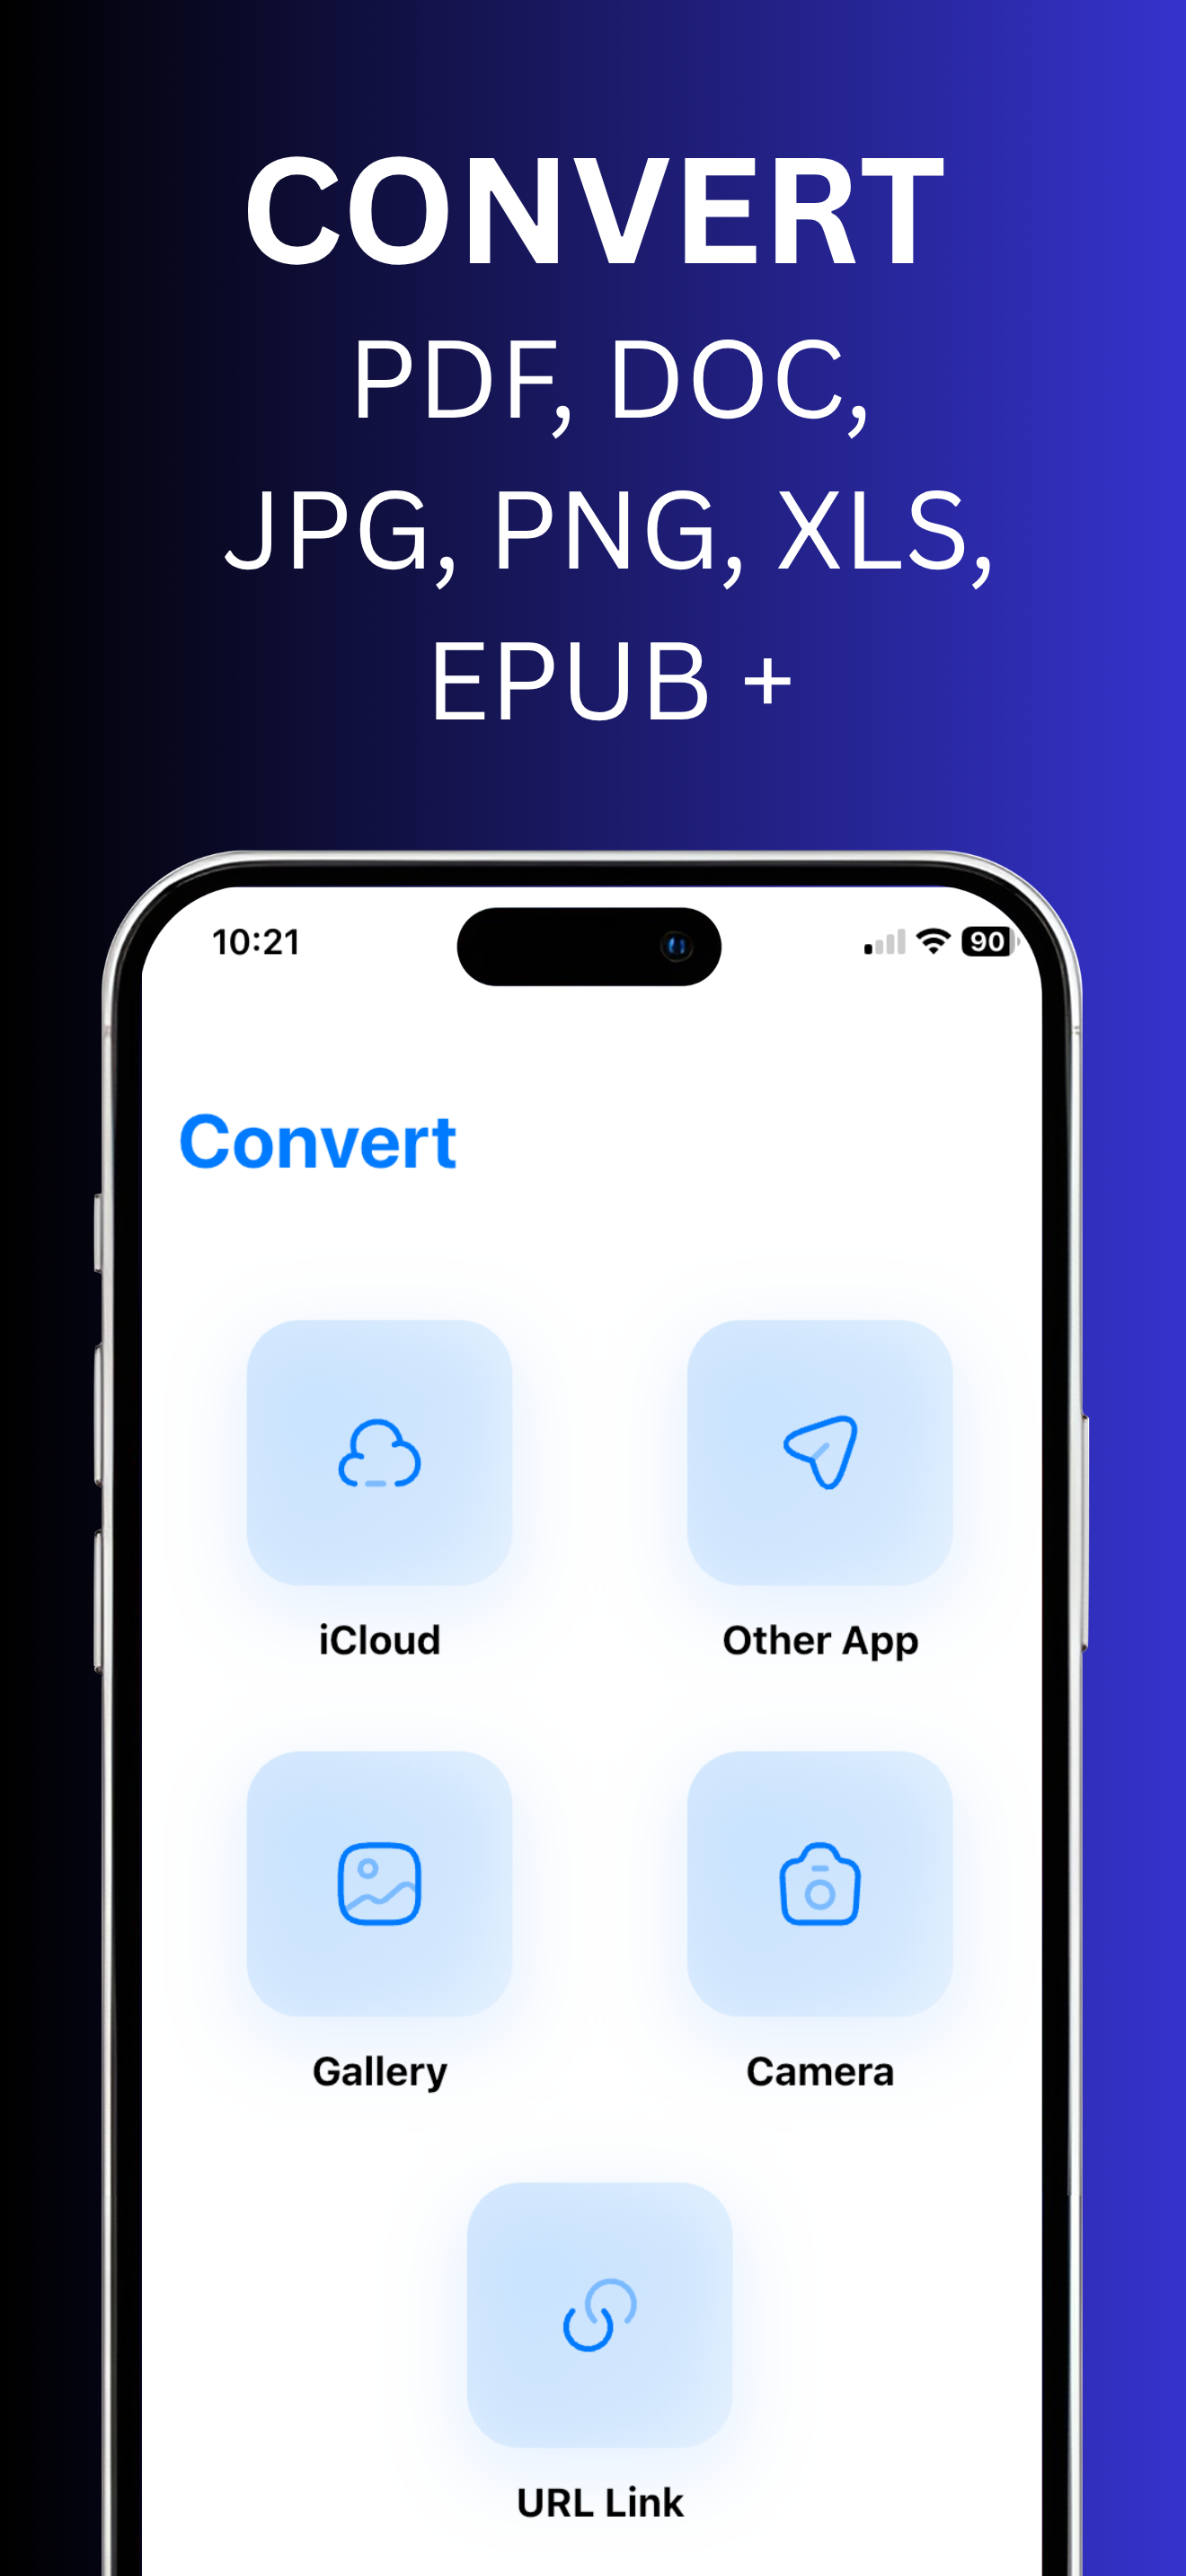
\includegraphics[width=\textwidth]{screenshots/3.png}\\
    \vspace{0.1cm}
    \scriptsize Chọn nguồn
\end{minipage}
\hfill
\begin{minipage}[b]{0.18\textwidth}
    \centering
    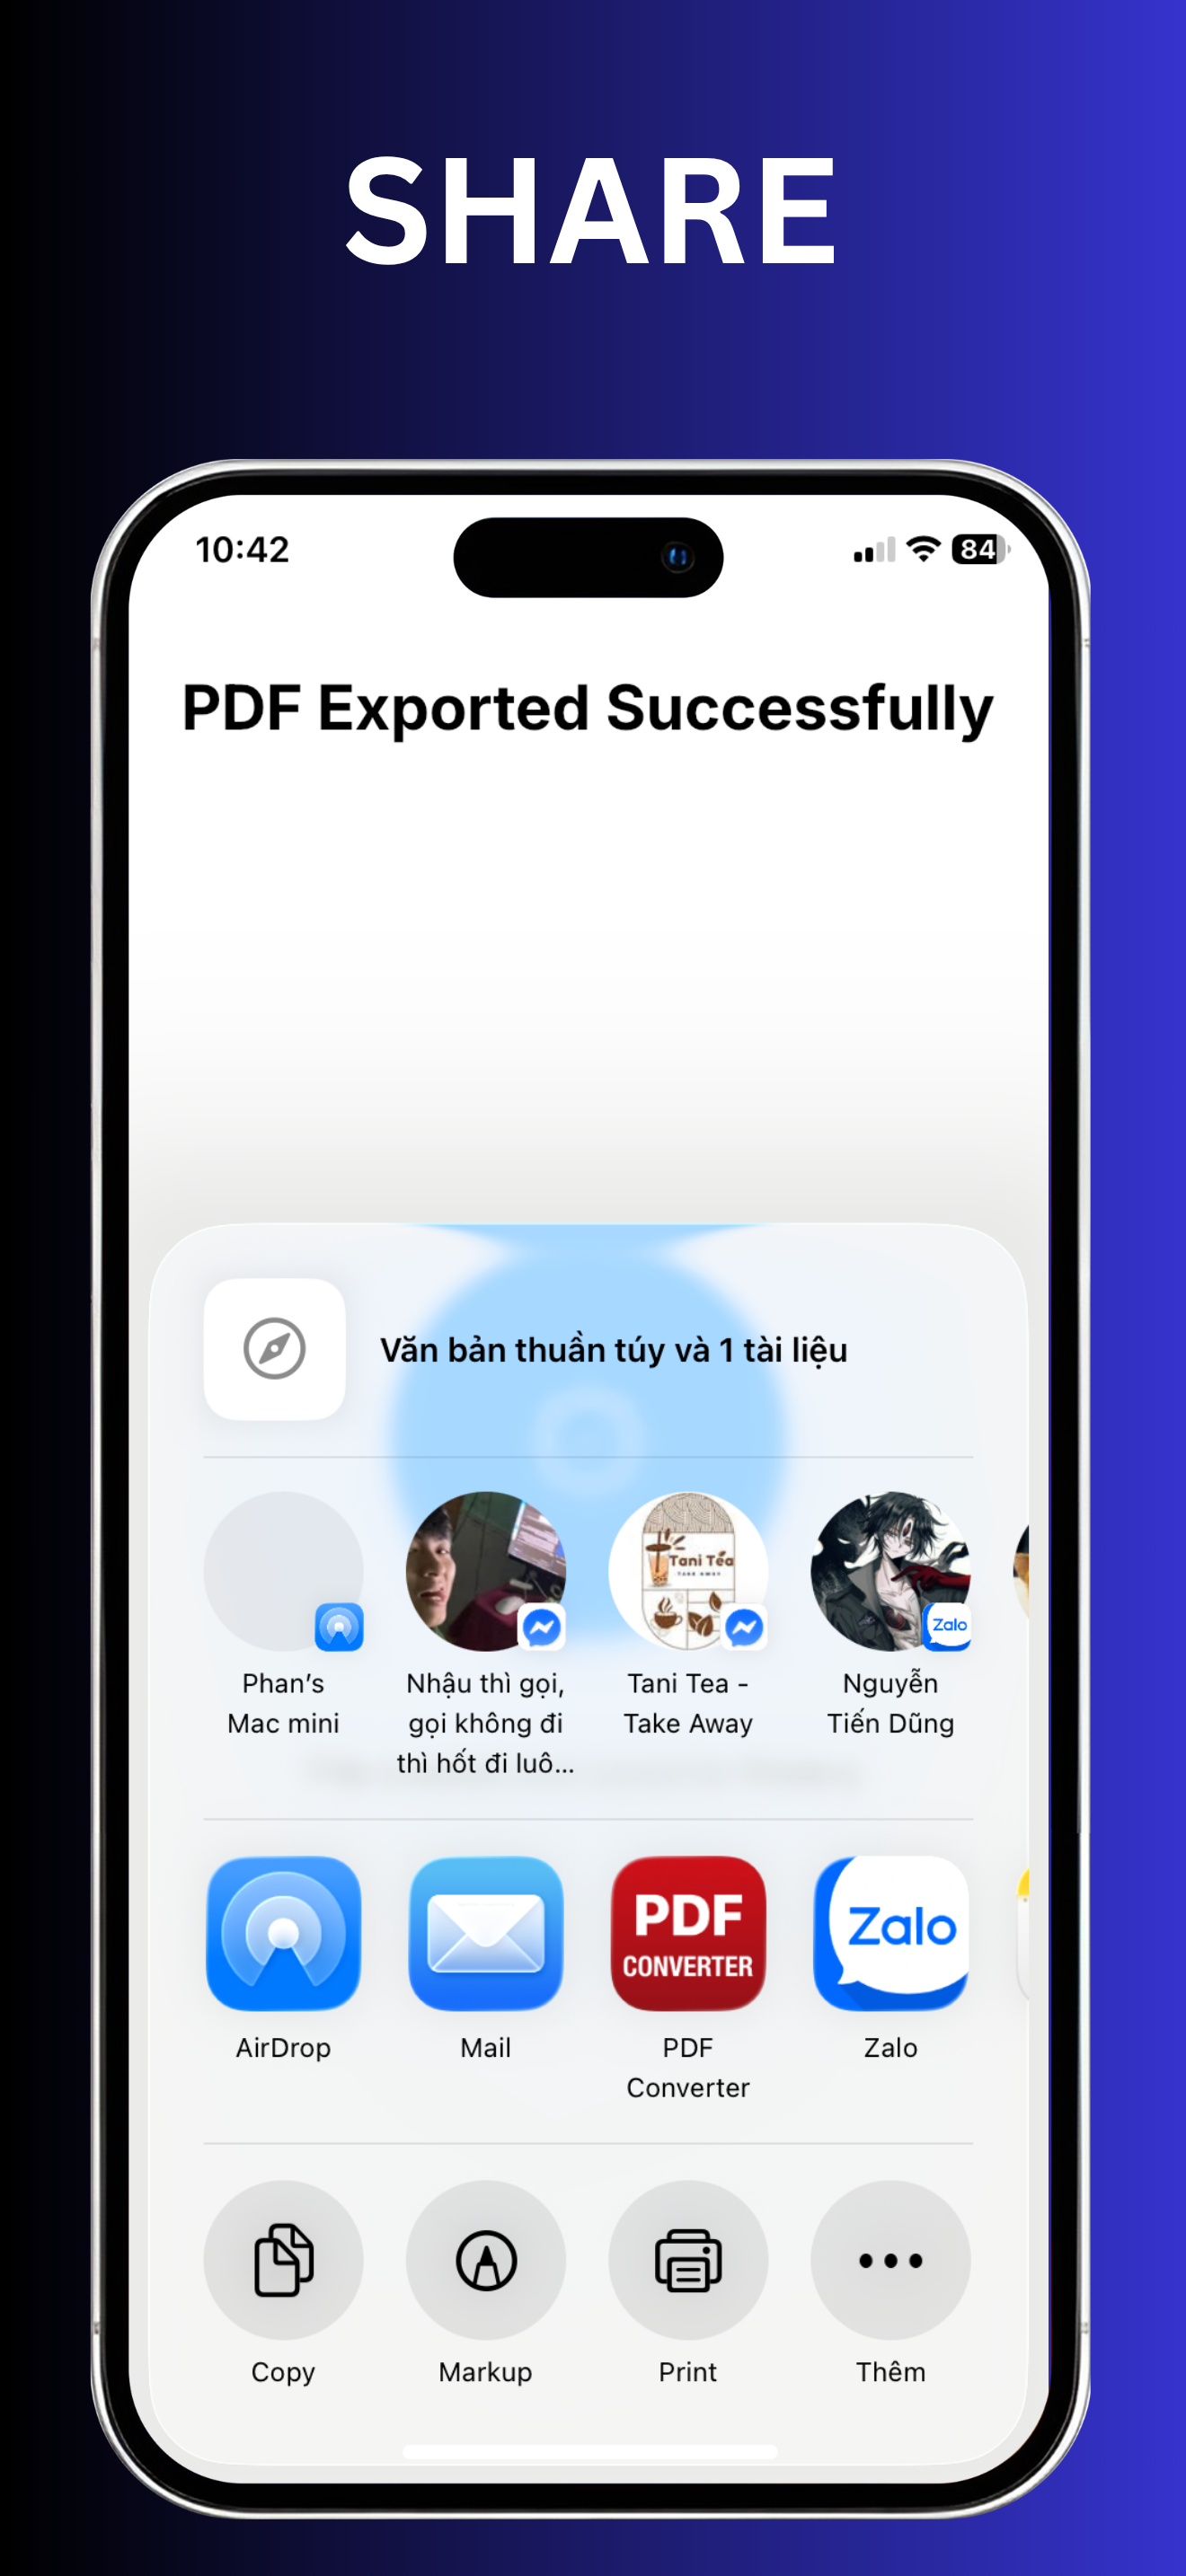
\includegraphics[width=\textwidth]{screenshots/4.png}\\
    \vspace{0.1cm}
    \scriptsize Xuất tệp PDF
\end{minipage}
\hfill
\begin{minipage}[b]{0.18\textwidth}
    \centering
    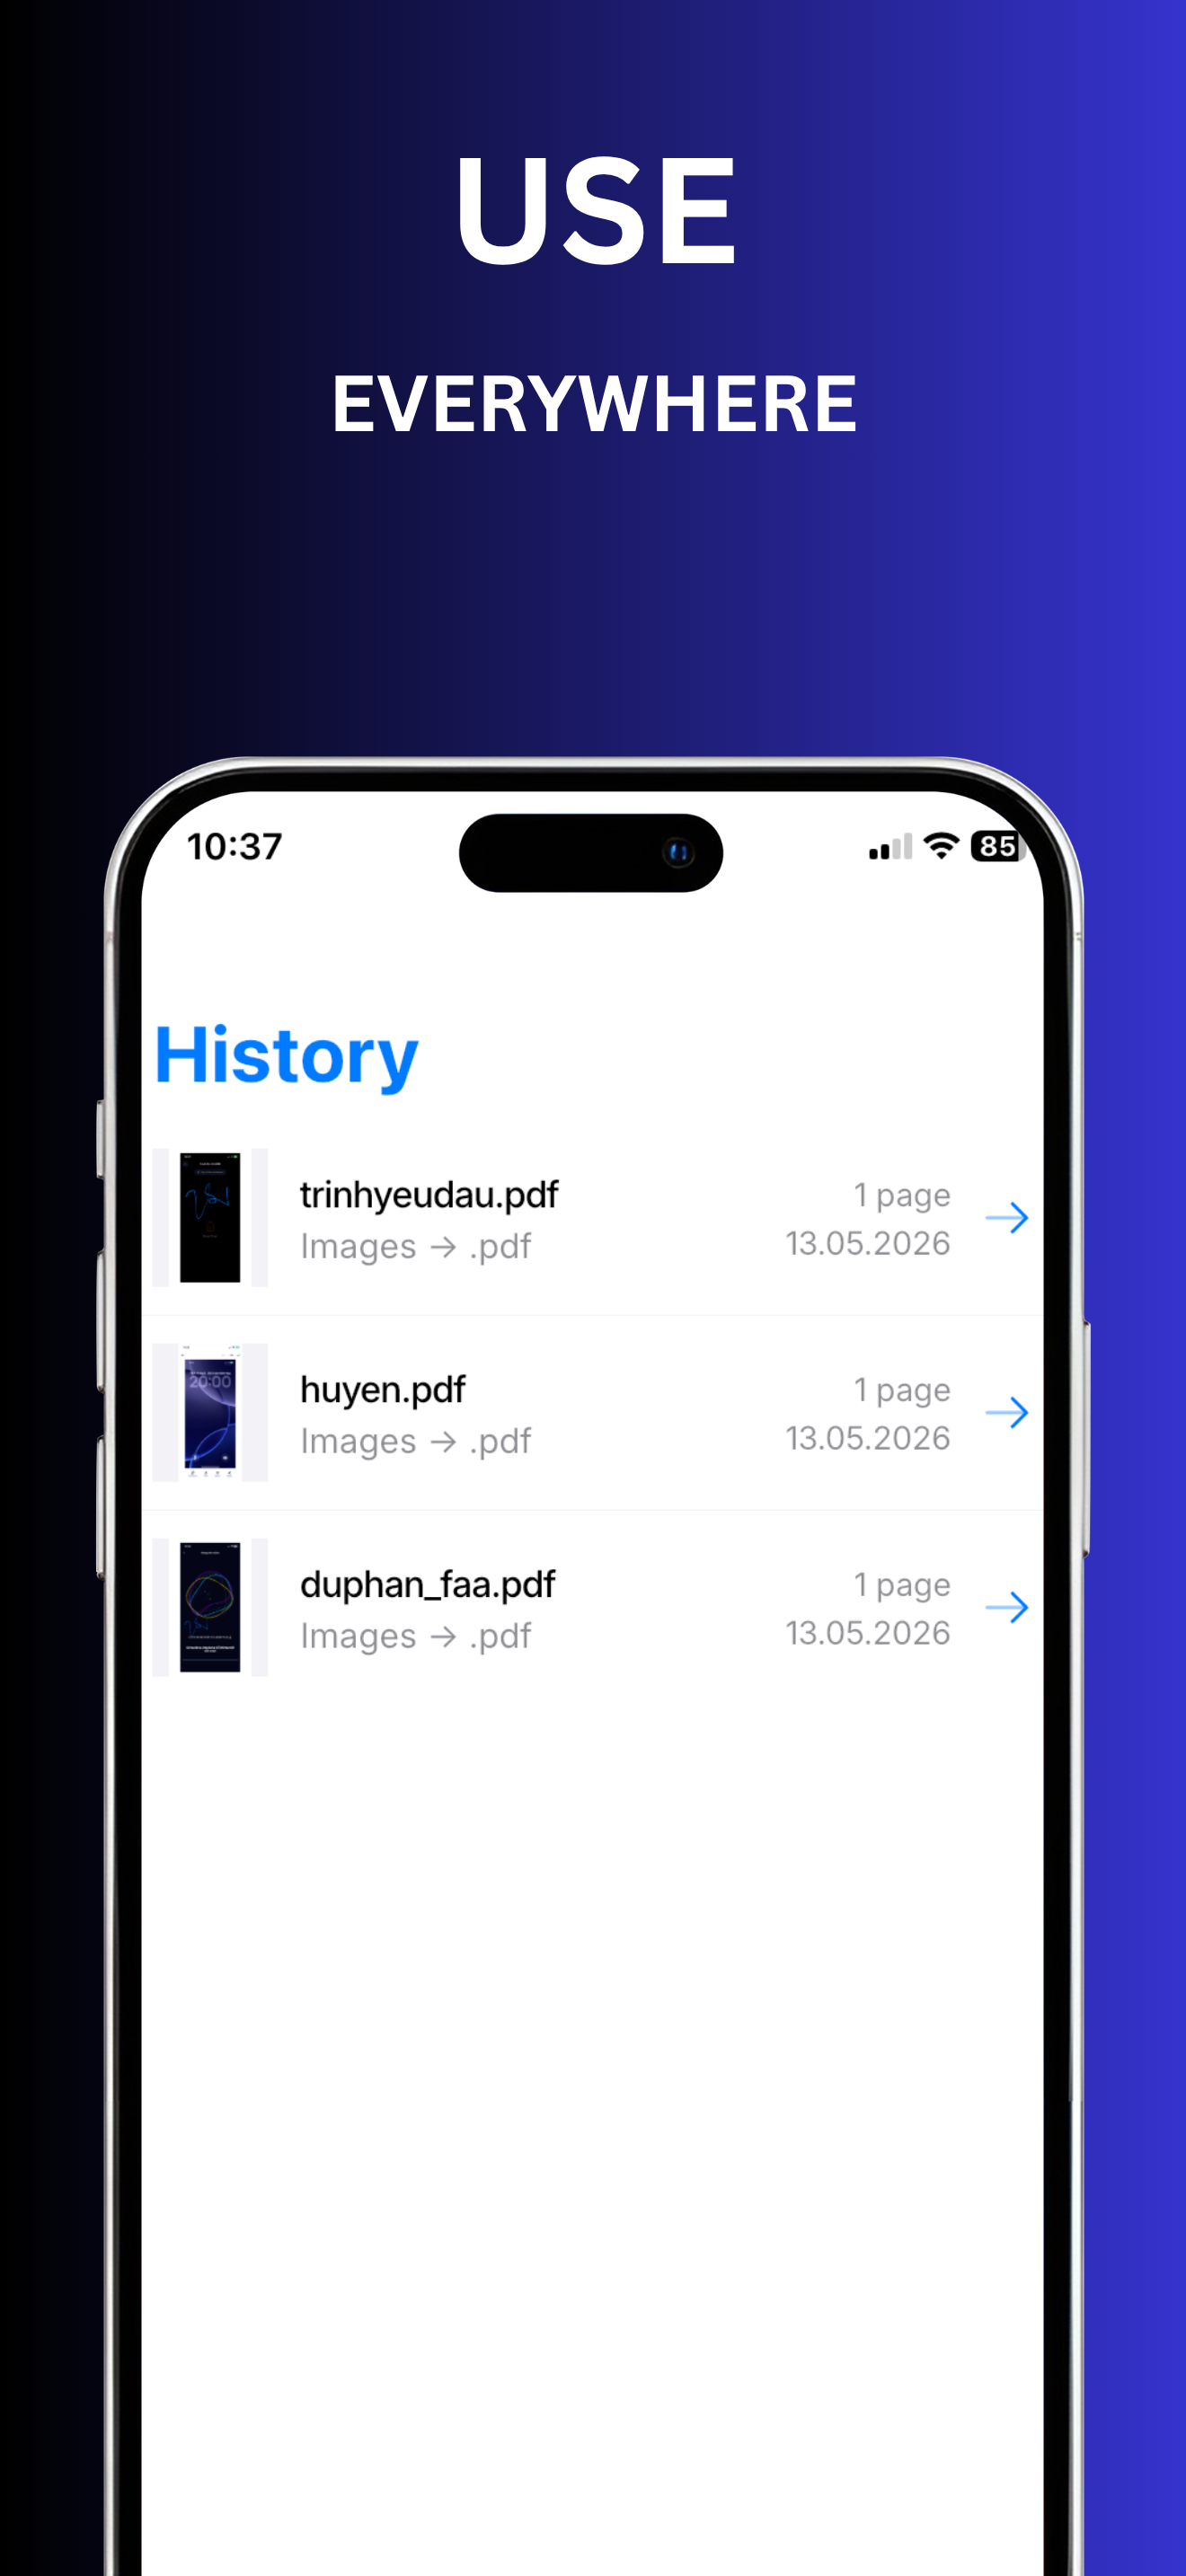
\includegraphics[width=\textwidth]{screenshots/5.png}\\
    \vspace{0.1cm}
    \scriptsize Lịch sử lưu
\end{minipage}
\caption{Giao diện thực tế của ứng dụng PDF Converter \& Scanner trên hệ điều hành iOS}
\label{fig:pdf_converter_screenshots}
\end{figure}

\subsubsection{Dự án Cleaner Guru - Tối ưu hóa doanh thu quảng cáo (Ads Optimization)}
\begin{itemize}
    \item \textbf{Tối ưu hóa AdMob SDK:} Nghiên cứu tích hợp quảng cáo Splash Ads và Interstitial Ads của Google AdMob, đảm bảo phân bổ hợp lý để không làm phiền trải nghiệm dọn dẹp kho ảnh của người dùng.
    \item \textbf{Khắc phục lỗi hiển thị quảng cáo:} Khắc phục triệt để lỗi quảng cáo Splash Ads đã được tải thành công và báo trạng thái sẵn sàng nhưng không thể trình chiếu do xung đột vòng đời Widget và xung đột luồng vẽ UI của Flutter. Tái cấu trúc lại cơ chế gọi callback bất đồng bộ an toàn giúp quảng cáo hiển thị mượt mà.
\end{itemize}

\subsubsection{Dự án Ad-Free Blood Pressure App - Phát hành và tối ưu tăng trưởng}
Đánh dấu mốc quan trọng khi đưa sản phẩm thực tế lên cửa hàng ứng dụng toàn cầu:
\begin{itemize}
    \item \textbf{Deploy thành công lên App Store:} Đổi tên chính thức dự án cá nhân ở giai đoạn 2 thành ứng dụng \textbf{Ad-Free Blood Pressure App} và hoàn tất các thủ tục phát hành thành công trên App Store tại đường dẫn: \url{https://apps.apple.com/us/app/ad-free-blood-pressure-app/id6749716071}.
    \item \textbf{Kết quả tăng trưởng đầu tiên:} Chỉ sau **1 tuần** xuất bản, ứng dụng đã xuất sắc đạt mốc **hơn 100 người dùng hoạt động** (organic users) tự nhiên.
    \item \textbf{Tối ưu hóa liên tục:} Hiện tại đang tiếp tục triển khai tối ưu hóa ad mediation để tối đa hóa doanh thu từ quảng cáo và phát triển thêm các biểu đồ phân tích huyết áp nâng cao.
\end{itemize}

\begin{figure}[htbp]
\centering
\begin{minipage}[b]{0.45\textwidth}
    \centering
    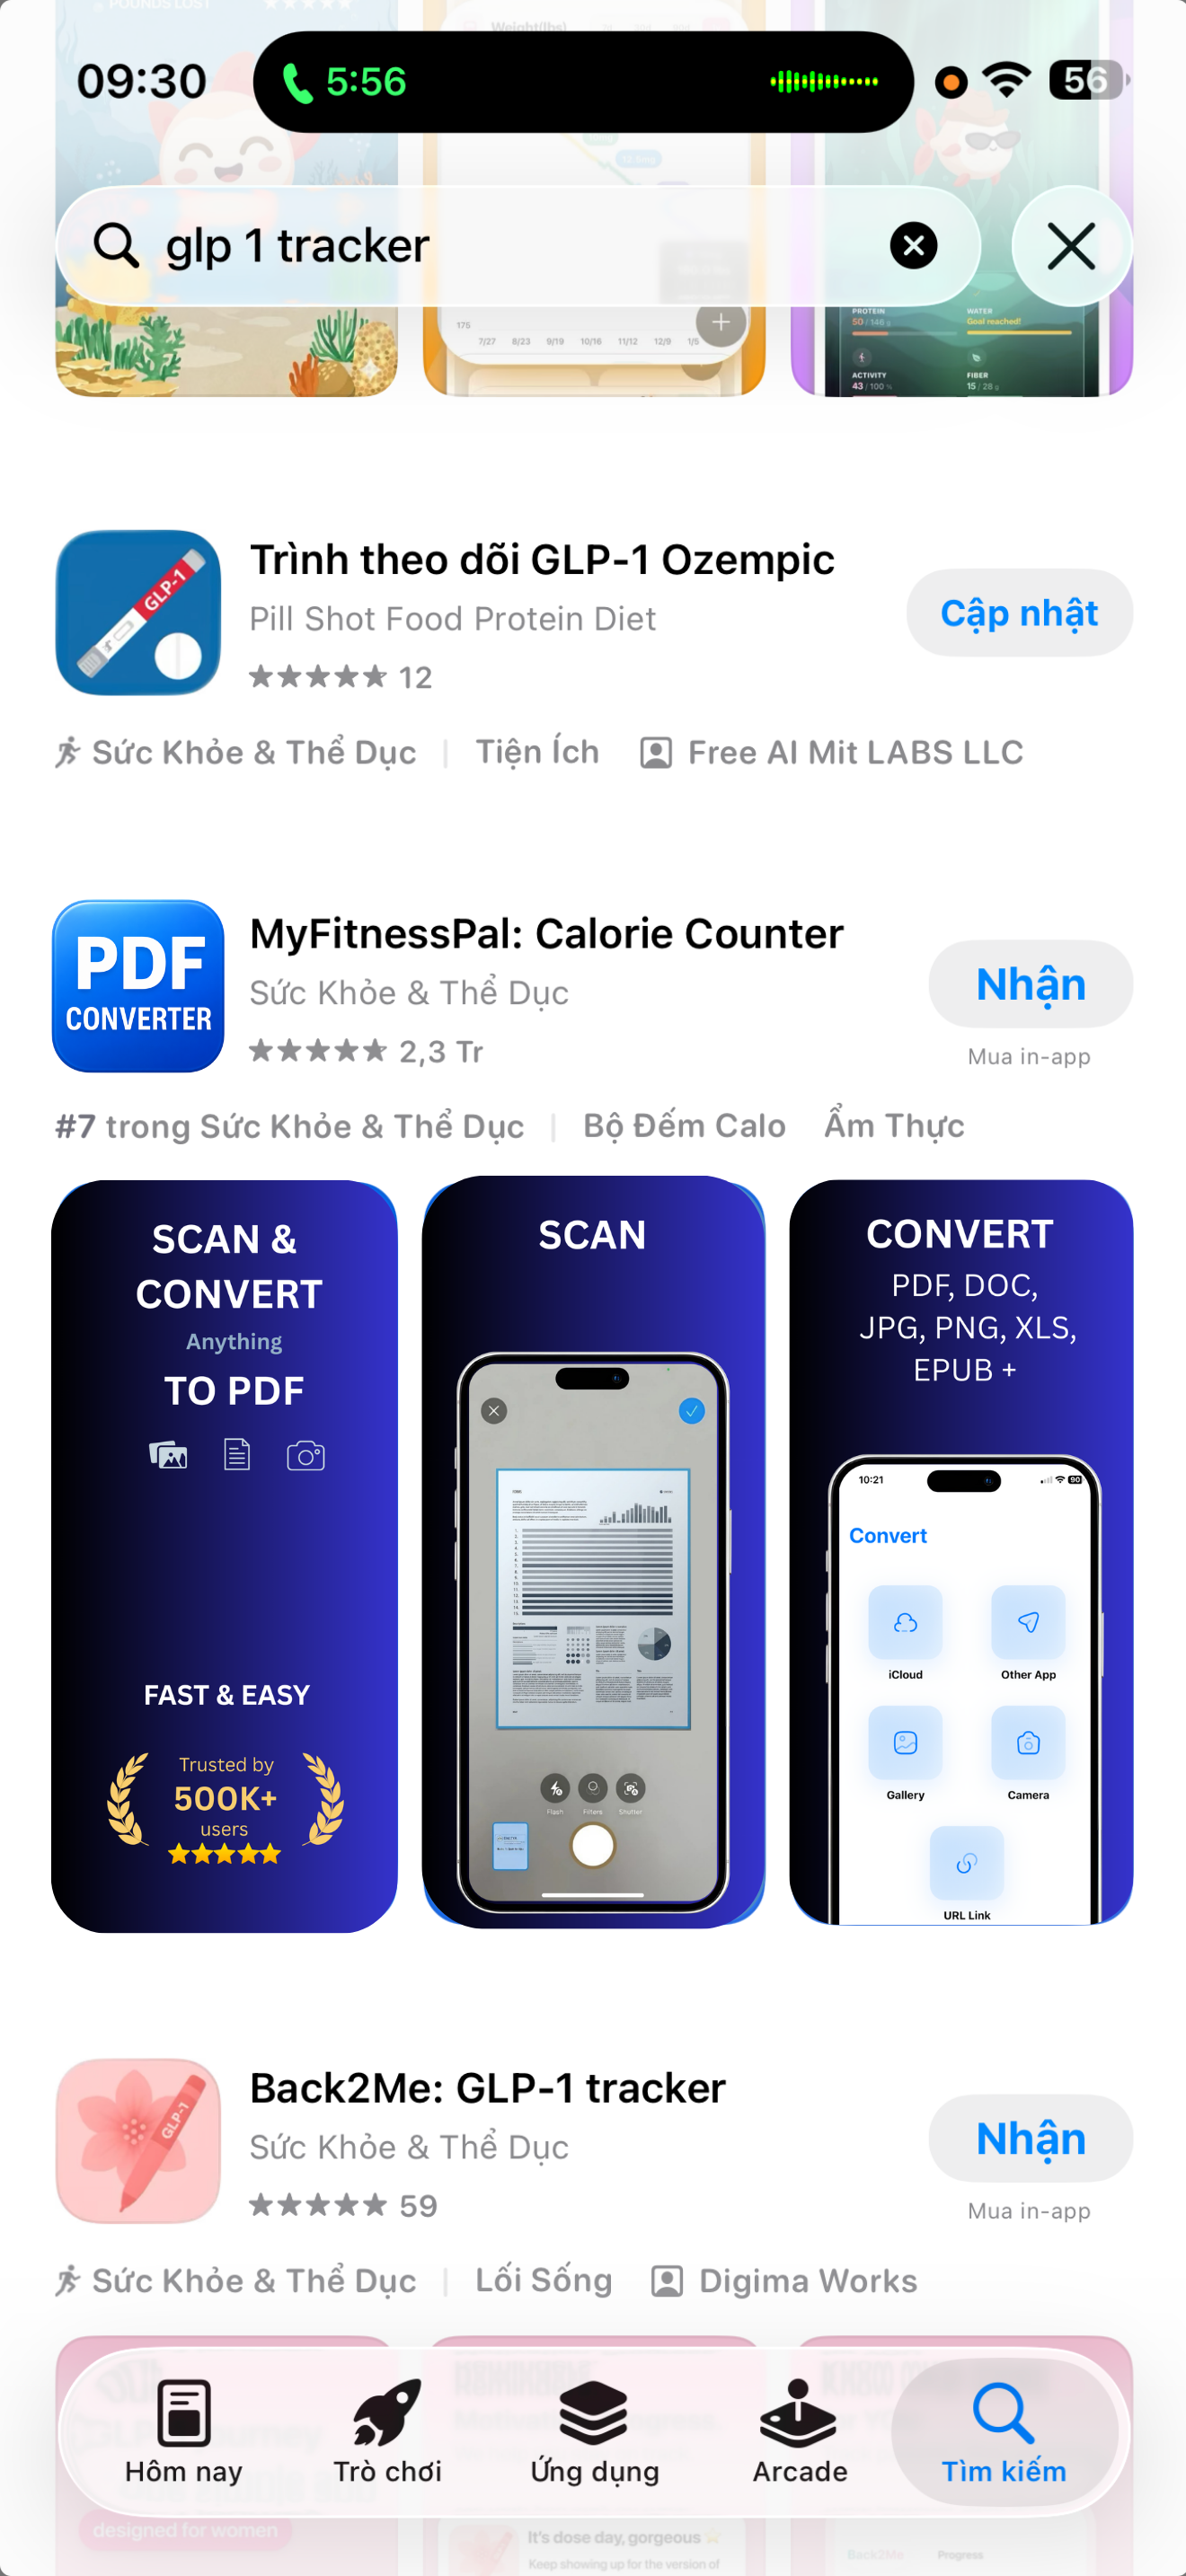
\includegraphics[width=\textwidth]{demo_app_store/1.png}\\
    \vspace{0.1cm}
    \scriptsize Giao diện App Store (Chế độ Sáng)
\end{minipage}
\hfill
\begin{minipage}[b]{0.45\textwidth}
    \centering
    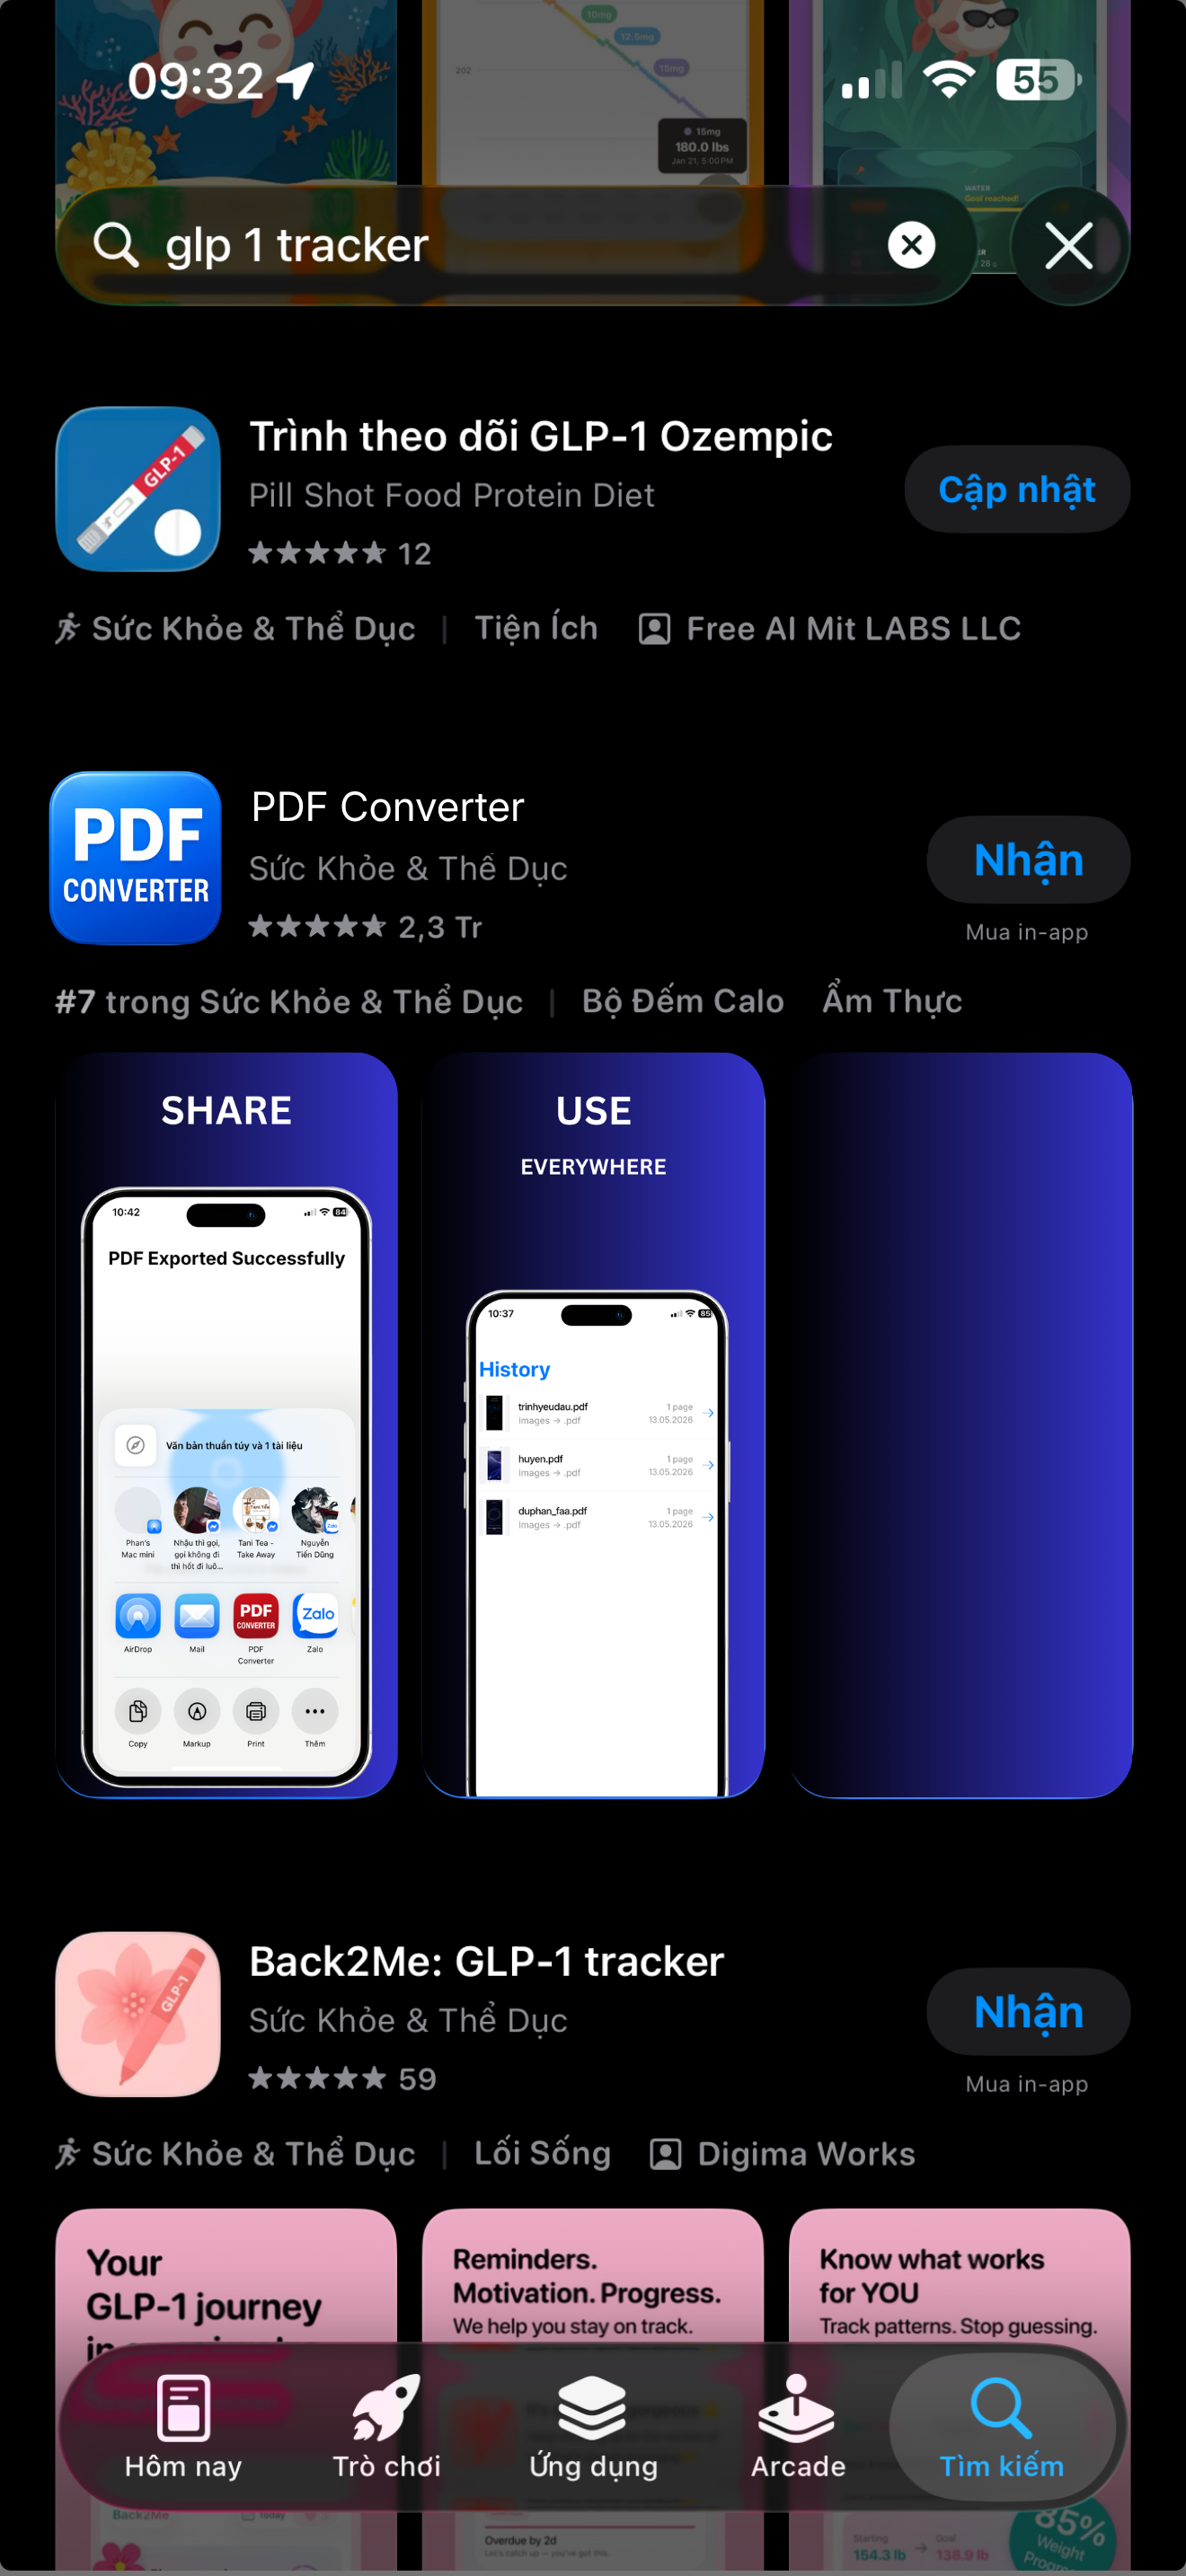
\includegraphics[width=\textwidth]{demo_app_store/2.png}\\
    \vspace{0.1cm}
    \scriptsize Giao diện App Store (Chế độ Tối)
\end{minipage}
\caption{Hình ảnh hiển thị thực tế của ứng dụng trên cửa hàng App Store}
\label{fig:app_store_screenshots}
\end{figure}



\section{TỰ ĐÁNH GIÁ VÀ BÀI HỌC KINH NGHIỆM}

\subsection{Điểm mạnh và Sự trưởng thành}
\begin{itemize}
    \item \textbf{Năng lực chuyên môn:} Đã làm chủ được các kỹ thuật lập trình Mobile nâng cao như xử lý luồng (Isolate), giao tiếp hệ điều hành (Method Channel) và đặc biệt là kỹ thuật xử lý tín hiệu sinh trắc học (PPG) và thị giác máy tính (Computer Vision).
    \item \textbf{Tư duy sản phẩm:} Chuyển đổi từ tư duy "làm cho chạy" sang tư duy "tối ưu cho người dùng". Biết chú trọng vào hiệu suất phần cứng (RAM/CPU) và trải nghiệm người dùng thực tế trên các dòng máy cấu hình thấp.
    \item \textbf{Khả năng thích nghi:} Nhanh chóng nắm bắt các công cụ hỗ trợ hiện đại như Cursor AI kết hợp với quy trình làm việc chuẩn Agile/Scrum, giúp tối ưu hóa 30-40\% thời gian phát triển dự án.
\end{itemize}

\subsection{Hạn chế và Những thách thức cần vượt qua}
\begin{itemize}
    \item \textbf{Kỹ thuật chuyên sâu:} Các thuật toán xử lý ảnh lặp (dHash) hoặc đo nhịp tim (PPG) đôi khi vẫn gặp sai số trong môi trường ánh sáng cực yếu. Đây là mảng kiến thức khó, đòi hỏi nghiên cứu sâu hơn về xử lý tín hiệu số.
    \item \textbf{Kỹ năng trình bày:} Khả năng diễn giải các cấu trúc thuật toán phức tạp thông qua sơ đồ (Diagram) vẫn cần được rèn luyện thêm để tăng tính minh bạch trong trong việc báo cáo kỹ thuật với Mentor.
\end{itemize}

\subsection{Bài học kinh nghiệm quý báu}
Thông qua đợt thực tập kéo dài hơn một năm, em đã rút ra những bài học xương sống:
\begin{itemize}
    \item Tầm quan trọng của việc viết mã nguồn sạch (Clean Code) và tuân thủ kiến trúc chuẩn ngay từ đầu để dễ dàng bảo trì và mở rộng khi quy mô nhóm tăng lên.
    \item Kỹ năng làm việc nhóm không chỉ là code chung, mà là sự thấu hiểu quy trình, trách nhiệm với từng Ticket trên Jira và sự tôn trọng tuyệt đối với Git Flow của tập thể.
\end{itemize}

\section{KẾT QUẢ TỔNG THỂ VÀ ĐỊNH HƯỚNG}

\subsection{Kết quả đạt được}
\begin{itemize}
    \item \textbf{Hoàn thành các mốc tiến độ:} Đã trực tiếp tham gia phát triển và hỗ trợ hoàn thiện 5 ứng dụng di động đa lĩnh vực bao gồm: \textit{Blood Sugar, Ad-Free Blood Pressure App, Cleaner Guru, Push Up, và PDF Converter \& Scanner}. Trong đó, ứng dụng tự phát triển độc lập \textbf{Ad-Free Blood Pressure App} đã chính thức được phát hành xuất sắc thành công lên App Store toàn cầu, nhanh chóng đạt mốc hơn 100 người dùng hoạt động chỉ sau 1 tuần.
    \item \textbf{Xác nhận năng lực:} Đã được Mentor và Ban lãnh đạo công ty ghi nhận khả năng xử lý tốt các module phức tạp (quét ảnh, nén PDF đa luồng, xử lý ảnh dHash cục bộ, đếm chống đẩy AI, tối ưu hóa Google AdMob SDK) và đủ năng lực để đảm đương các vị trí lập trình viên Flutter chuyên nghiệp.
\end{itemize}

\subsection{Định hướng phát triển trong tương lai}
\begin{itemize}
    \item \textbf{Ngắn hạn:} Tập trung tối ưu hóa hệ thống quảng cáo (ad mediation), sửa lỗi và kiểm thử toàn diện ứng dụng \textit{PDF Converter \& Scanner} để chuẩn bị phát hành chính thức, đồng thời duy trì và cập nhật các tính năng đo huyết áp nâng cao cho \textit{Ad-Free Blood Pressure App}.
    \item \textbf{Dài hạn:} Phấn đấu trở thành một Chuyên gia phát triển ứng dụng di động (Senior Mobile Developer) tại \textbf{FAA Việt Nam}, tập trung nghiên cứu sâu hơn về việc tích hợp trí tuệ nhân tạo (AI/ML) trực tiếp vào thiết bị di động để nâng cao hiệu suất và bảo mật thông tin sức khỏe cho người dùng.
\end{itemize}

\newpage
\section*{PHỤ LỤC: HÌNH ẢNH MINH HỌA GIAO DIỆN ỨNG DỤNG}
\addcontentsline{toc}{section}{PHỤ LỤC: HÌNH ẢNH MINH HỌA GIAO DIỆN ỨNG DỤNG}
Dưới đây là toàn bộ hình ảnh giao diện thực tế ghi nhận kết quả phát triển các ứng dụng di động trong suốt giai đoạn thực tập tính đến ngày 20/05/2026:

\subsection*{Phần 1: Dự án Cleaner Guru (Giai đoạn 2)}
Ứng dụng dọn dẹp ảnh trùng lặp thông minh, giải phóng dung lượng bộ nhớ thiết bị iOS:

\subsubsection*{1.1. Màn hình Onboarding}
\begin{figure}[htbp]
    \centering
    \begin{minipage}{0.45\textwidth}
        \centering
        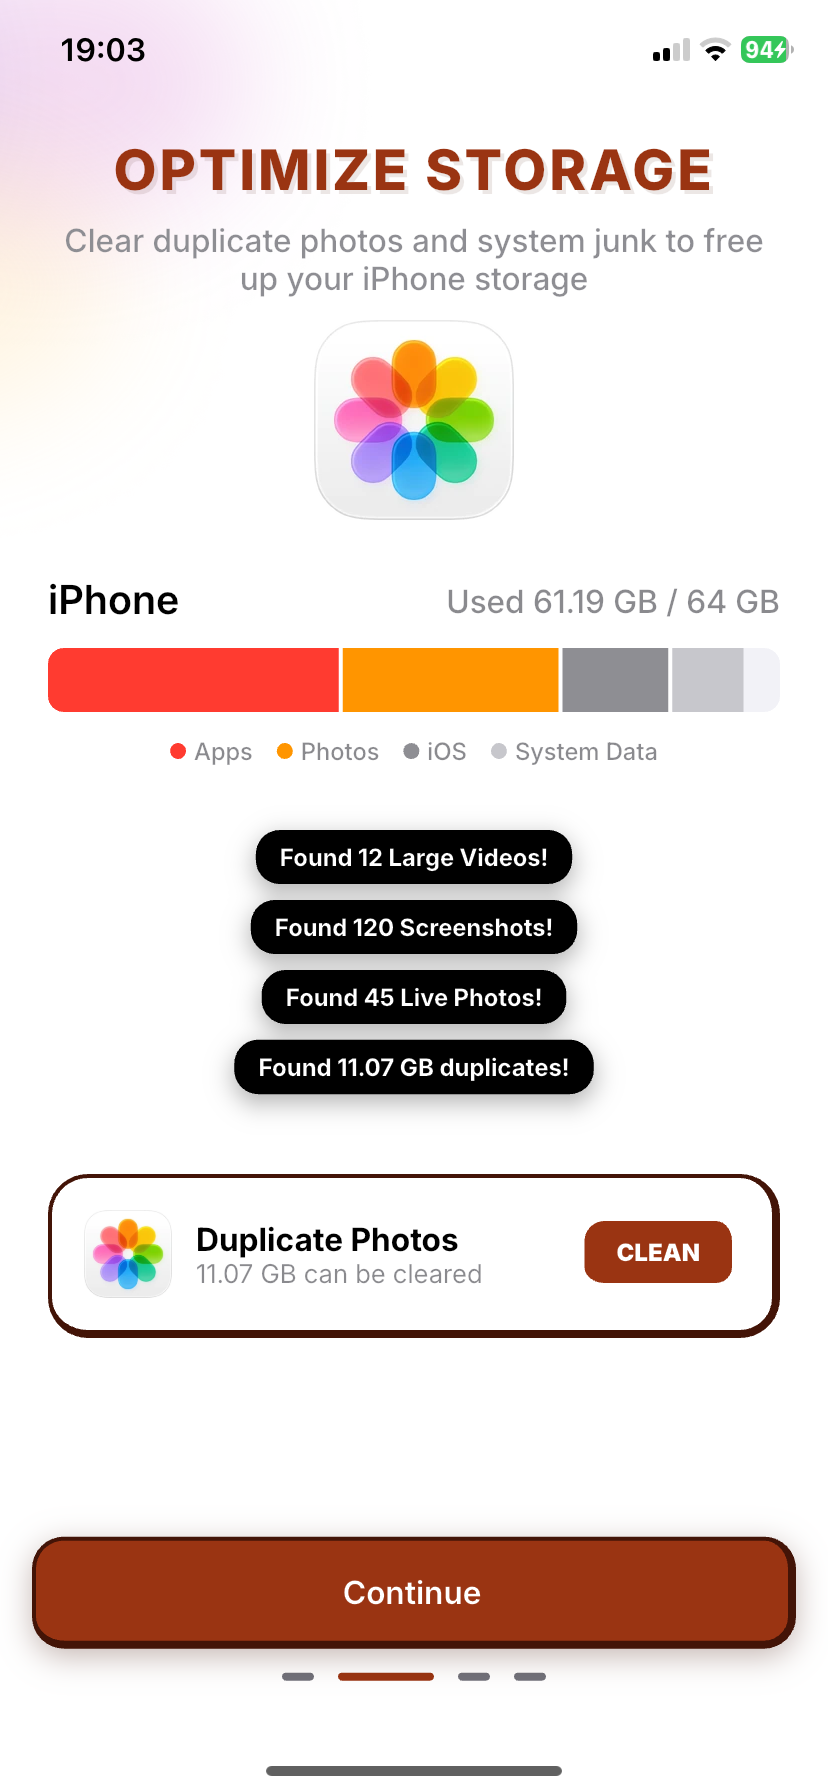
\includegraphics[height=9.5cm]{cleanerguru/IMG_6851.PNG}
        \caption{Onboarding: Giới thiệu tính năng phân tích bộ nhớ lưu trữ.}
        \label{fig:cleaner_onb_storage}
    \end{minipage}
    \hfill
    \begin{minipage}{0.45\textwidth}
        \centering
        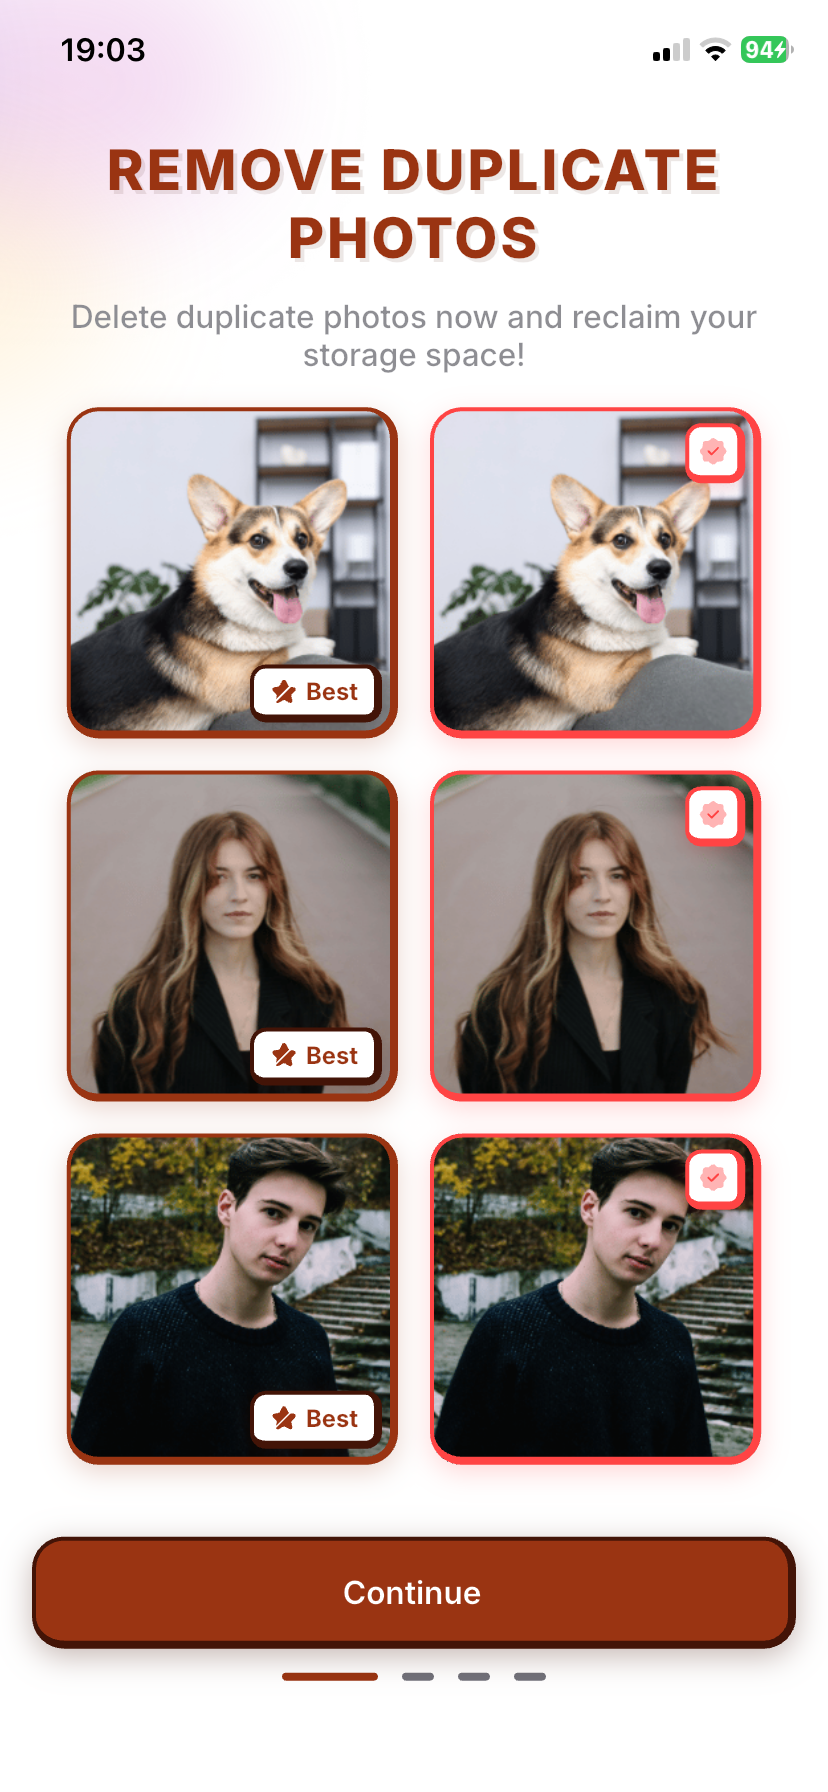
\includegraphics[height=9.5cm]{cleanerguru/IMG_6850.PNG}
        \caption{Onboarding: Giới thiệu tính năng gom nhóm ảnh tương đồng.}
        \label{fig:cleaner_onb_similar}
    \end{minipage}
\end{figure}

\begin{figure}[htbp]
    \centering
    \begin{minipage}{0.45\textwidth}
        \centering
        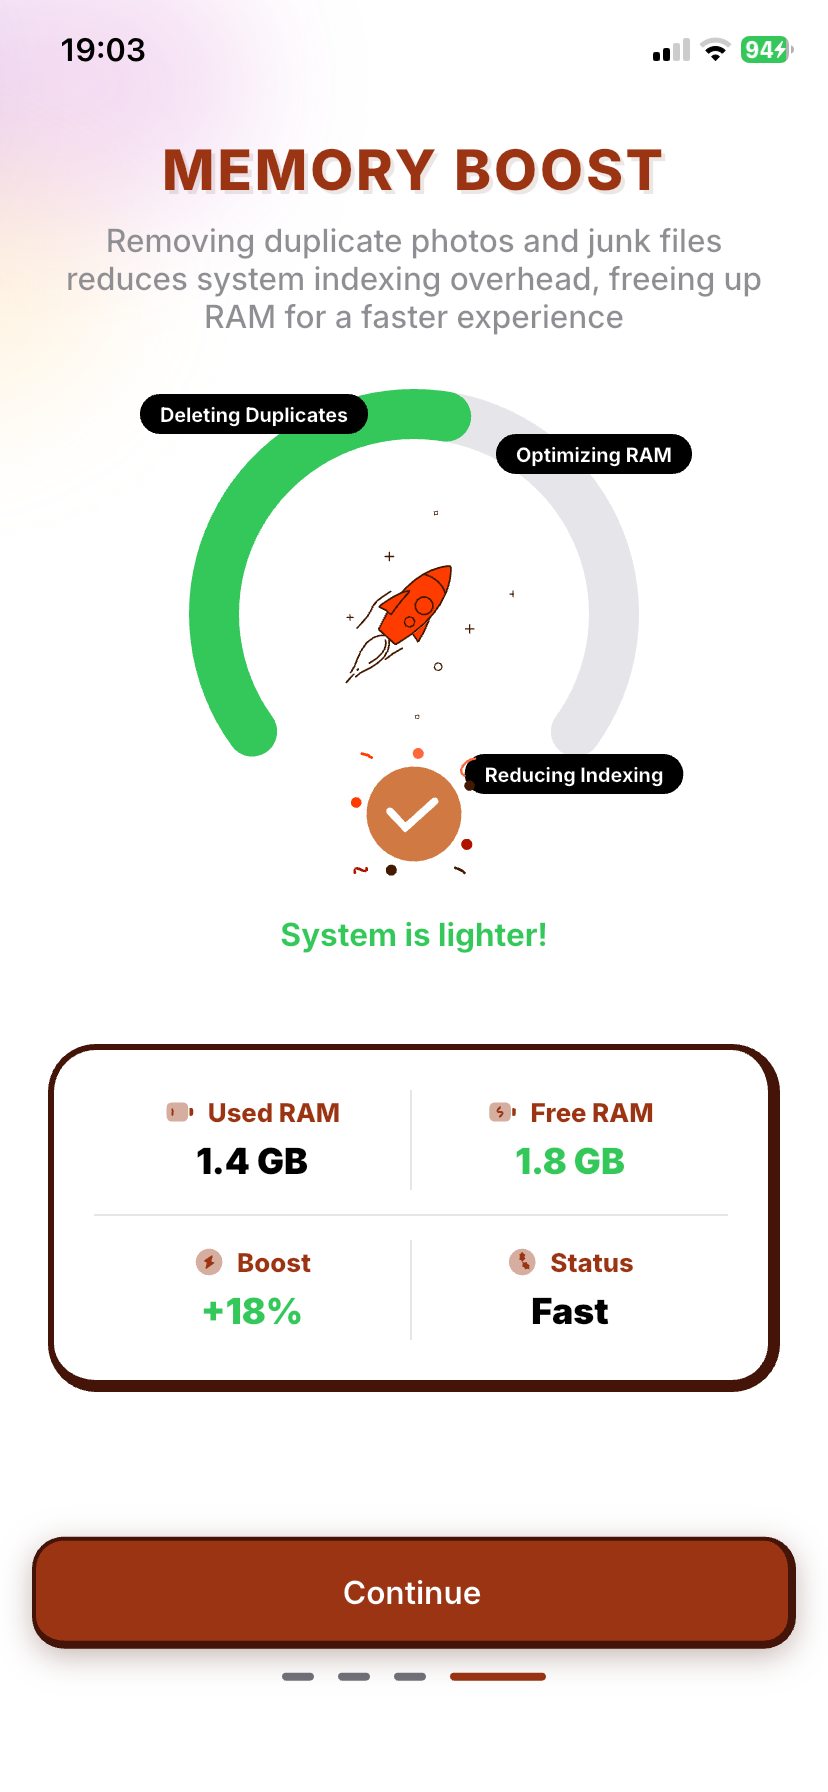
\includegraphics[height=9.5cm]{cleanerguru/IMG_6854.PNG}
        \caption{Onboarding: Giới thiệu tính năng Memory Boost (giải phóng RAM).}
        \label{fig:cleaner_onb_ram}
    \end{minipage}
    \hfill
    \begin{minipage}{0.45\textwidth}
        \centering
        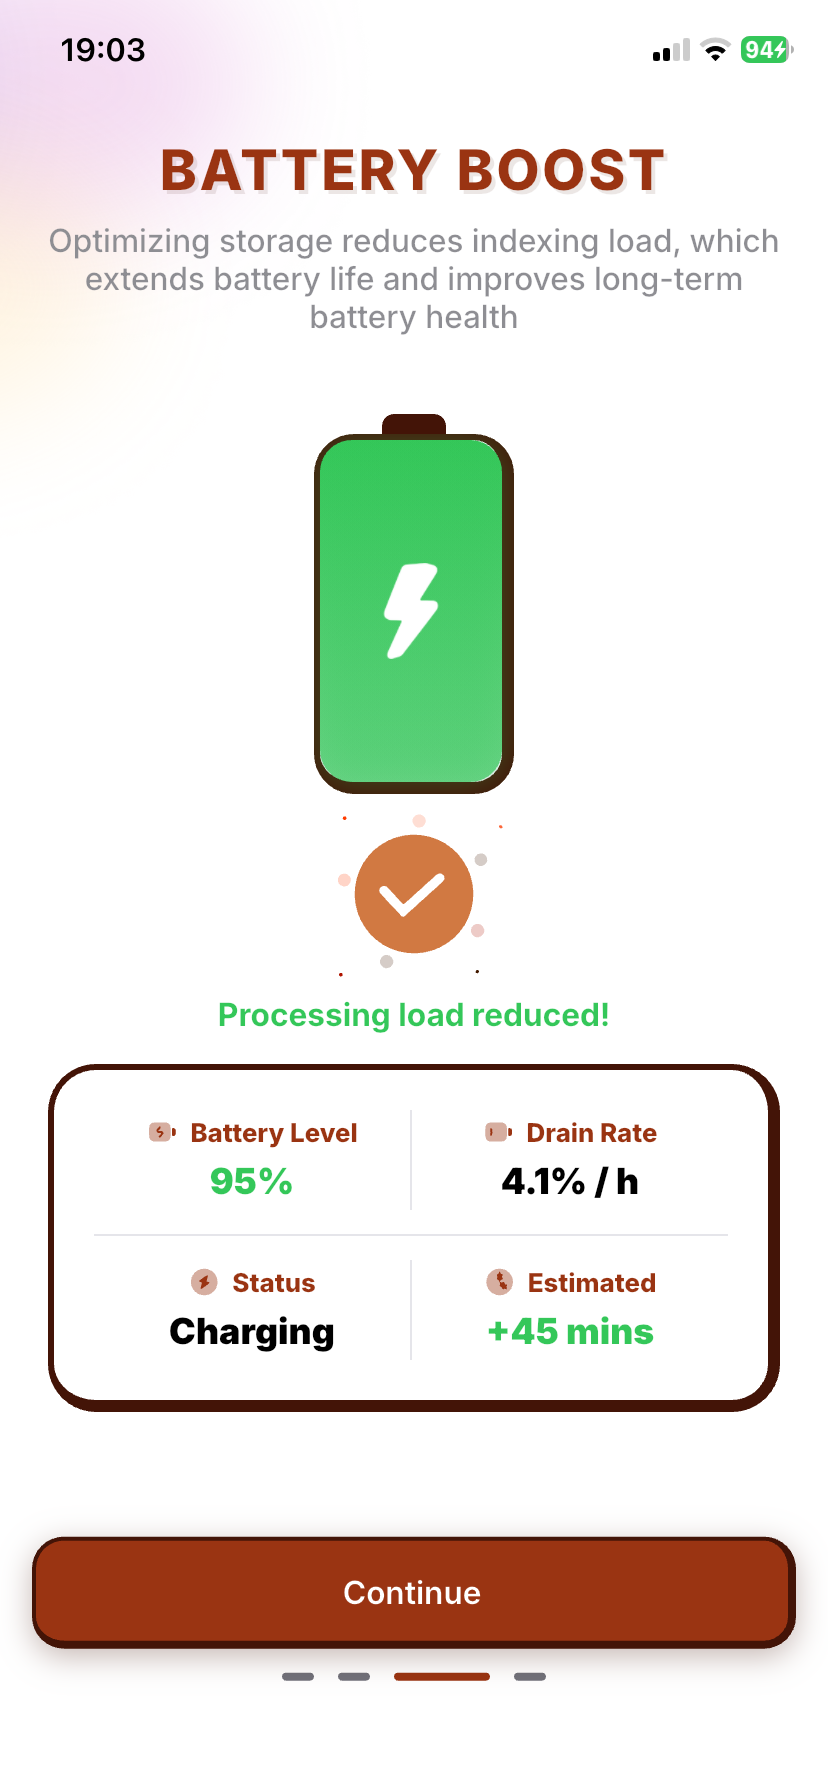
\includegraphics[height=9.5cm]{cleanerguru/IMG_6853.PNG}
        \caption{Onboarding: Giới thiệu tính năng Battery Boost (tối ưu pin).}
        \label{fig:cleaner_onb_battery}
    \end{minipage}
\end{figure}

\newpage
\subsubsection*{1.2. Màn hình Tính năng Chính}
\begin{figure}[htbp]
    \centering
    \begin{minipage}{0.45\textwidth}
        \centering
        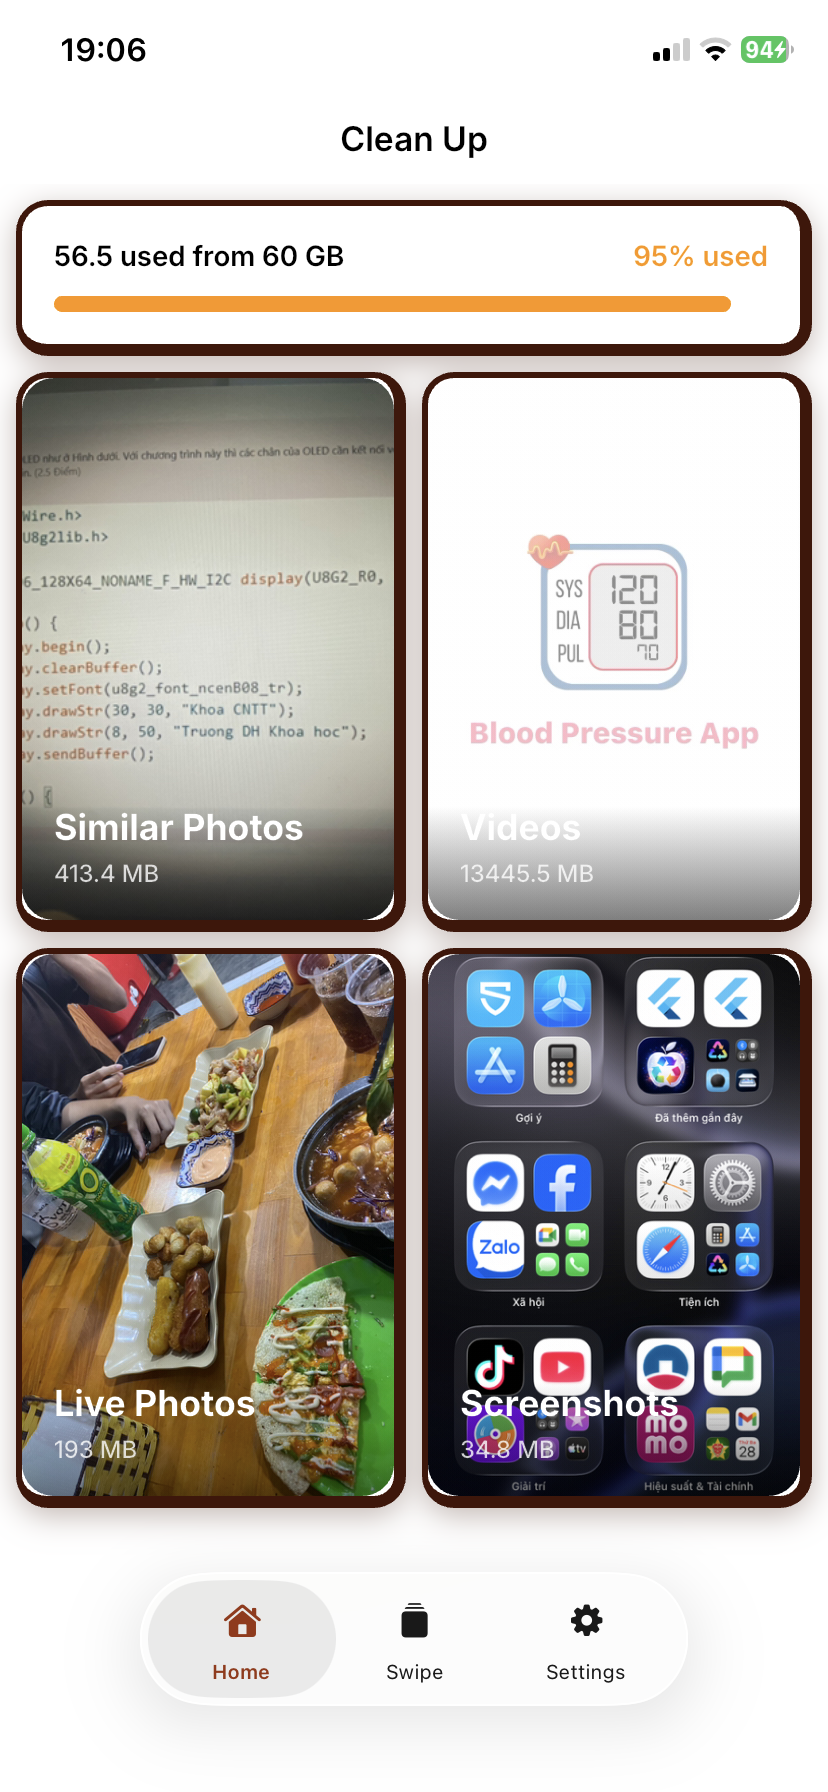
\includegraphics[height=9.5cm]{cleanerguru/IMG_6863.PNG}
        \caption{Màn hình chính Clean Up: phân loại ảnh giống nhau, video, live photo và screenshots theo dung lượng.}
        \label{fig:cleaner_home}
    \end{minipage}
    \hfill
    \begin{minipage}{0.45\textwidth}
        \centering
        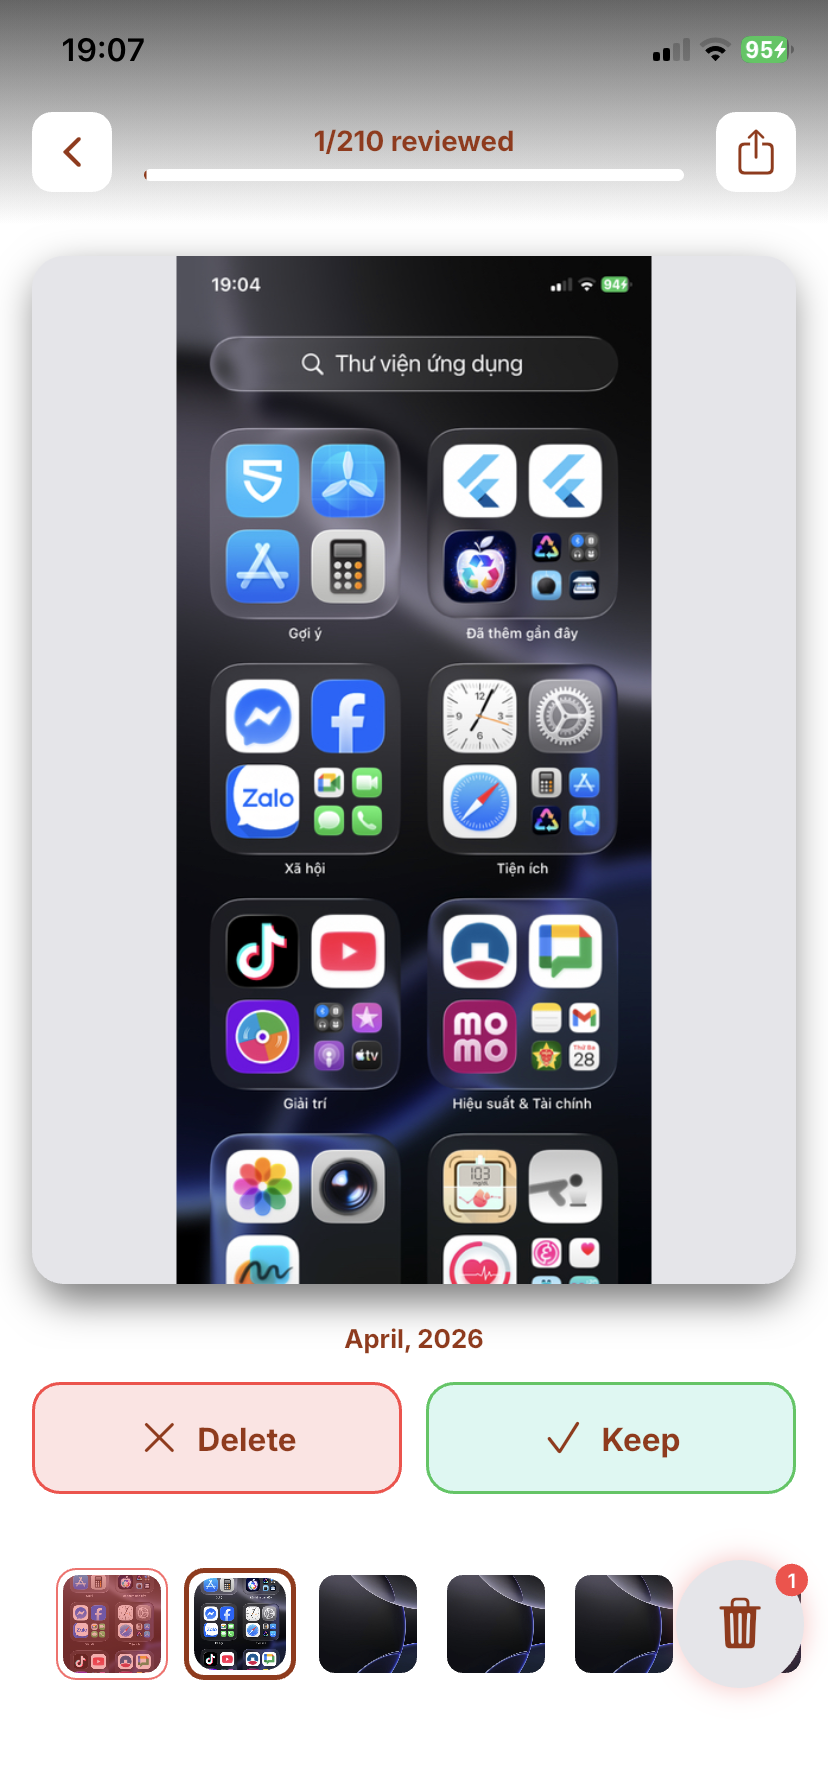
\includegraphics[height=9.5cm]{cleanerguru/IMG_6868.PNG}
        \caption{Giao diện Swipe Photos: đánh giá từng ảnh và chọn giữ lại hoặc xóa (Keep/Delete).}
        \label{fig:cleaner_review}
    \end{minipage}
\end{figure}

\begin{figure}[htbp]
    \centering
    \begin{minipage}{0.45\textwidth}
        \centering
        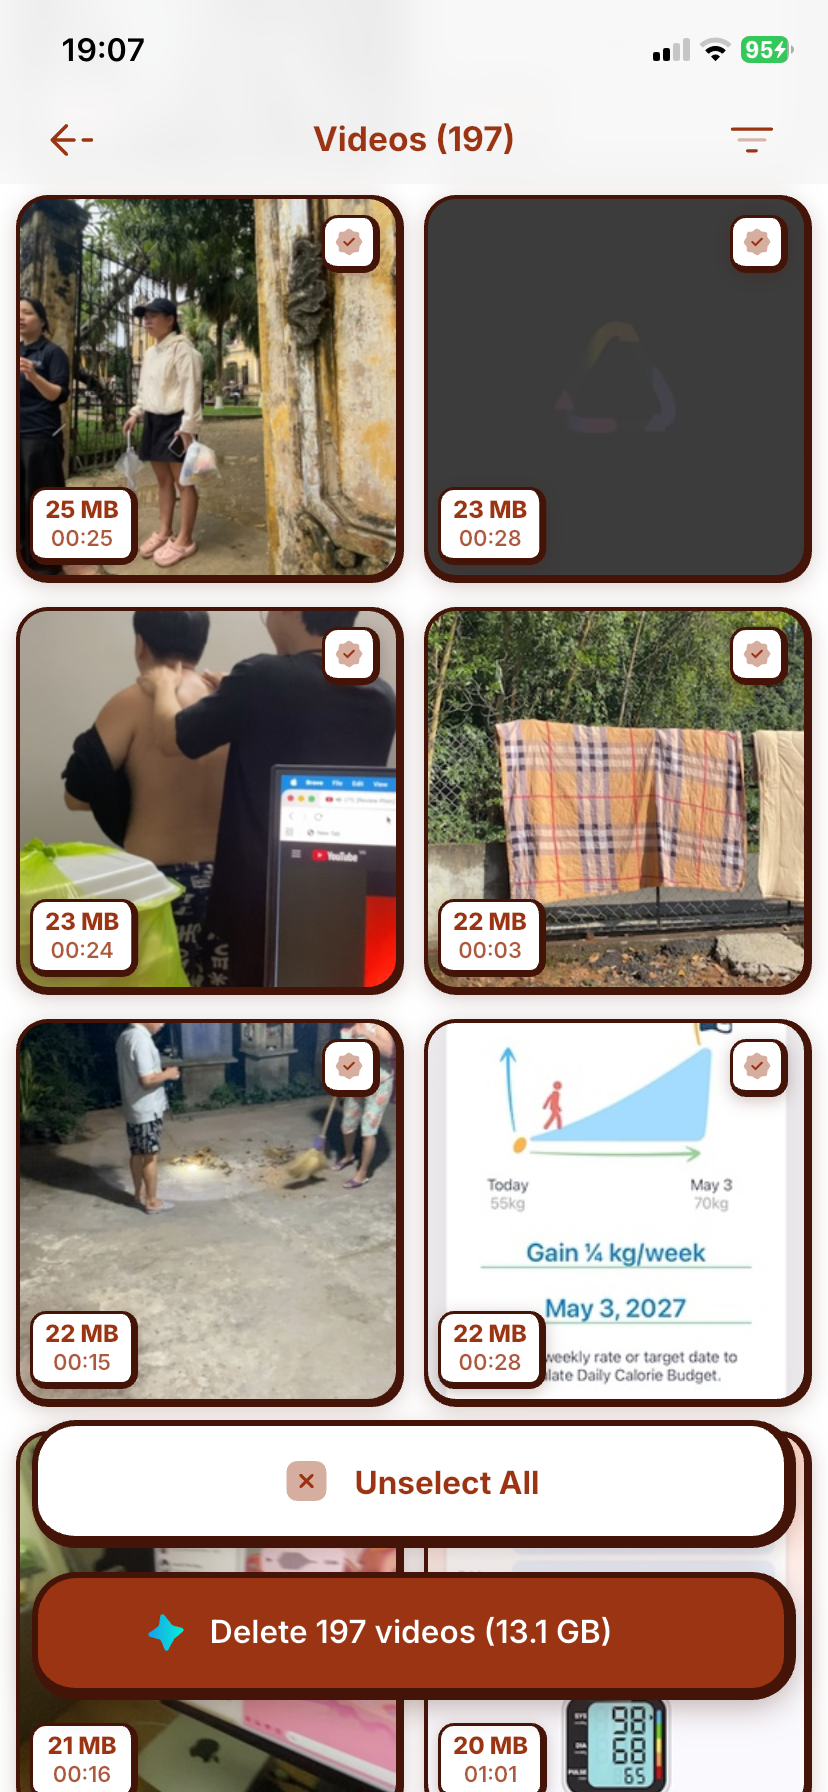
\includegraphics[height=9.5cm]{cleanerguru/IMG_6865.PNG}
        \caption{Màn hình dọn dẹp video dung lượng lớn (197 videos -- 13.1 GB).}
        \label{fig:cleaner_videos}
    \end{minipage}
    \hfill
    \begin{minipage}{0.45\textwidth}
        \centering
        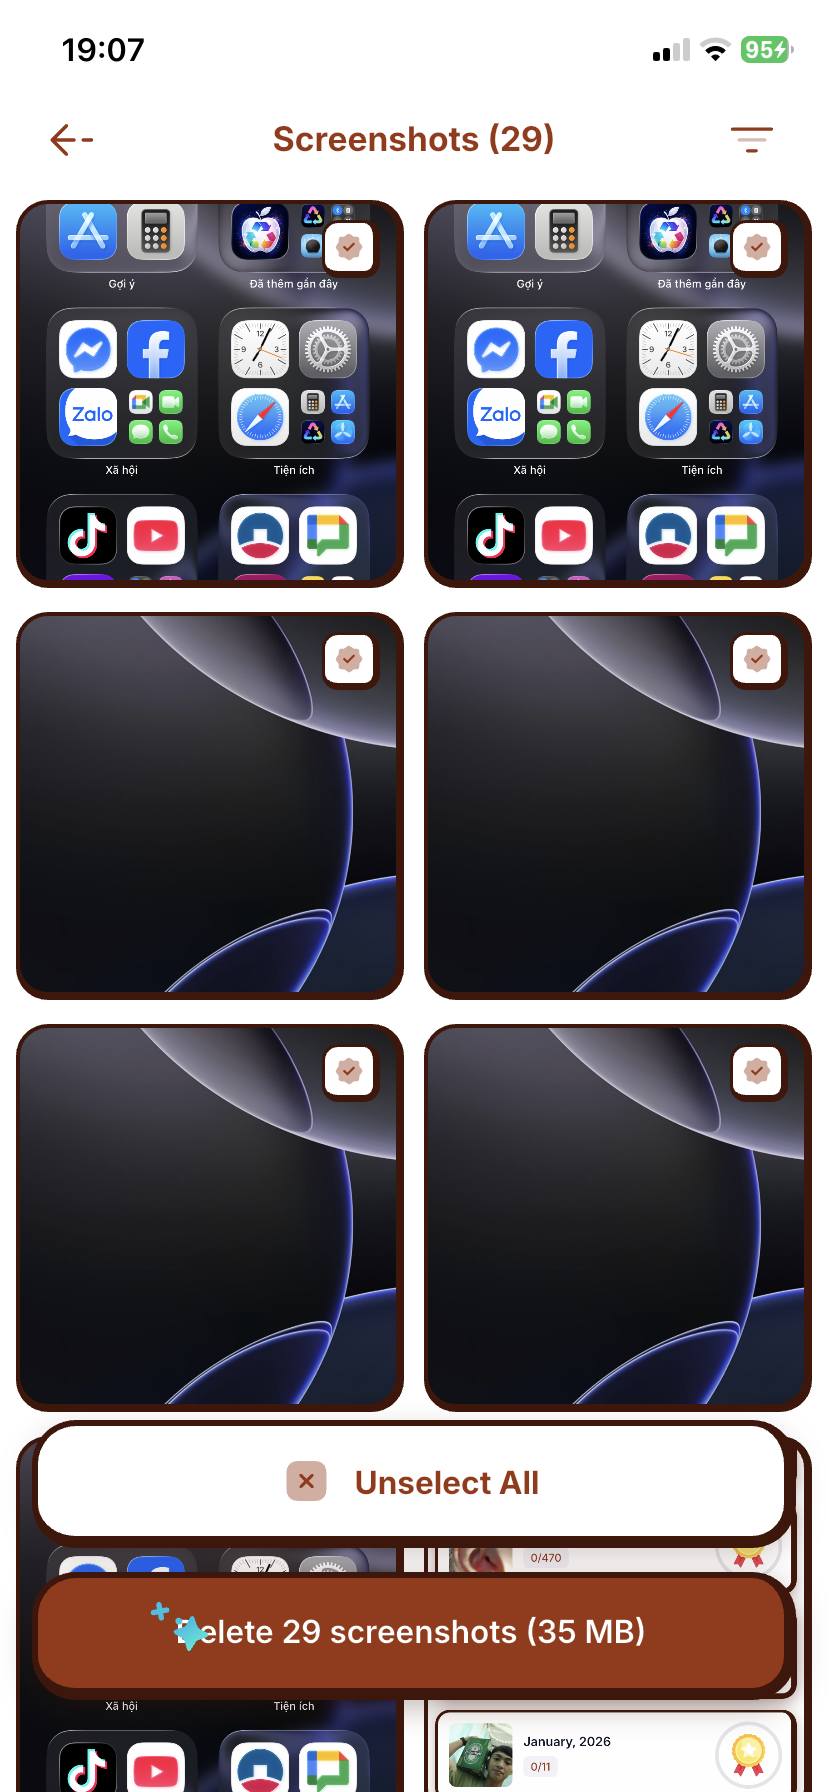
\includegraphics[height=9.5cm]{cleanerguru/IMG_6866.PNG}
        \caption{Màn hình xóa hàng loạt ảnh chụp màn hình trùng lặp (29 screenshots -- 35 MB).}
        \label{fig:cleaner_screenshots}
    \end{minipage}
\end{figure}

\newpage
\subsection*{Phần 2: Dự án Push Up (Giai đoạn 2)}
Ứng dụng hỗ trợ theo dõi sức khỏe và tự động đếm số lần hít đất sử dụng cảm biến tiệm cận:

\begin{figure}[htbp]
    \centering
    \begin{minipage}{0.45\textwidth}
        \centering
        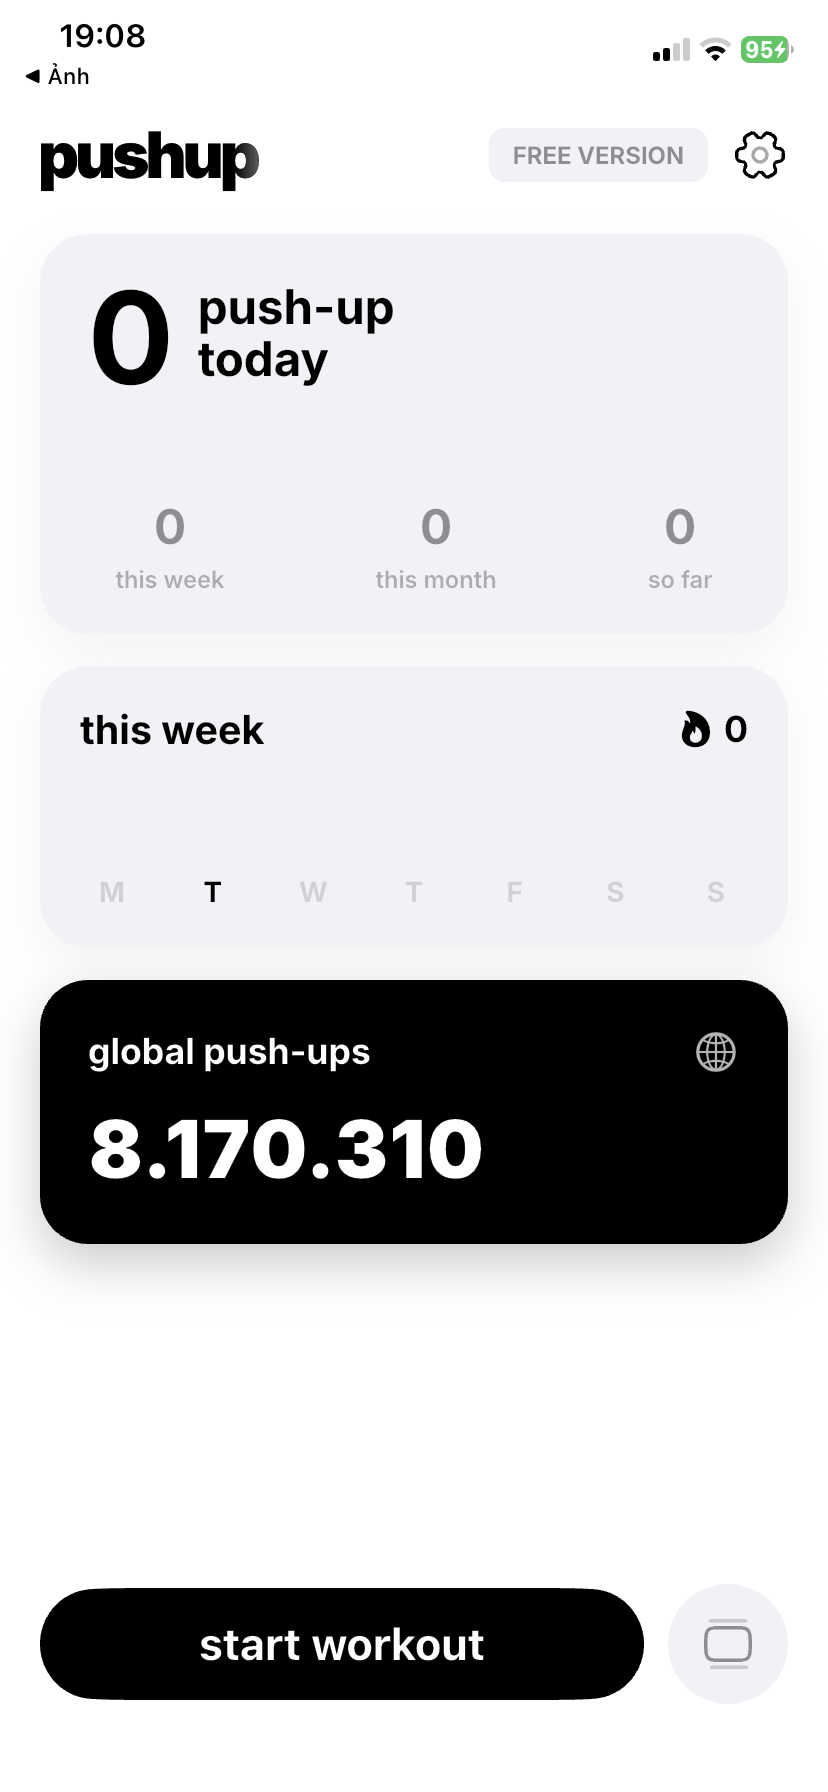
\includegraphics[height=9.5cm]{push_up/IMG_6870.PNG}
        \caption{Màn hình chính thống kê tập luyện (Dashboard).}
        \label{fig:pushup_dash}
    \end{minipage}
    \hfill
    \begin{minipage}{0.45\textwidth}
        \centering
        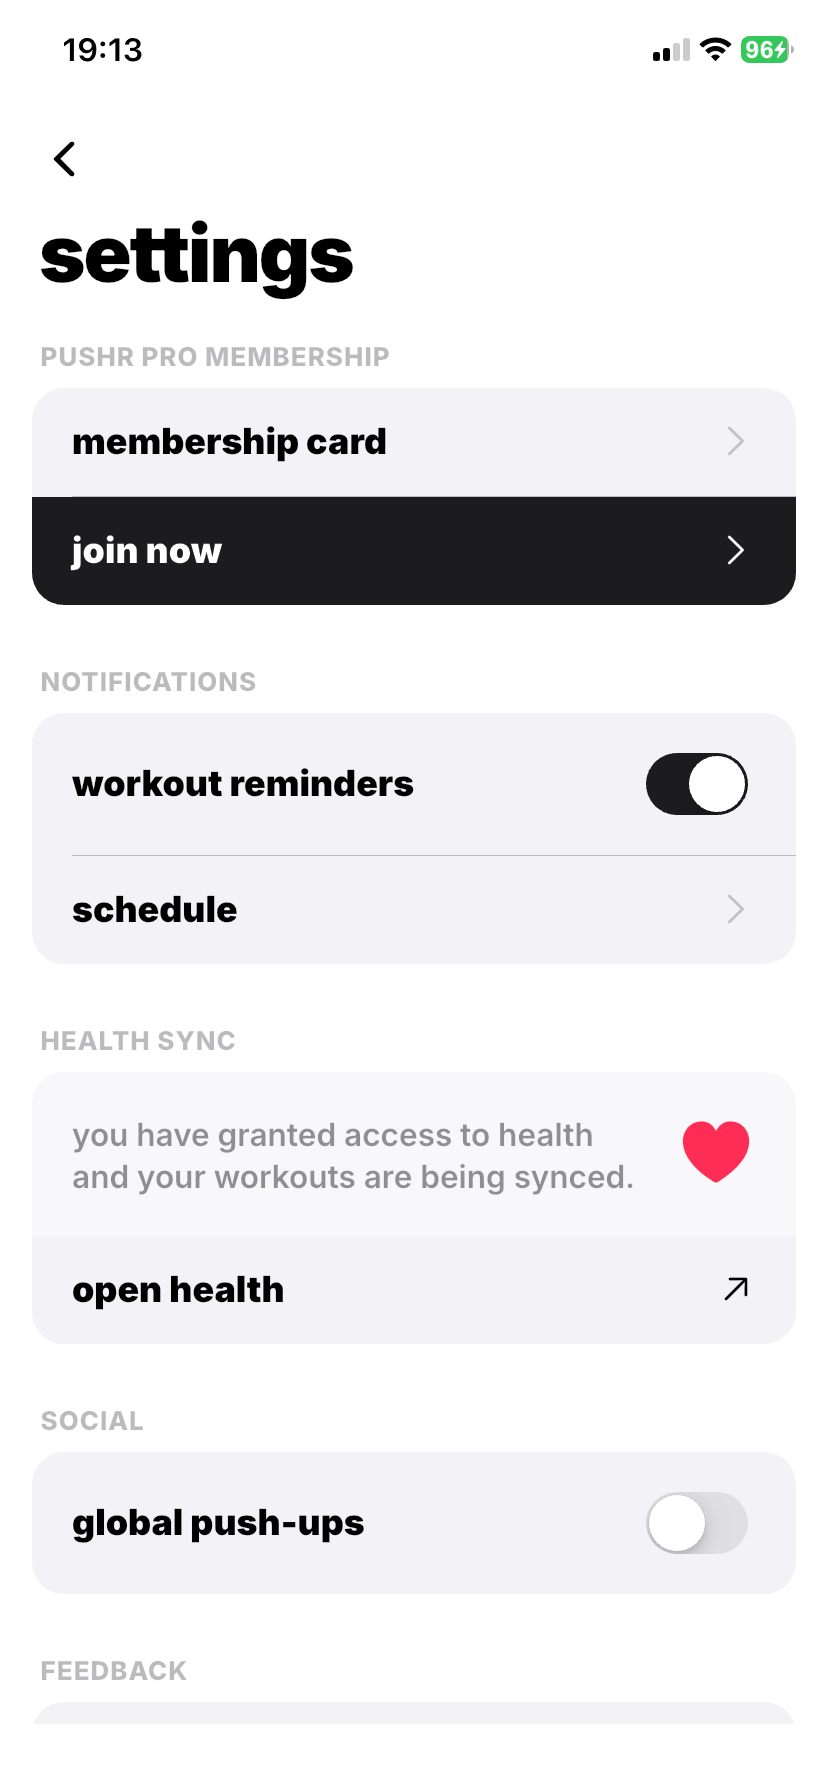
\includegraphics[height=9.5cm]{push_up/IMG_6876.PNG}
        \caption{Giao diện cấu hình và đồng bộ Health Sync.}
        \label{fig:pushup_settings}
    \end{minipage}
\end{figure}

\newpage
\begin{figure}[htbp]
    \centering
    \begin{minipage}{0.45\textwidth}
        \centering
        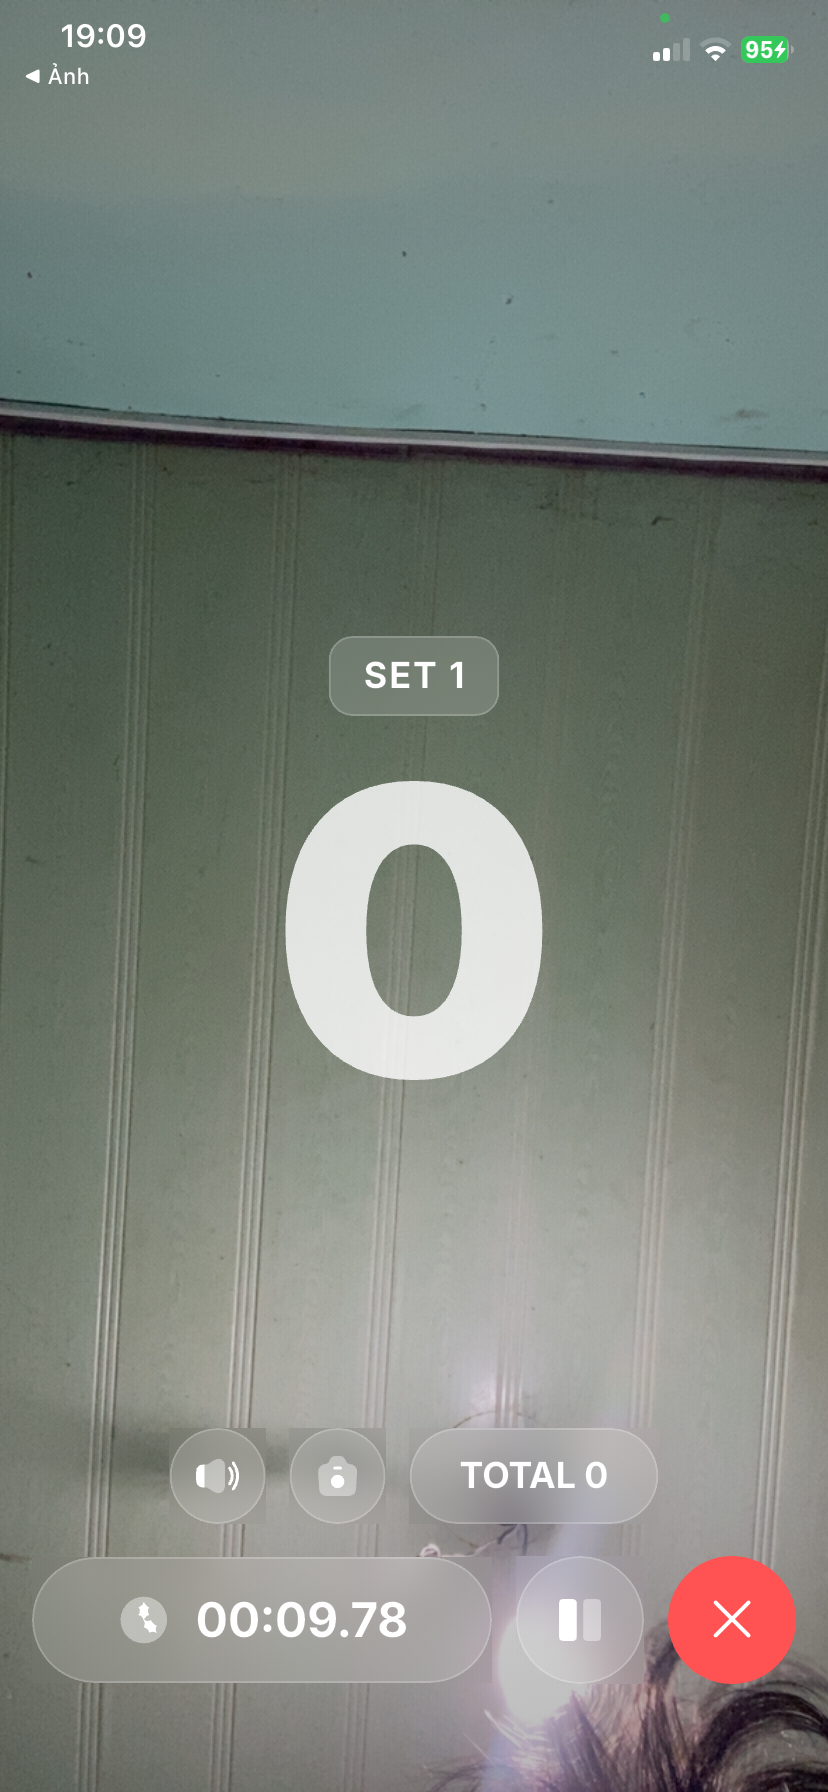
\includegraphics[height=9.5cm]{push_up/IMG_6871.PNG}
        \caption{Giao diện buổi tập hít đất (Start Workout).}
        \label{fig:pushup_work}
    \end{minipage}
    \hfill
    \begin{minipage}{0.45\textwidth}
        \centering
        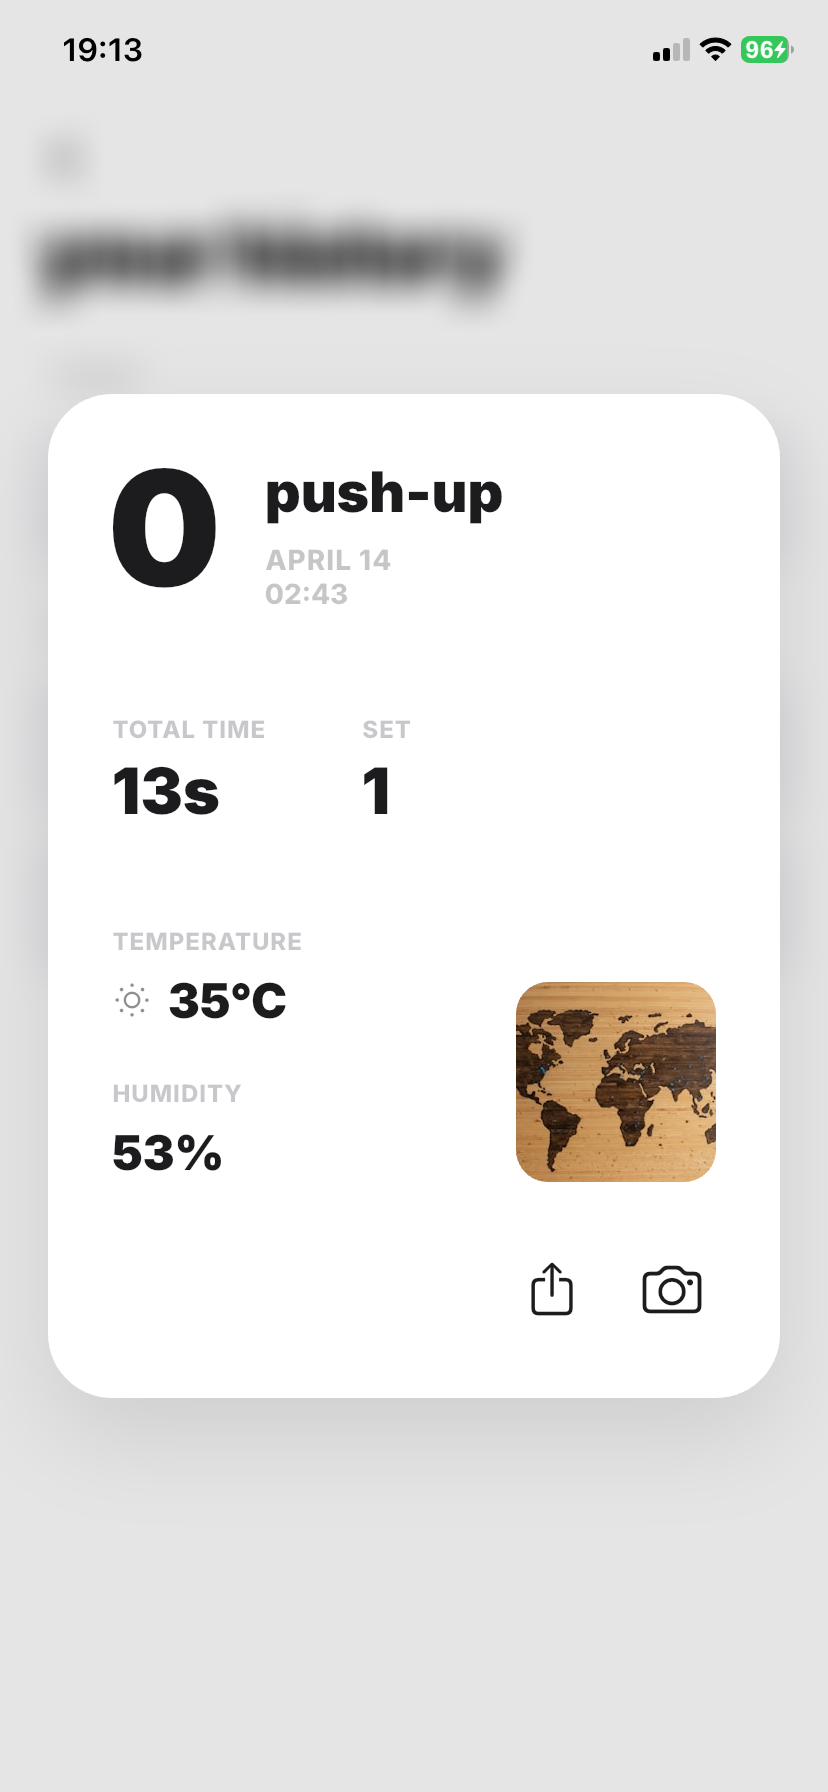
\includegraphics[height=9.5cm]{push_up/IMG_6875.PNG}
        \caption{Thẻ báo cáo chia sẻ buổi tập (Workout Report).}
        \label{fig:pushup_report}
    \end{minipage}
\end{figure}

\newpage
\begin{figure}[htbp]
    \centering
    \begin{minipage}{0.45\textwidth}
        \centering
        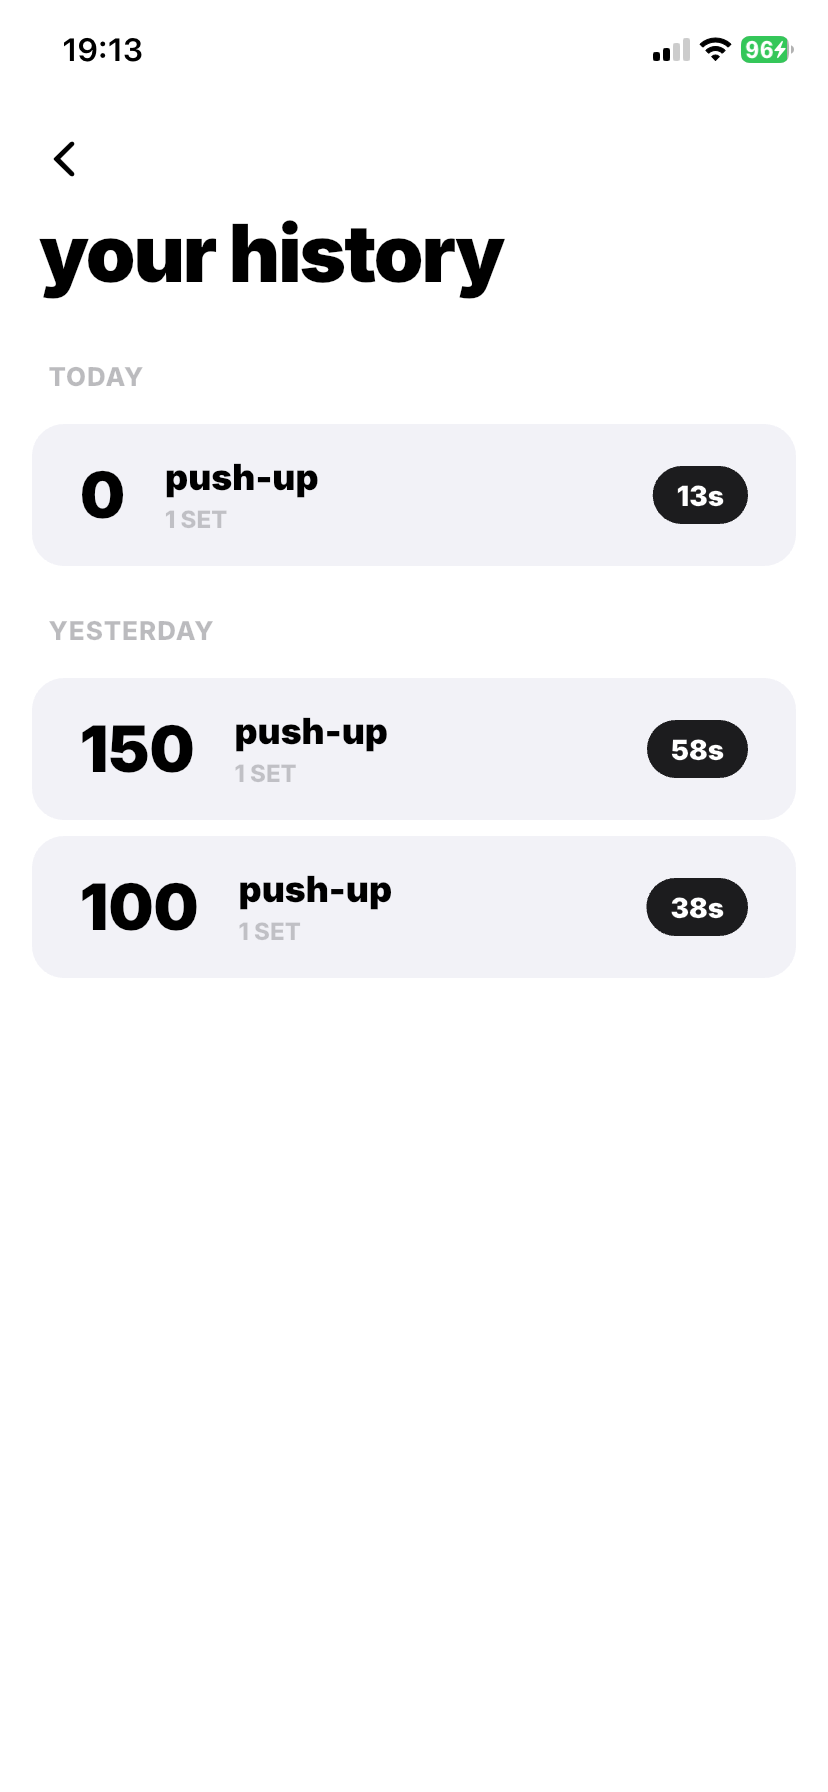
\includegraphics[height=9.5cm]{push_up/IMG_6874.PNG}
        \caption{Giao diện quản lý lịch sử các buổi tập (History).}
        \label{fig:pushup_history}
    \end{minipage}
    \hfill
    \begin{minipage}{0.45\textwidth}
        \centering
        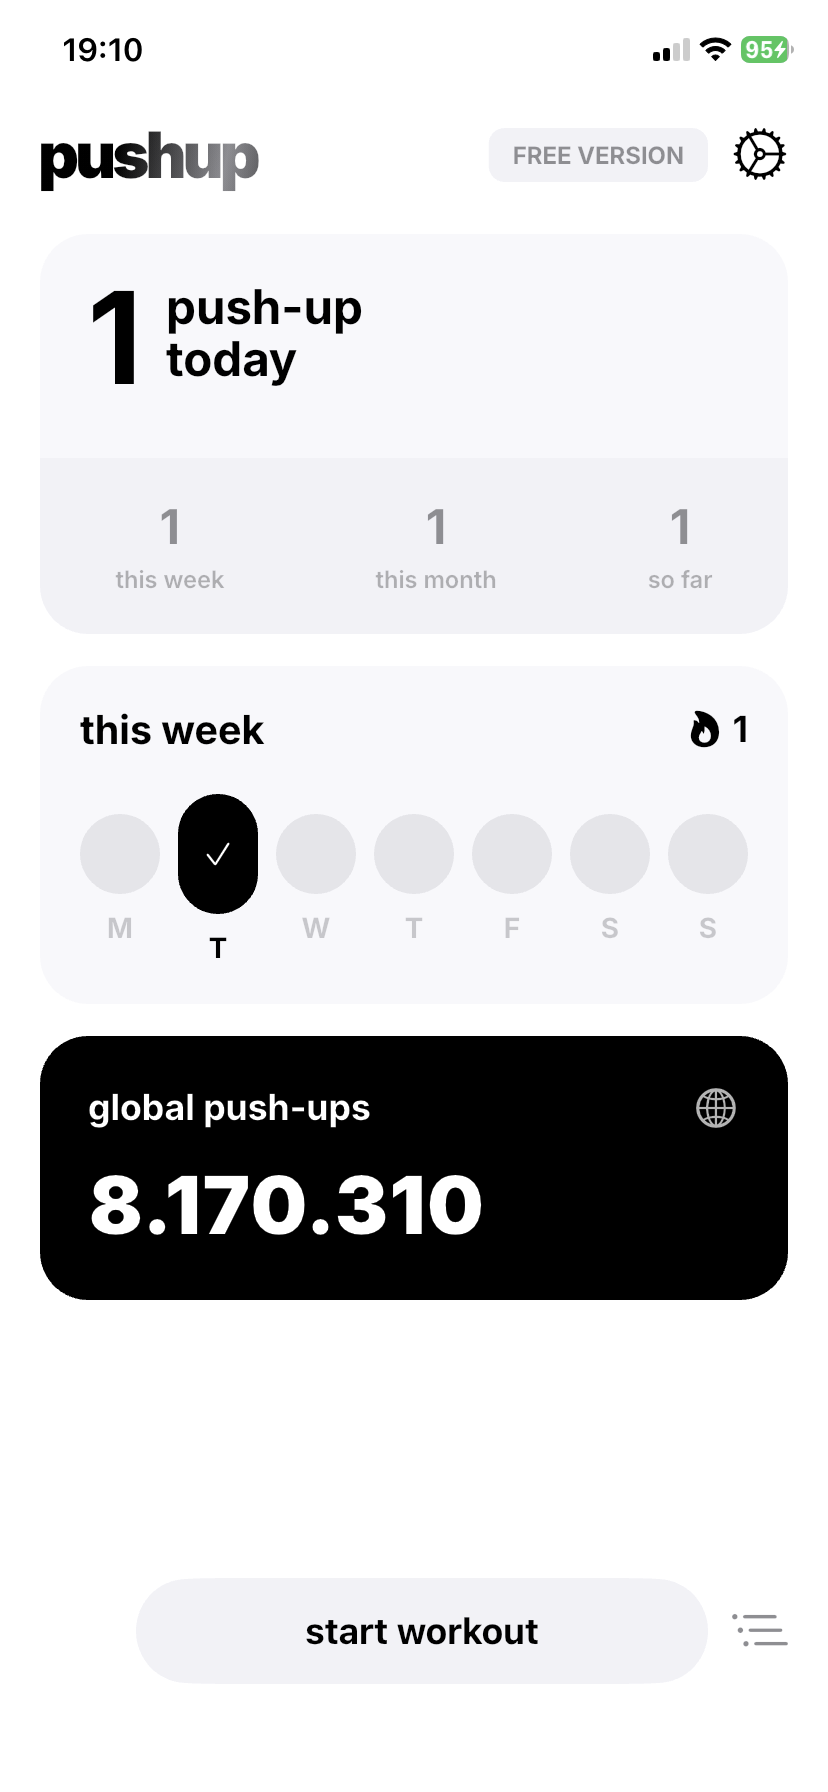
\includegraphics[height=9.5cm]{push_up/IMG_6873.PNG}
        \caption{Dashboard ghi nhận hít đất thành công đầu tiên.}
        \label{fig:pushup_success}
    \end{minipage}
\end{figure}

\newpage
\subsection*{Phần 3: Dự án PDF Converter \& Scanner (Giai đoạn 3)}
Ứng dụng quét tài liệu chuyên nghiệp và chuyển đổi đa định dạng ngoại tuyến:

\subsubsection*{3.1. Màn hình Convert và luồng nhập liệu đa nguồn}
\begin{figure}[htbp]
    \centering
    \begin{minipage}{0.45\textwidth}
        \centering
        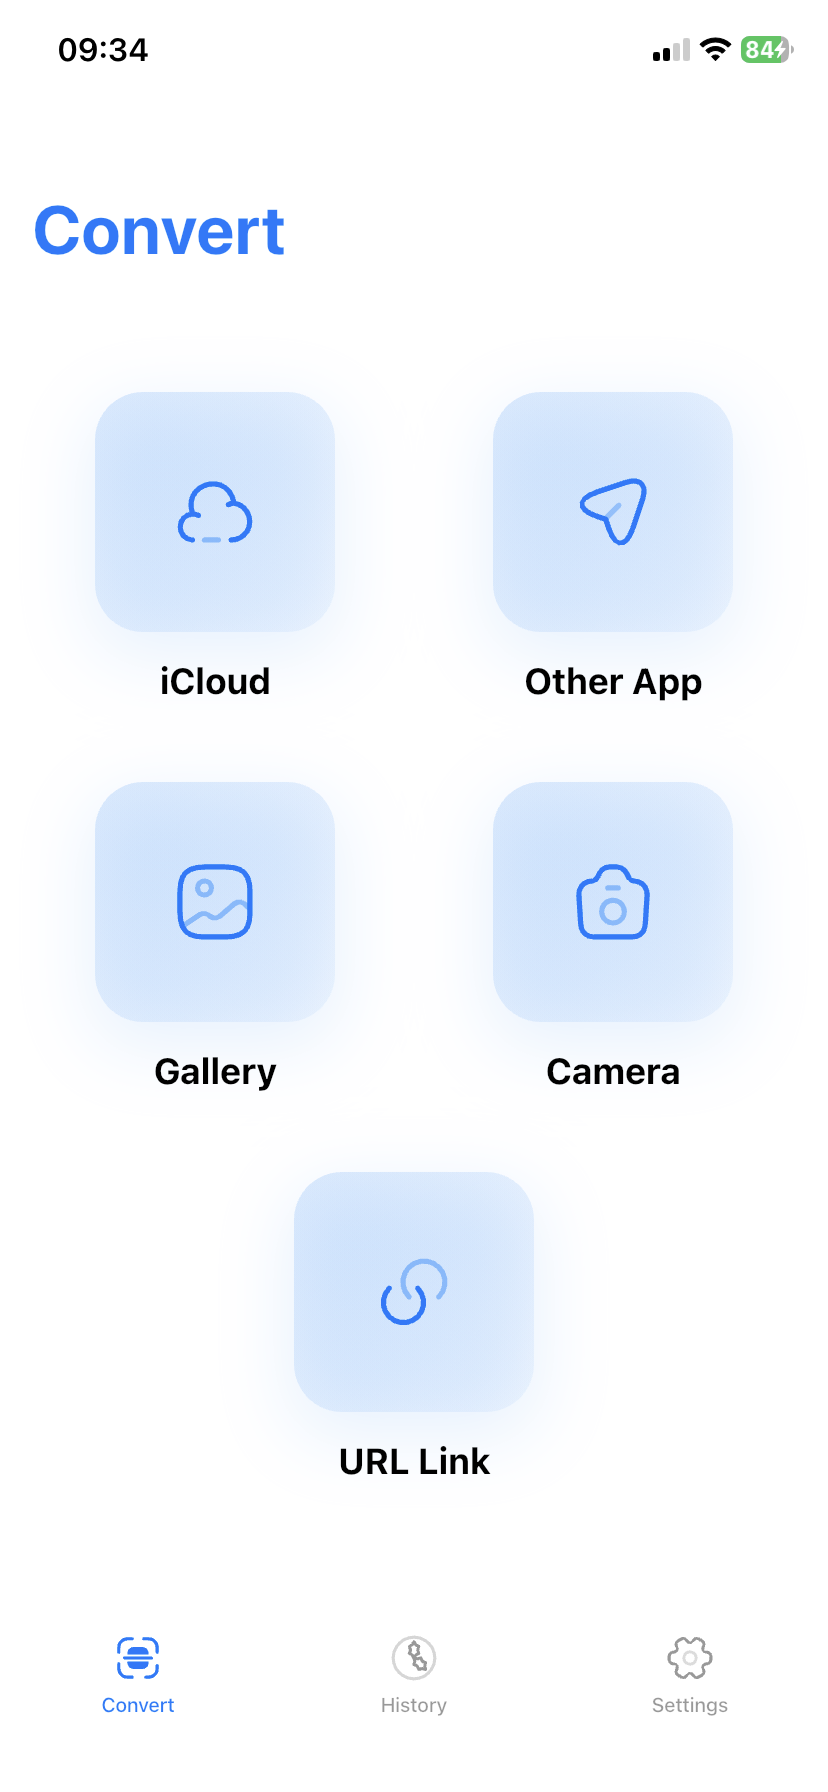
\includegraphics[height=9.5cm]{features/IMG_7576.PNG}
        \caption{Màn hình Convert chính với 5 nguồn nhập liệu: iCloud, Other App, Gallery, Camera, URL Link.}
        \label{fig:pdf_convert_home}
    \end{minipage}
    \hfill
    \begin{minipage}{0.45\textwidth}
        \centering
        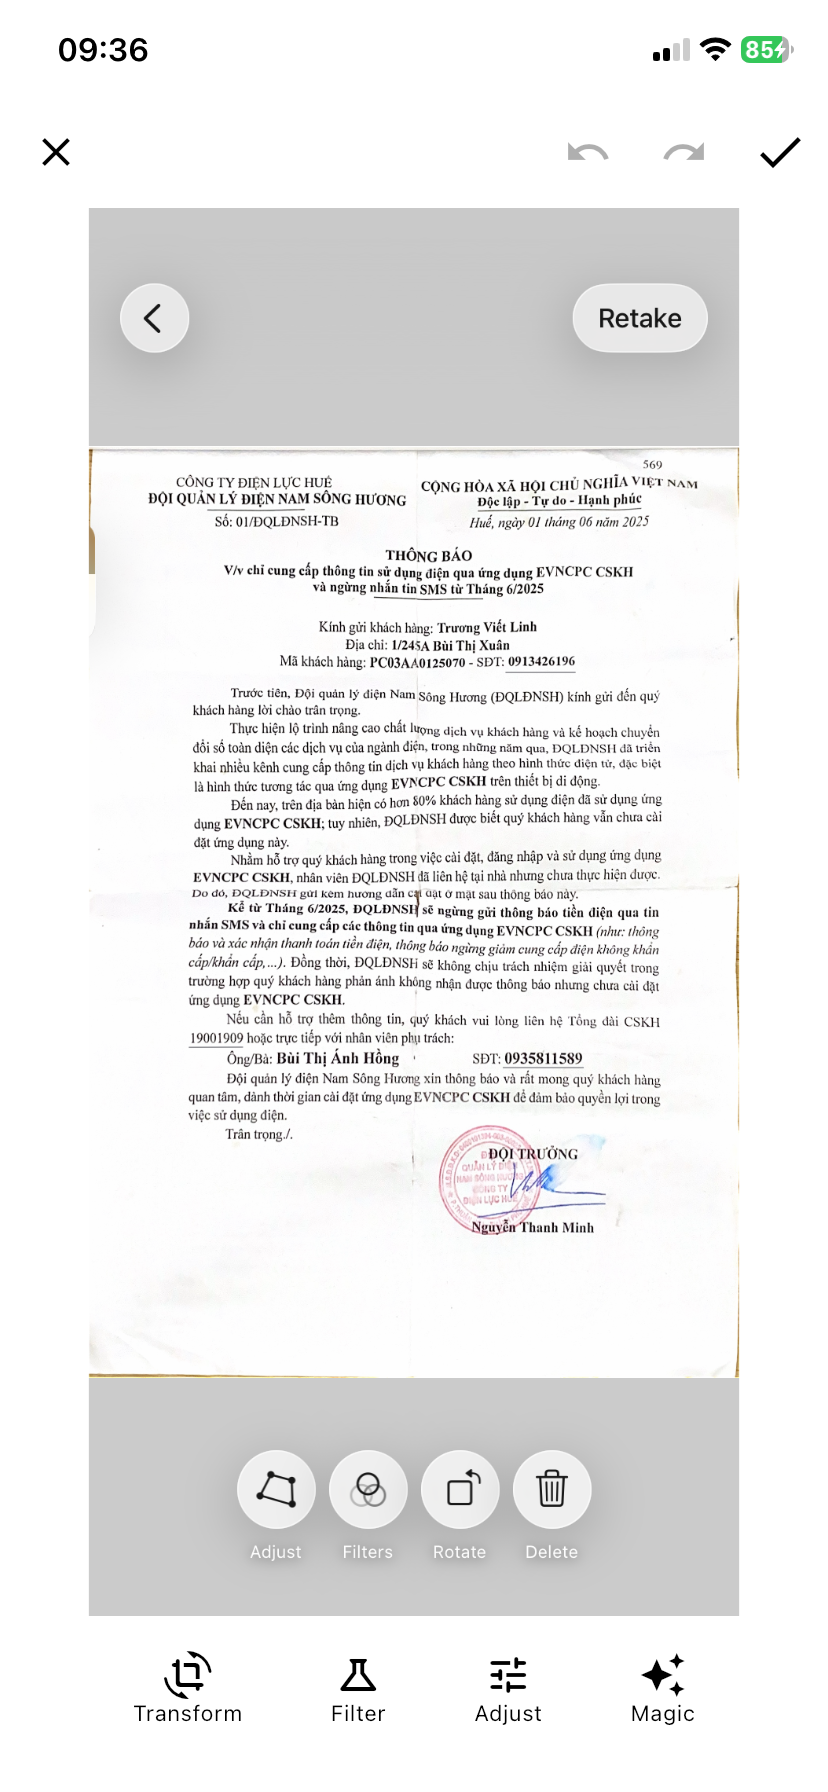
\includegraphics[height=9.5cm]{features/IMG_7592.PNG}
        \caption{Popup ``Enter URL'': nhập liên kết URL để tải và chuyển đổi tài liệu trực tiếp từ Internet.}
        \label{fig:pdf_url}
    \end{minipage}
\end{figure}

\begin{figure}[htbp]
    \centering
    \begin{minipage}{0.45\textwidth}
        \centering
        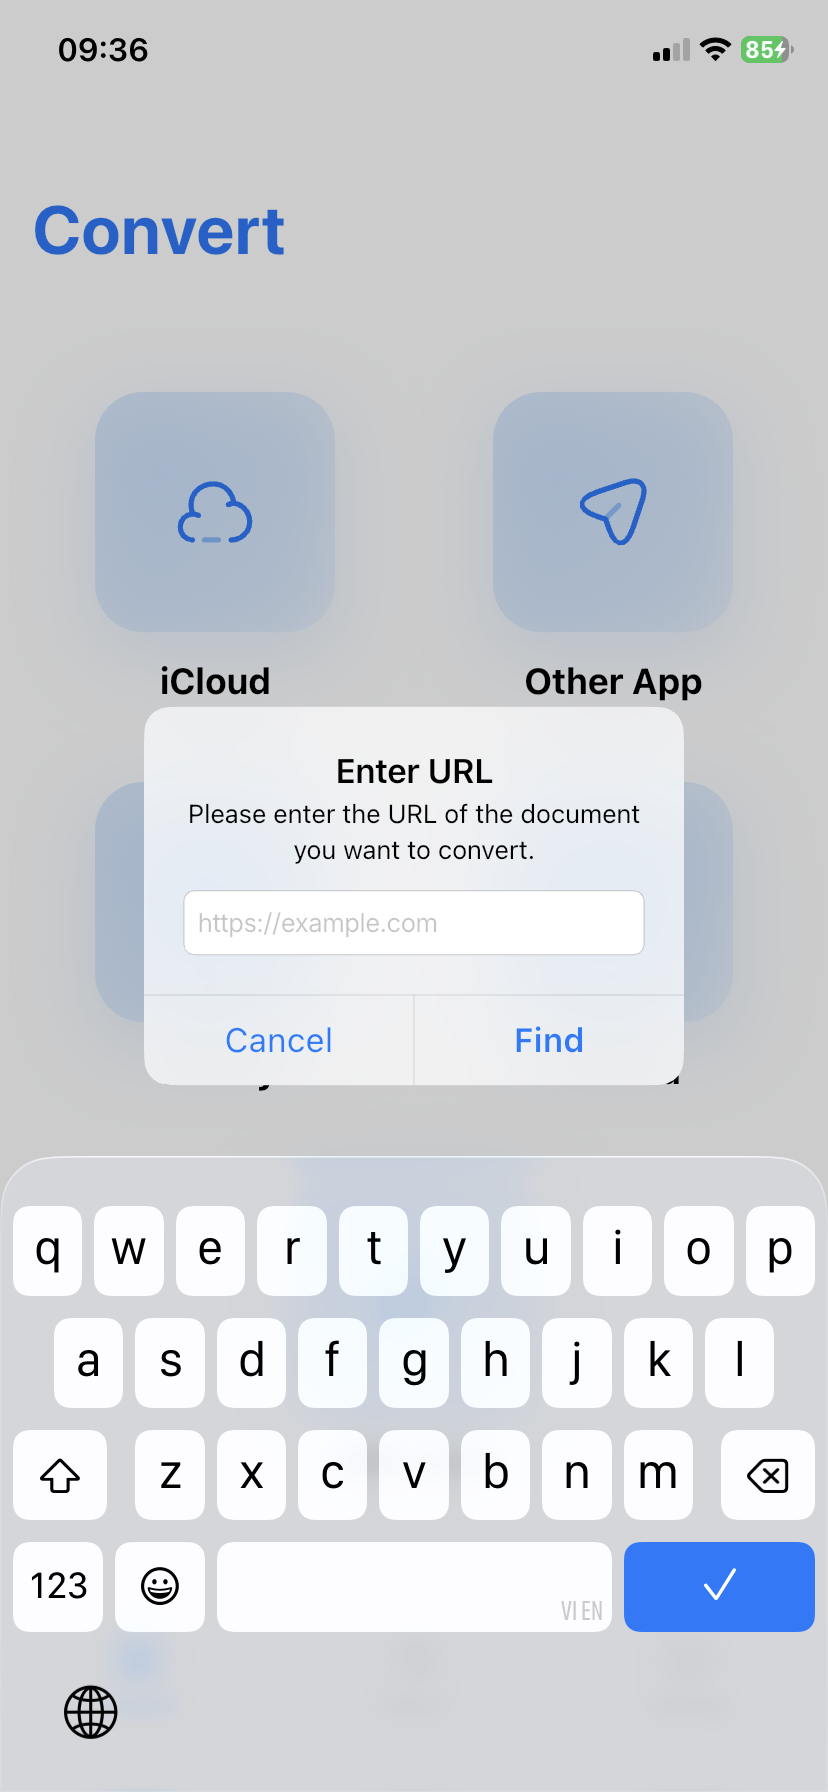
\includegraphics[height=9.5cm]{features/IMG_7593.PNG}
        \caption{Màn hình iCloud Picker: chọn file từ iCloud Drive (Gần đây, Được chia sẻ, Duyệt) với thanh tìm kiếm.}
        \label{fig:pdf_icloud}
    \end{minipage}
    \hfill
    \begin{minipage}{0.45\textwidth}
        \centering
        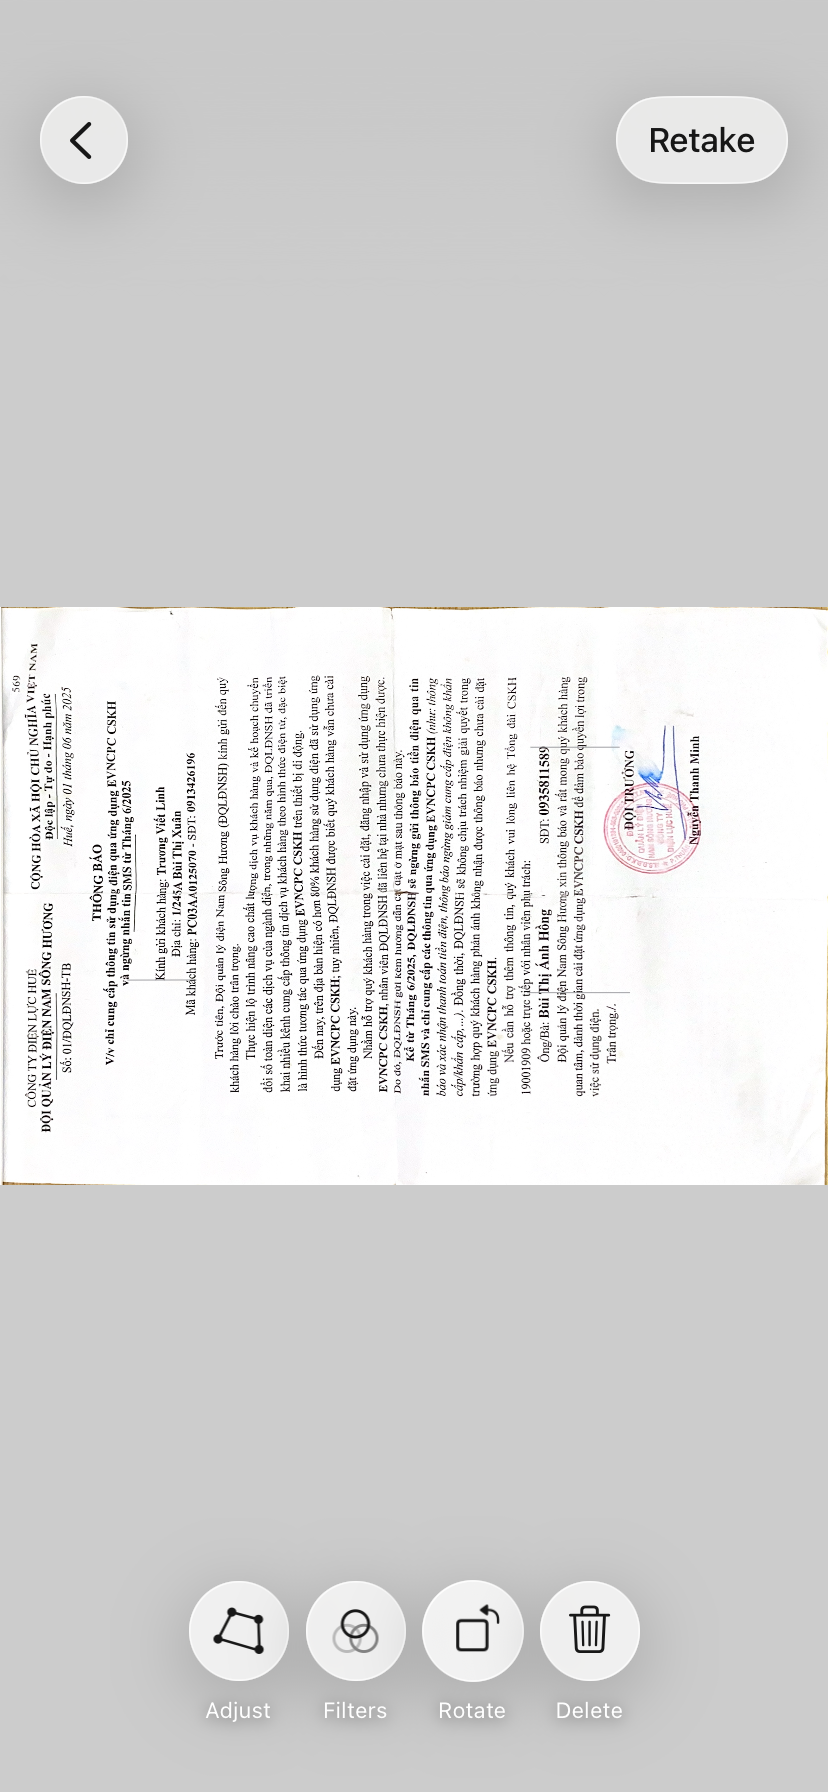
\includegraphics[height=9.5cm]{features/IMG_7584.PNG}
        \caption{Màn hình New Conversion: file đã chọn, định dạng đích .pdf, PDF Settings chất lượng 90\%, nút Convert.}
        \label{fig:pdf_new_conversion}
    \end{minipage}
\end{figure}

\newpage
\subsubsection*{3.2. Quét tài liệu qua Camera và hiệu chỉnh phối cảnh}
\begin{figure}[htbp]
    \centering
    \begin{minipage}{0.45\textwidth}
        \centering
        \includegraphics[height=9.5cm]{features/IMG_7580.PNG}
        \caption{Giao diện Camera Scanner: quét tài liệu trực tiếp với thanh điều khiển Flash, Filters, Shutter.}
        \label{fig:pdf_camera}
    \end{minipage}
    \hfill
    \begin{minipage}{0.45\textwidth}
        \centering
        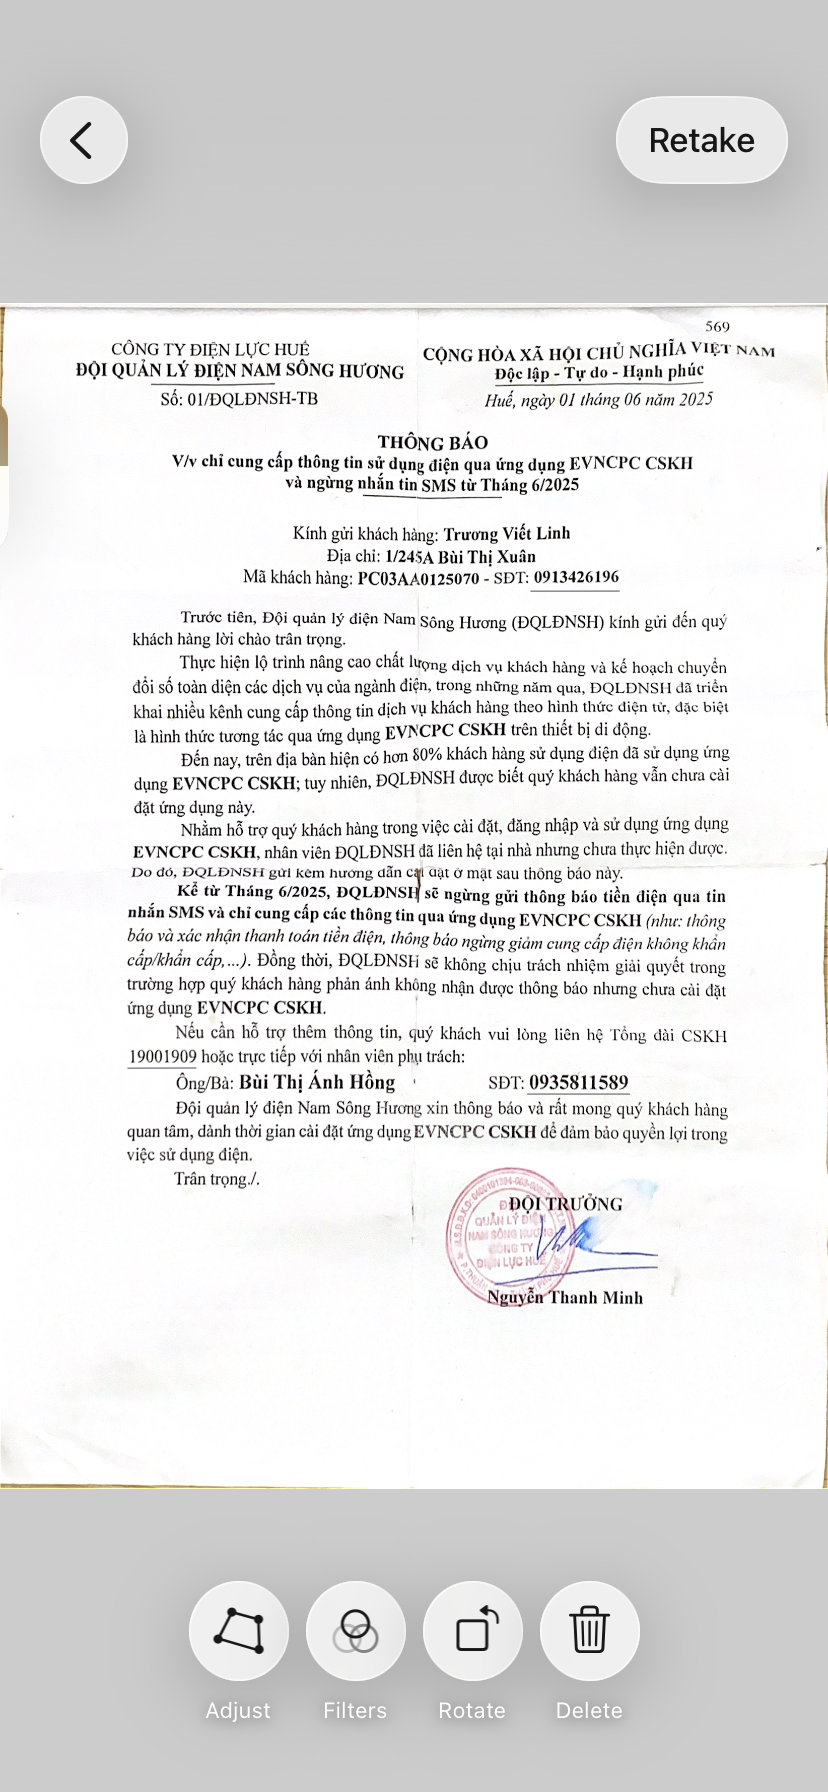
\includegraphics[height=9.5cm]{features/IMG_7581.PNG}
        \caption{Màn hình Perspective Crop: hiệu chỉnh phối cảnh tài liệu với 4 đỉnh tương tác và toolbar Adjust/Filters/Rotate/Delete.}
        \label{fig:pdf_crop}
    \end{minipage}
\end{figure}

\begin{figure}[htbp]
    \centering
    \begin{minipage}{0.45\textwidth}
        \centering
        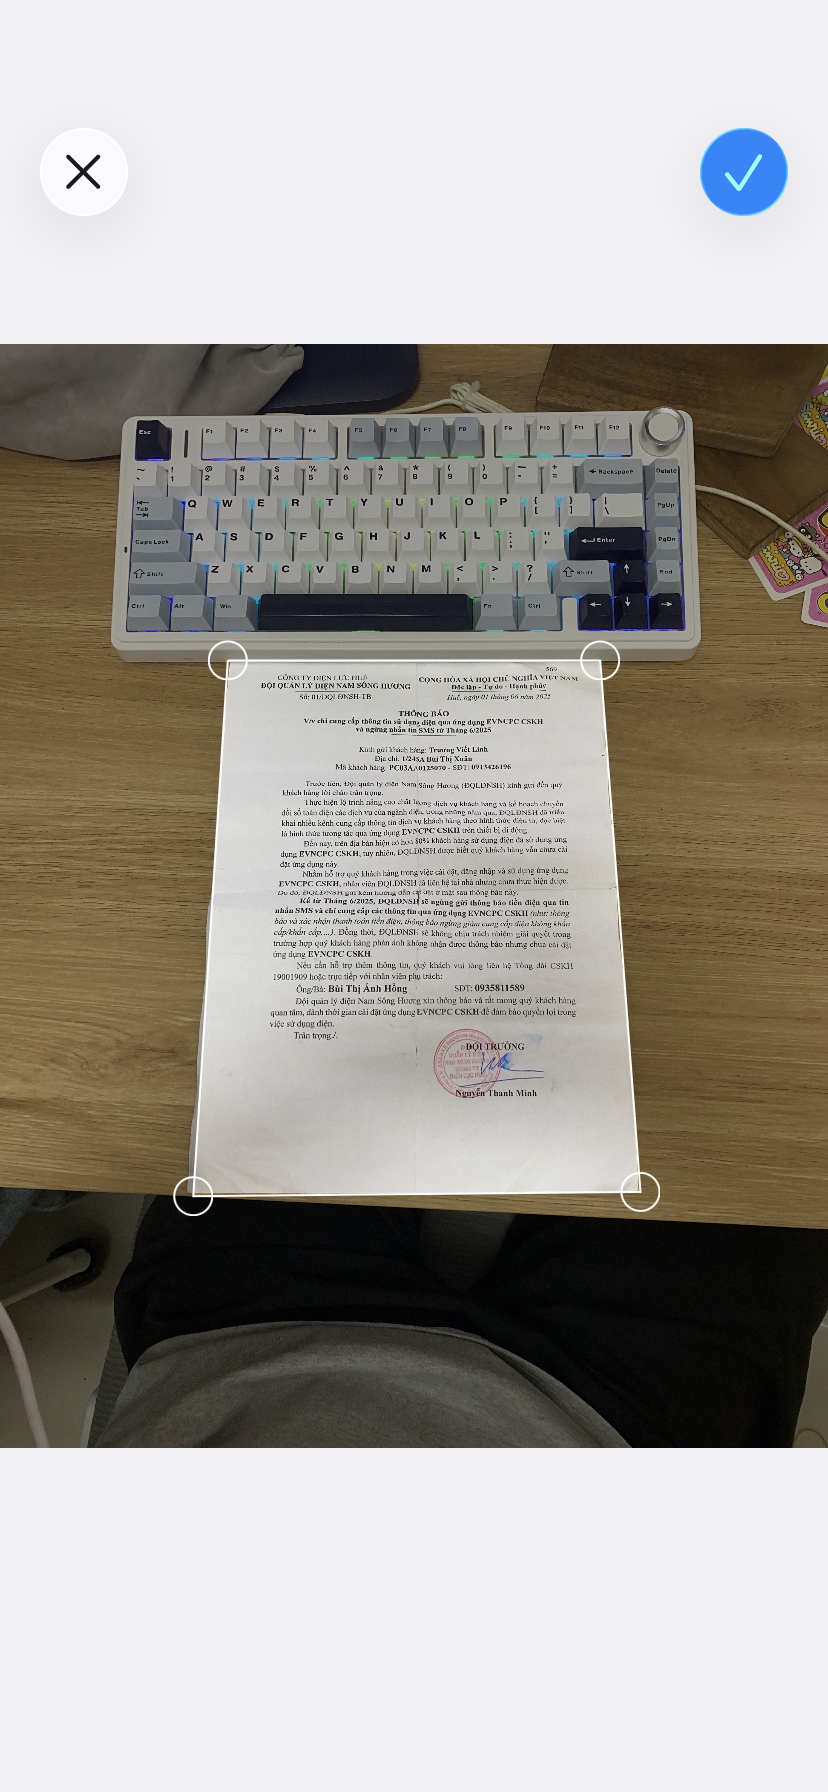
\includegraphics[height=9.5cm]{features/IMG_7582.PNG}
        \caption{Picker chọn bộ lọc tài liệu: Black \& White, Grayscale, Color, Photo để chuẩn hóa ảnh quét.}
        \label{fig:pdf_filter_picker}
    \end{minipage}
    \hfill
    \begin{minipage}{0.45\textwidth}
        \centering
        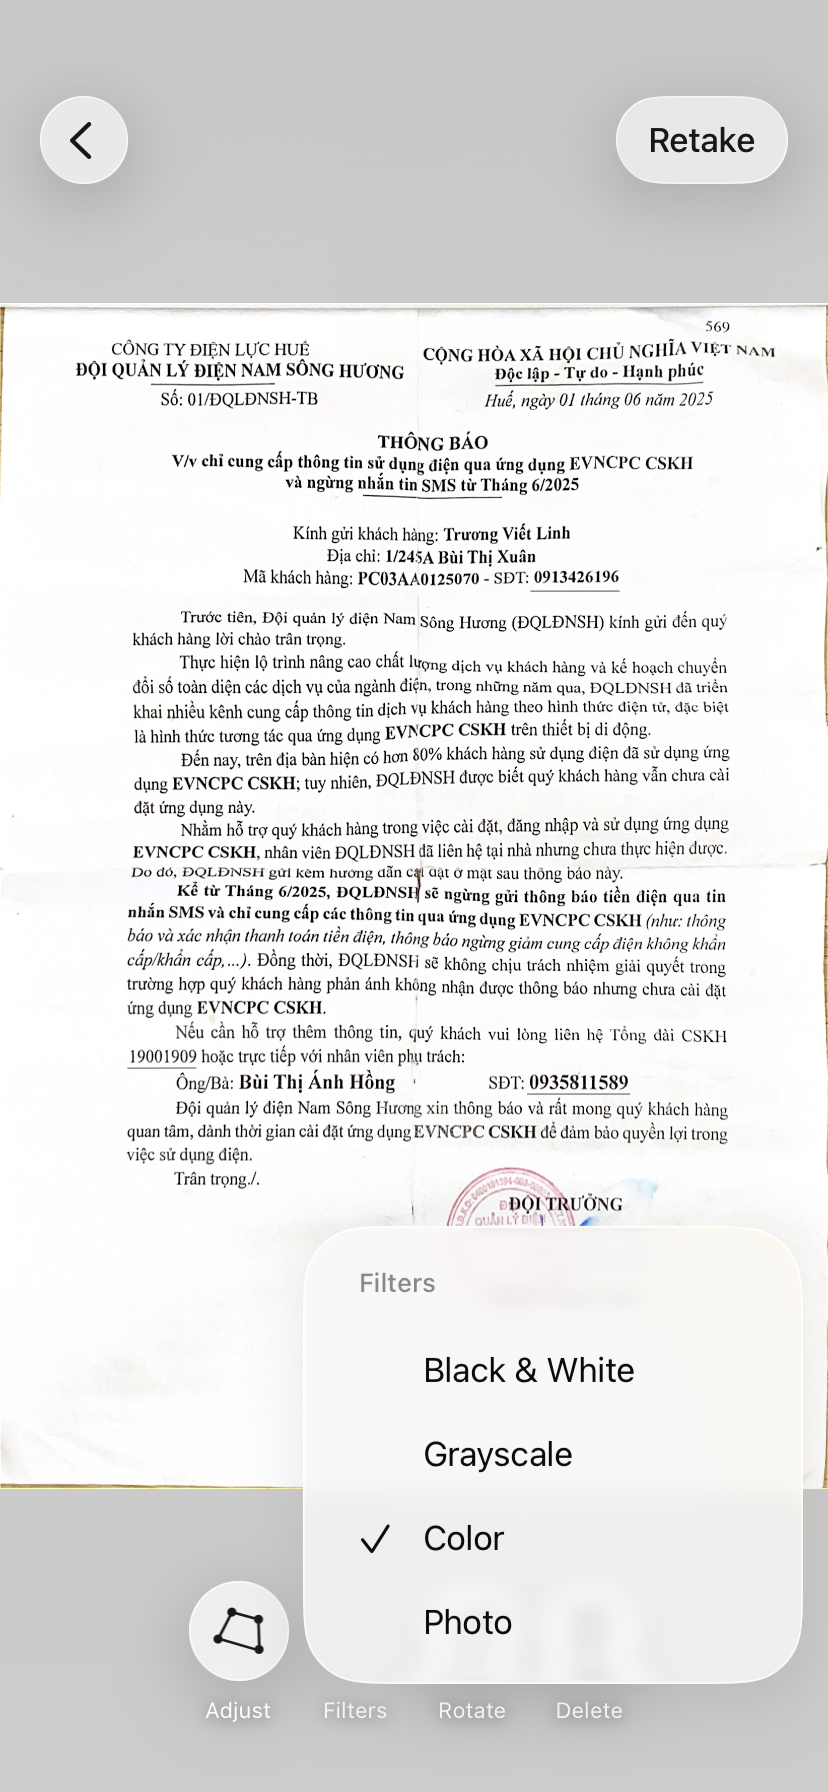
\includegraphics[height=9.5cm]{features/IMG_7583.PNG}
        \caption{Kết quả sau khi xoay tài liệu quét sang chế độ ngang (Rotate), sẵn sàng xác nhận lưu.}
        \label{fig:pdf_rotated}
    \end{minipage}
\end{figure}

\newpage
\subsubsection*{3.3. Bộ chỉnh sửa ảnh nâng cao và chọn định dạng đích}
\begin{figure}[htbp]
    \centering
    \begin{minipage}{0.45\textwidth}
        \centering
        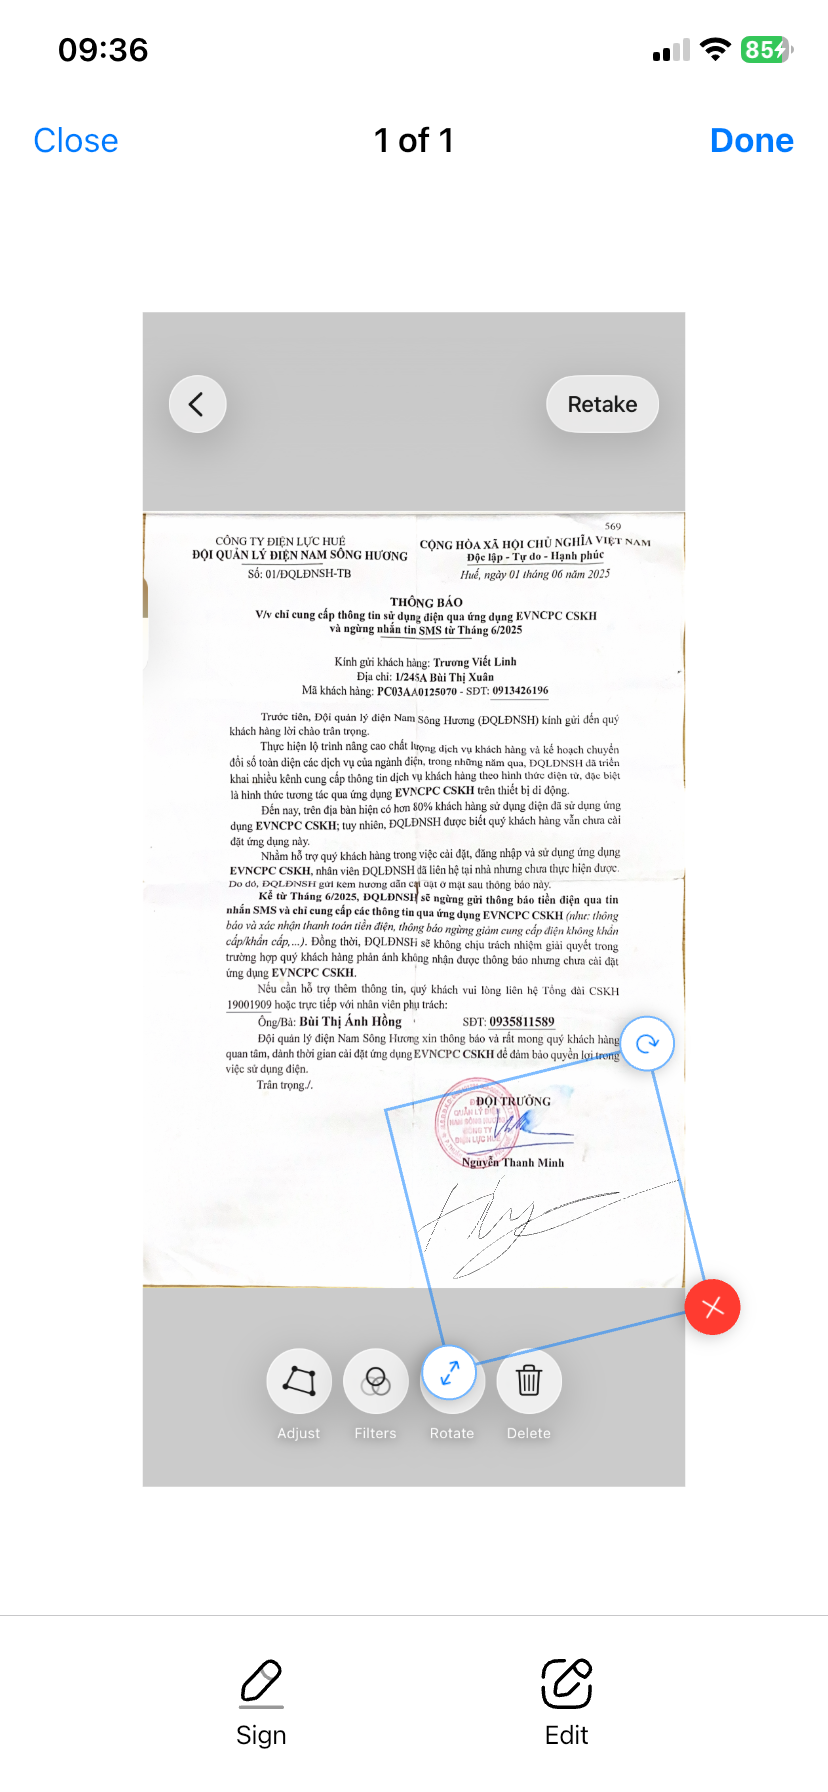
\includegraphics[height=9.5cm]{features/IMG_7591.PNG}
        \caption{Bộ pro\_image\_editor tích hợp sâu với 4 công cụ chỉnh sửa: Transform, Filter, Adjust, Magic.}
        \label{fig:pdf_pro_editor}
    \end{minipage}
    \hfill
    \begin{minipage}{0.45\textwidth}
        \centering
        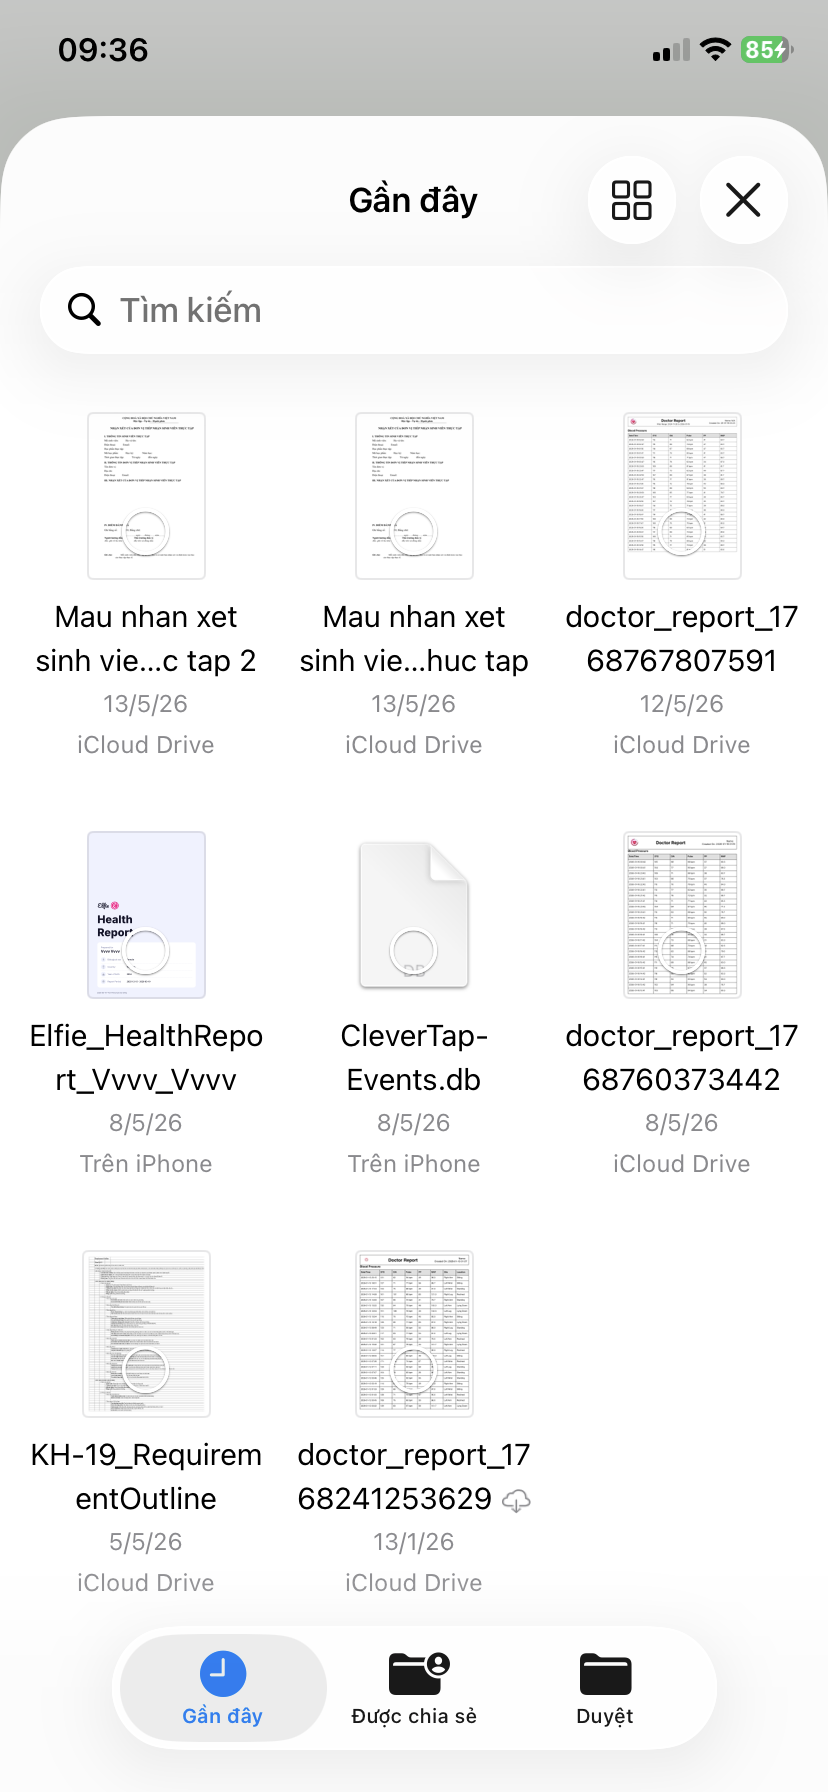
\includegraphics[height=9.5cm]{features/IMG_7594.PNG}
        \caption{Màn hình Target extension: chọn định dạng đích .pdf, .doc, .docx, .jpg, .png, .epub, .txt, .xls, .xlsx, .mobi, .ppt.}
        \label{fig:pdf_target_ext}
    \end{minipage}
\end{figure}

\begin{figure}[htbp]
    \centering
    \begin{minipage}{0.45\textwidth}
        \centering
        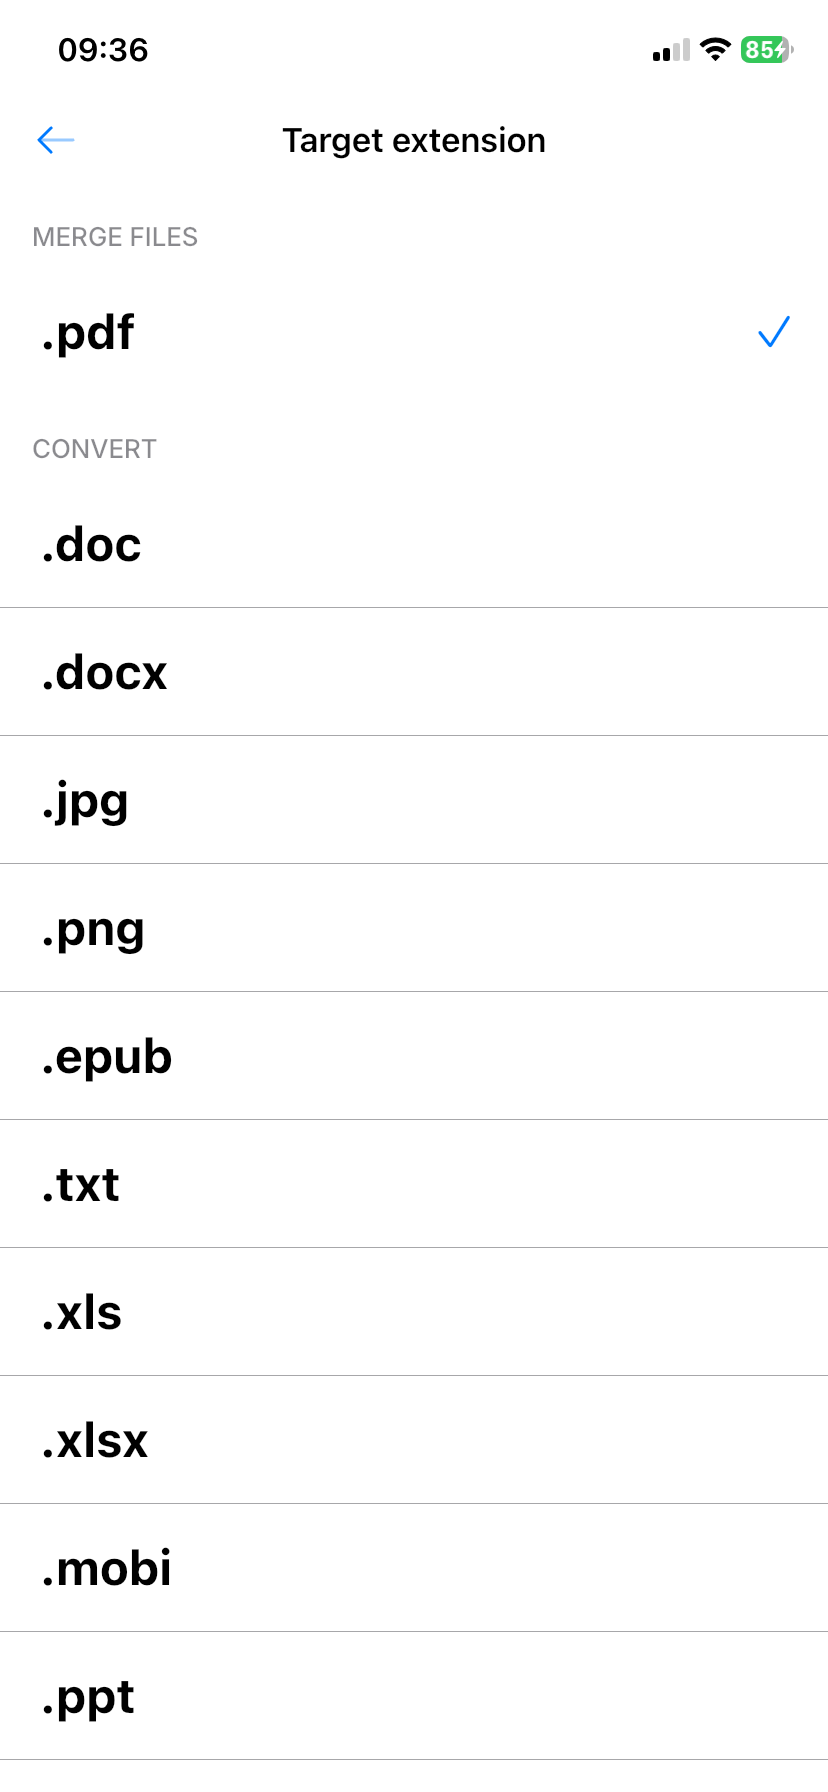
\includegraphics[height=9.5cm]{features/IMG_7595.PNG}
        \caption{Màn hình Target extension đầy đủ: nhóm Merge Files (.pdf) và toàn bộ định dạng Convert đa dạng.}
        \label{fig:pdf_formats_full}
    \end{minipage}
    \hfill
    \begin{minipage}{0.45\textwidth}
        \centering
        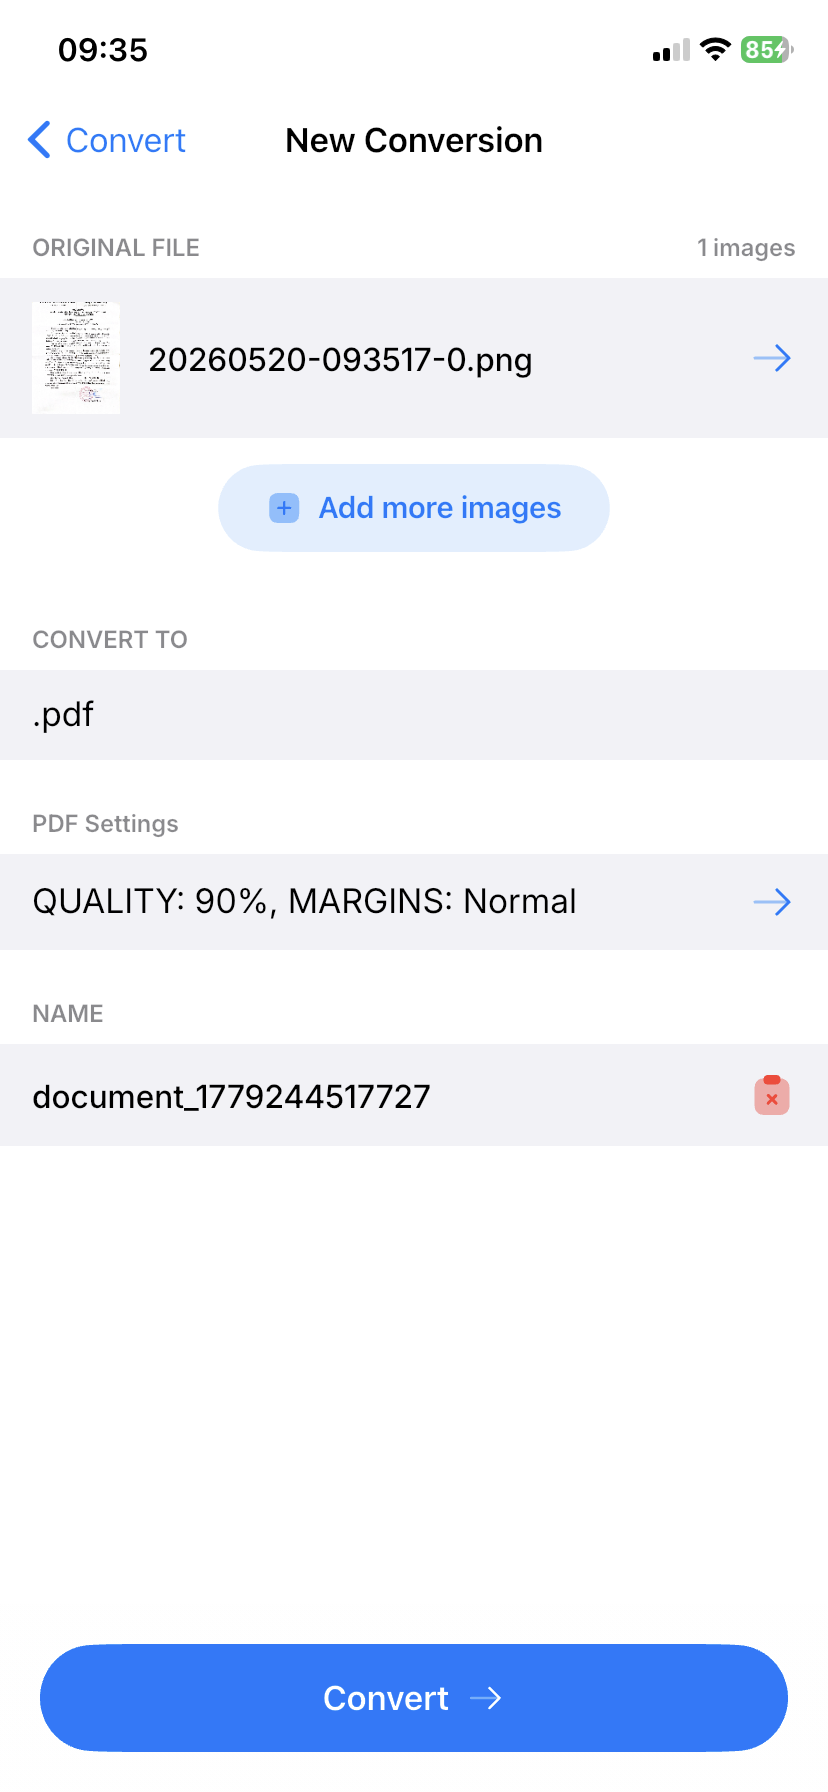
\includegraphics[height=9.5cm]{features/IMG_7585.PNG}
        \caption{Màn hình ``Creating PDF'': Circular Progress Indicator hiển thị 6\% với thông điệp ``Optimizing PDF...''}
        \label{fig:pdf_progress}
    \end{minipage}
\end{figure}

\newpage
\subsubsection*{3.4. Xuất tệp PDF và xem trước tài liệu}
\begin{figure}[htbp]
    \centering
    \begin{minipage}{0.45\textwidth}
        \centering
        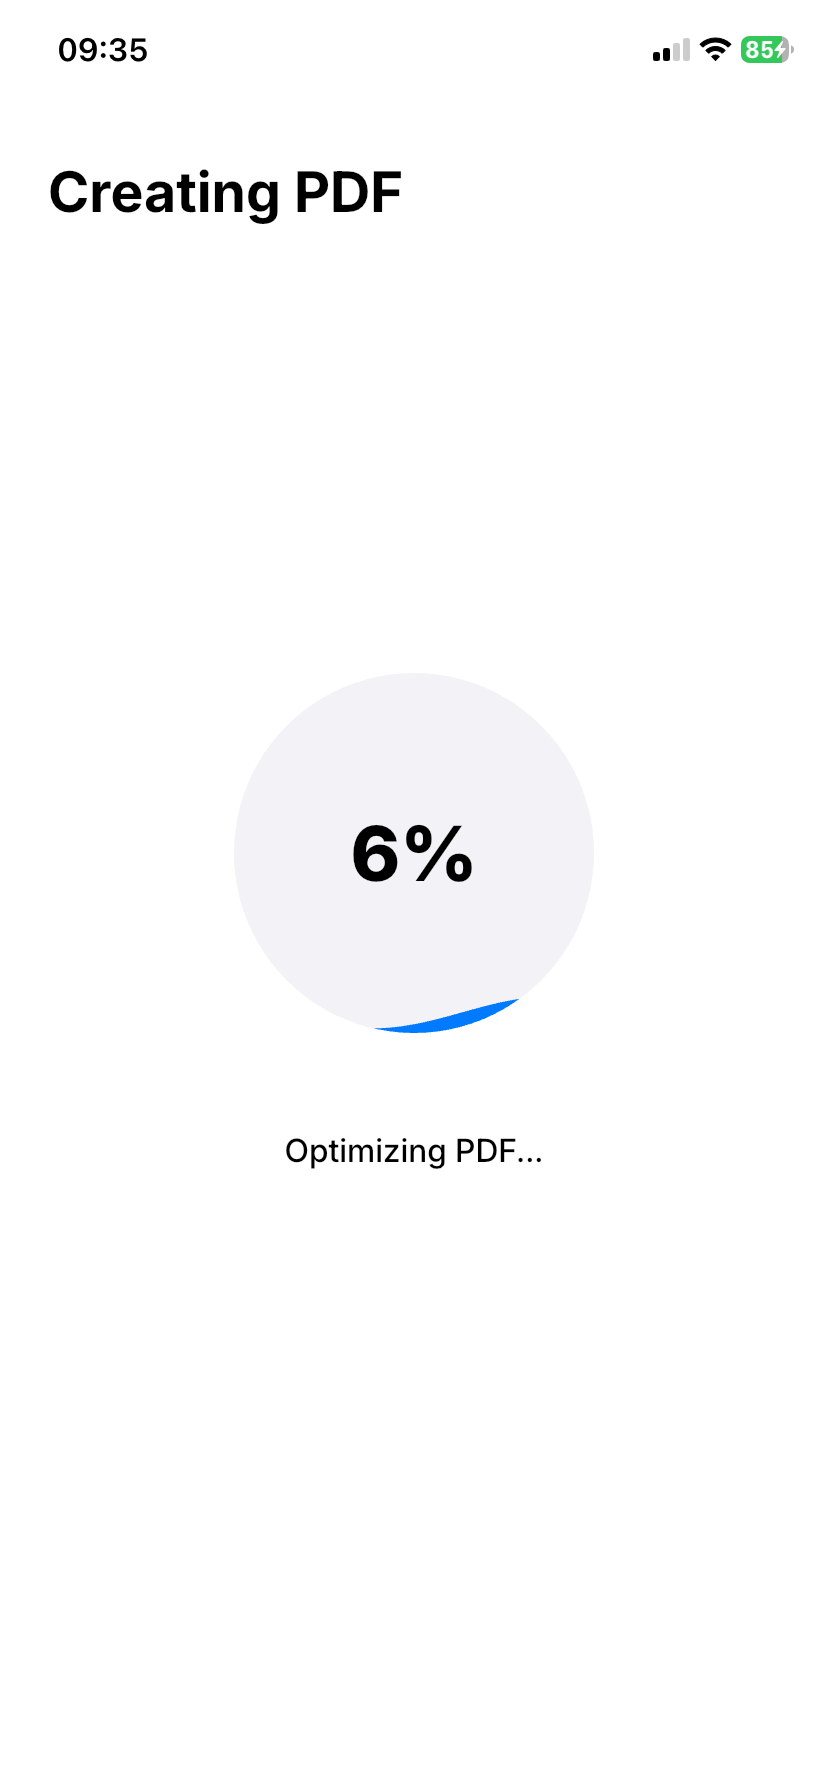
\includegraphics[height=9.5cm]{features/IMG_7586.PNG}
        \caption{Màn hình ``PDF Exported Successfully'' và iOS Share Sheet: chia sẻ qua AirDrop, Mail, Zalo và ứng dụng khác.}
        \label{fig:pdf_exported}
    \end{minipage}
    \hfill
    \begin{minipage}{0.45\textwidth}
        \centering
        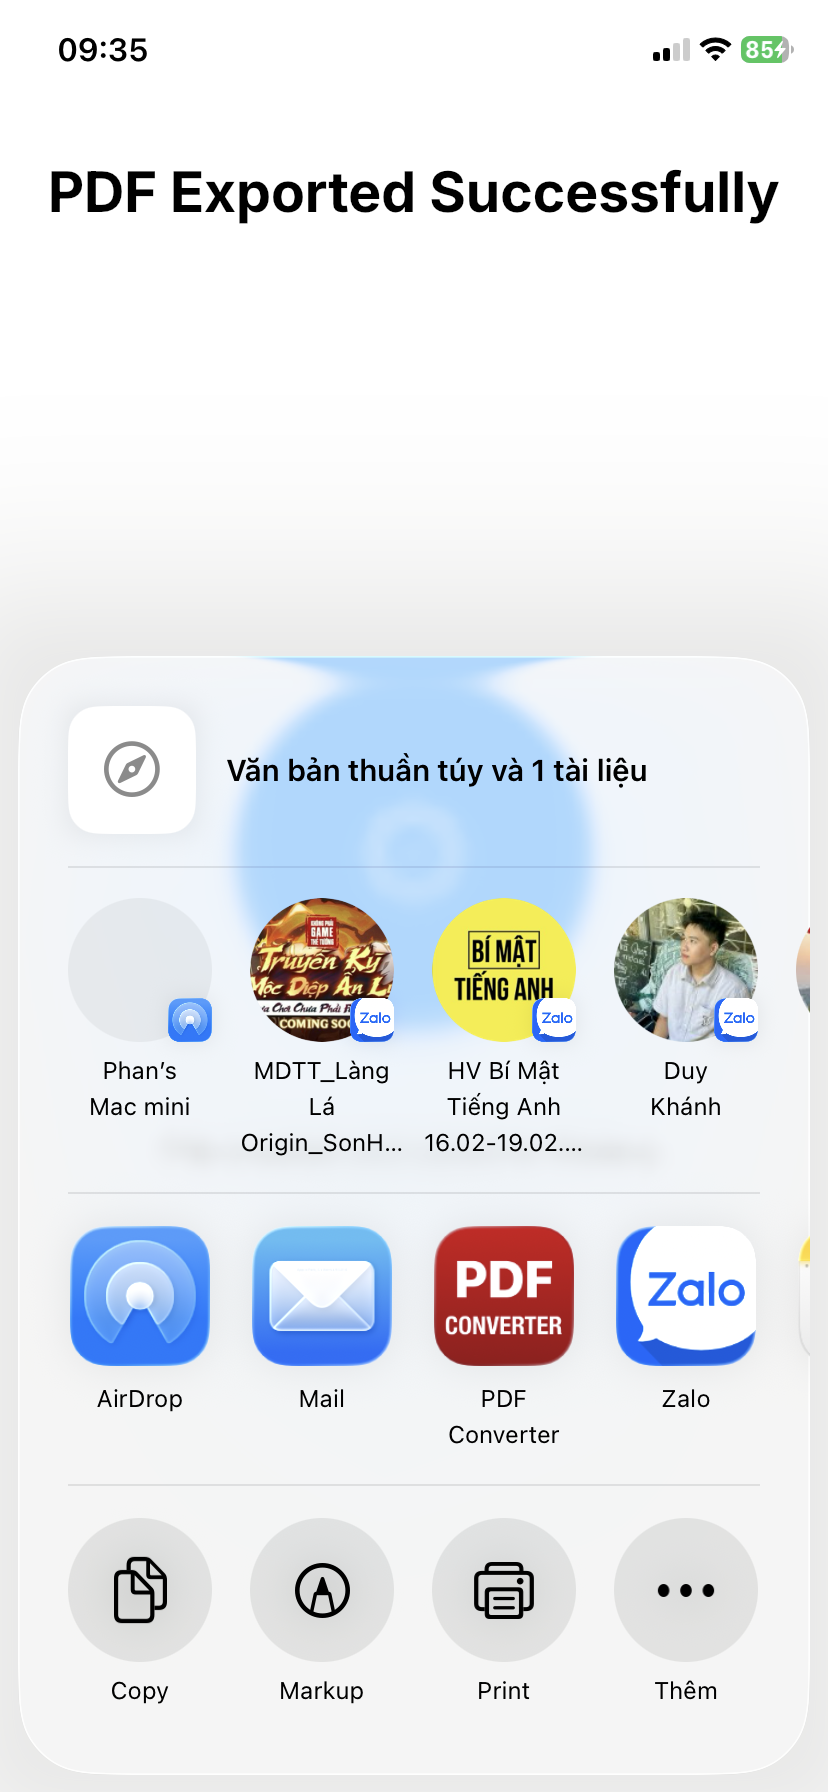
\includegraphics[height=9.5cm]{features/IMG_7587.PNG}
        \caption{Màn hình xem trước PDF sau chuyển đổi (1 of 1) với nút Sign (Ký chữ ký) và Edit (Chỉnh sửa ảnh).}
        \label{fig:pdf_preview}
    \end{minipage}
\end{figure}

\newpage
\subsubsection*{3.5. Phân hệ Chữ ký tay số (Digital Signature)}
\begin{figure}[htbp]
    \centering
    \begin{minipage}{0.45\textwidth}
        \centering
        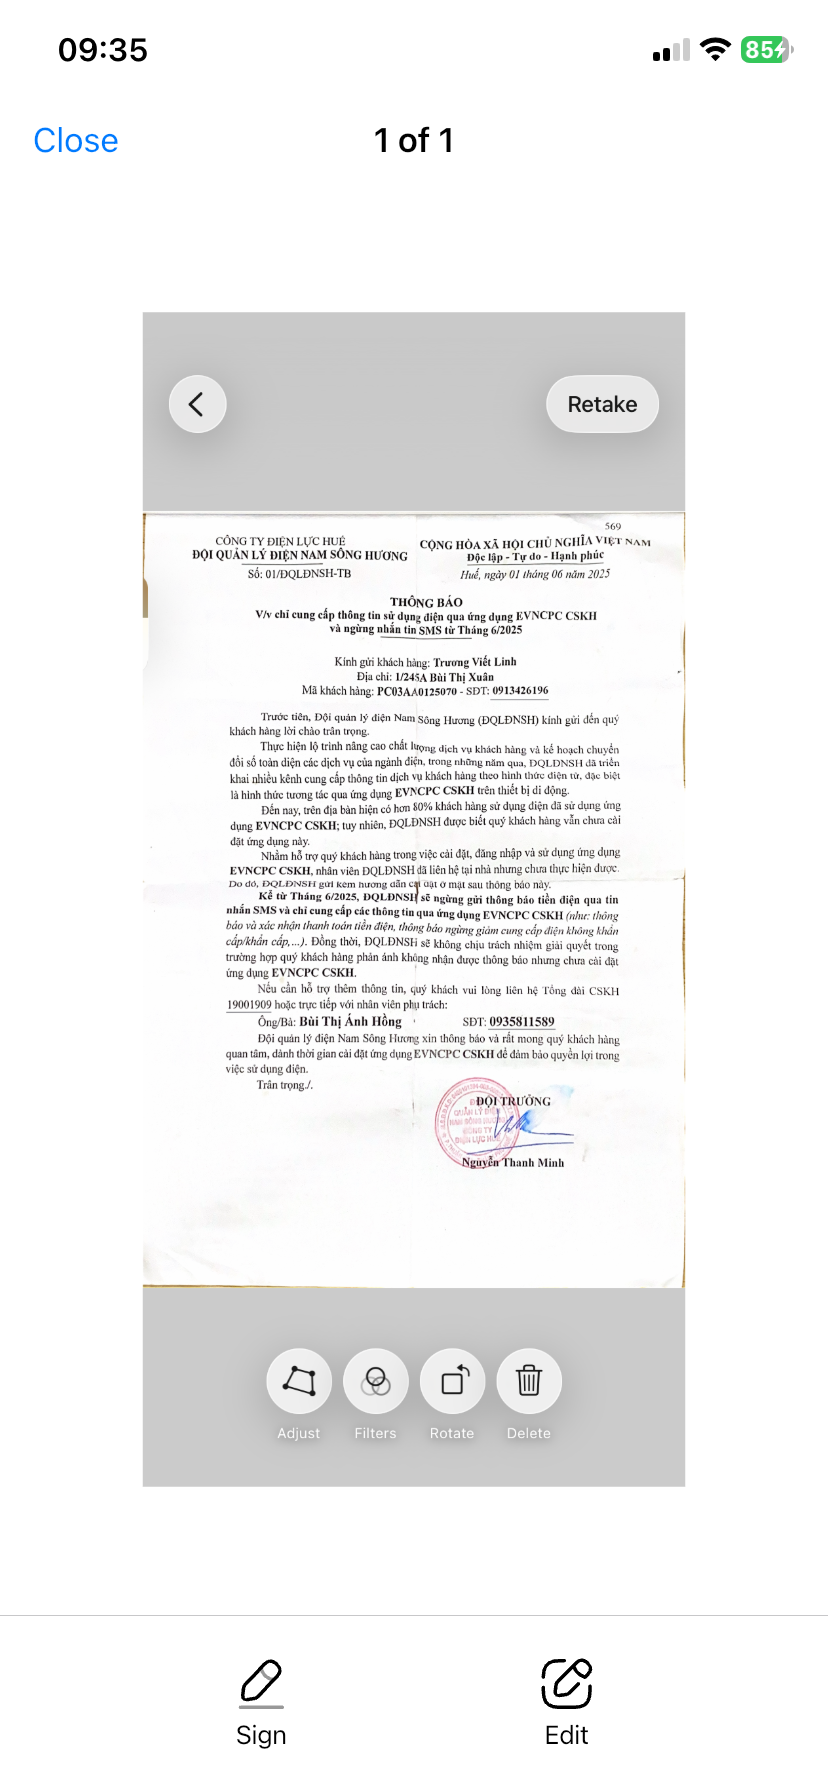
\includegraphics[height=9.5cm]{features/IMG_7588.PNG}
        \caption{Màn hình ``Choose signature'': tạo New signature hoặc chọn lại chữ ký đã lưu (Saved 1, Saved 2).}
        \label{fig:pdf_choose_sig}
    \end{minipage}
    \hfill
    \begin{minipage}{0.45\textwidth}
        \centering
        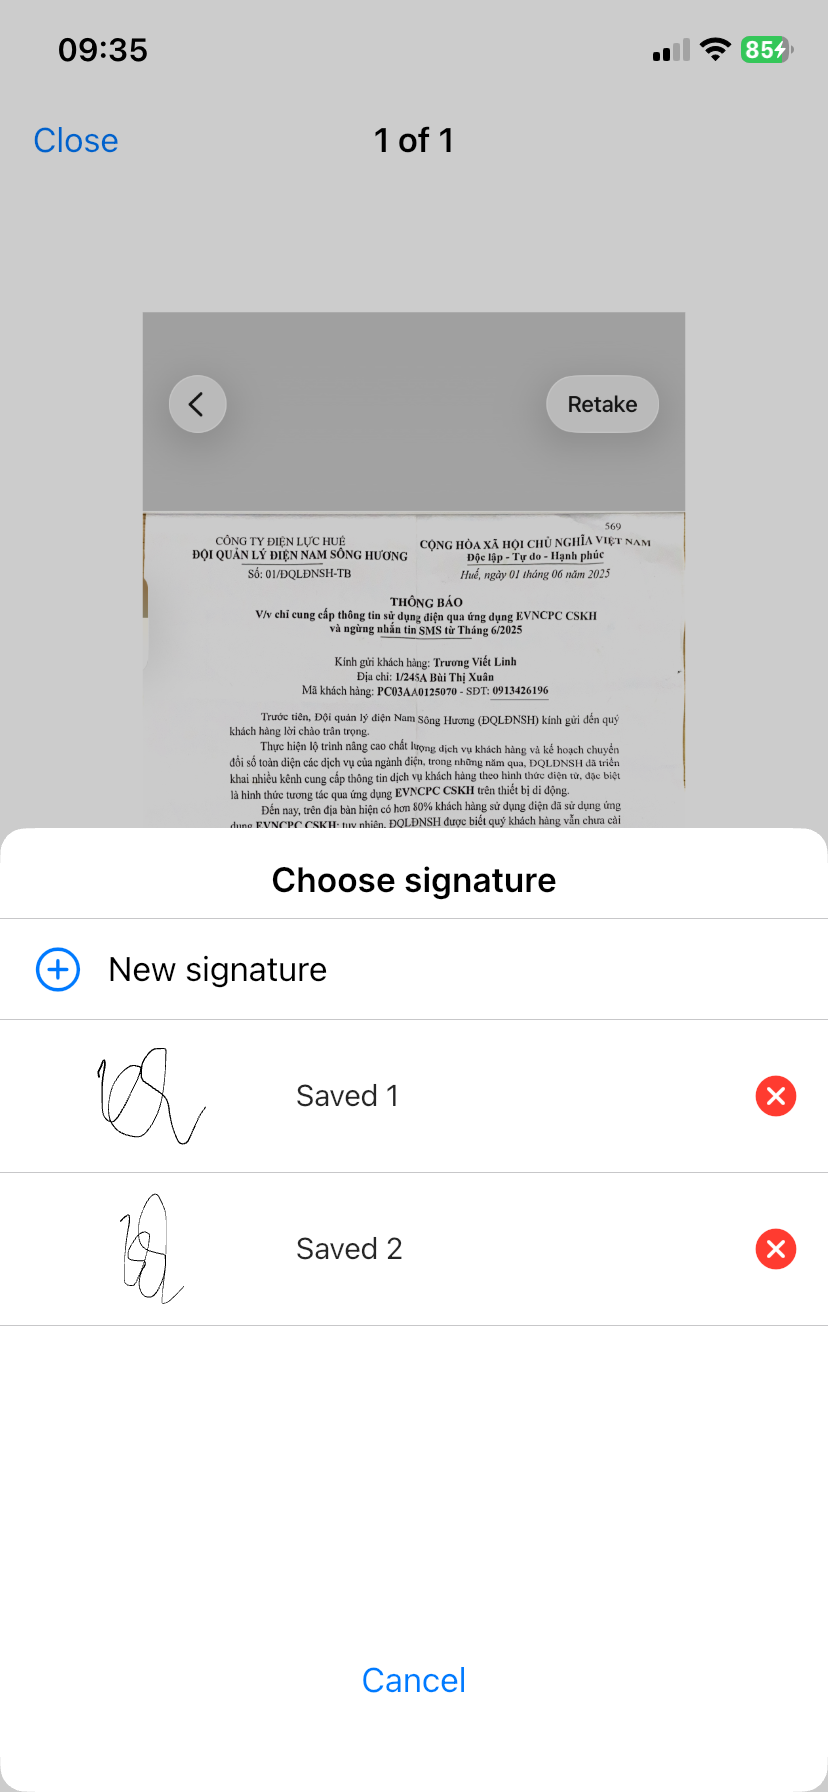
\includegraphics[height=9.5cm]{features/IMG_7589.PNG}
        \caption{Canvas vẽ chữ ký tay (Draw Signature) chế độ ngang với bộ chọn màu mực (Đỏ/Xanh/Đen) and slider độ dày nét.}
        \label{fig:pdf_draw_sig}
    \end{minipage}
\end{figure}

\begin{figure}[htbp]
    \centering
    \begin{minipage}{0.45\textwidth}
        \centering
        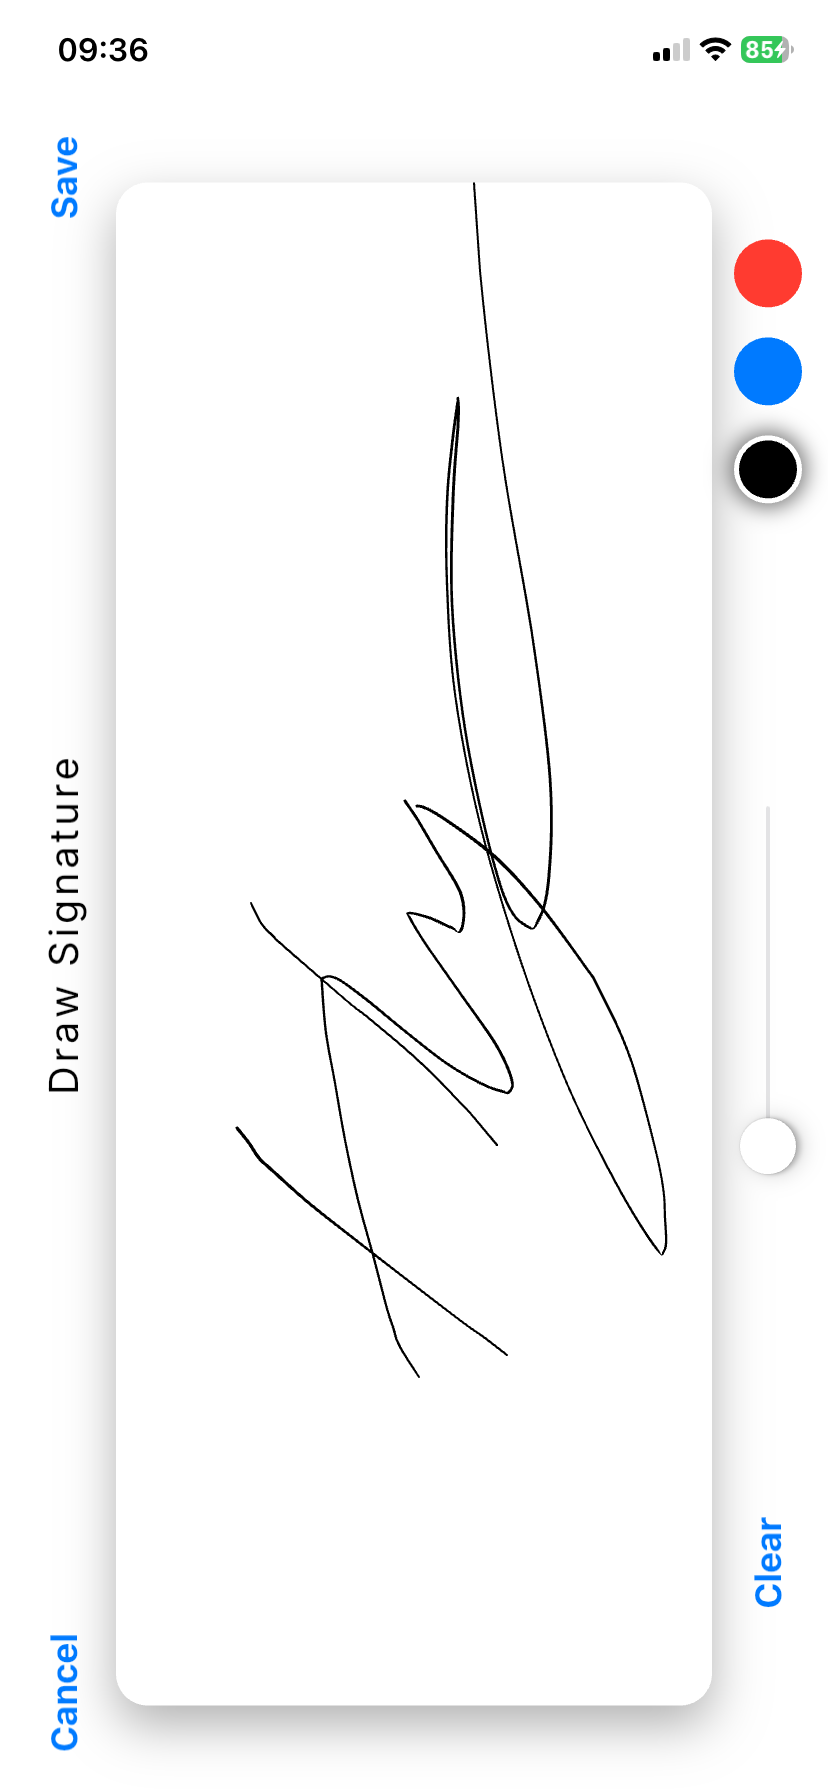
\includegraphics[height=9.5cm]{features/IMG_7590.PNG}
        \caption{Đặt chữ ký tay số lên trang PDF: tương tác kéo thả, xoay tự do, xóa bằng nút đỏ trực quan.}
        \label{fig:pdf_sign_on_page}
    \end{minipage}
    \hfill
    \begin{minipage}{0.45\textwidth}
        \centering
        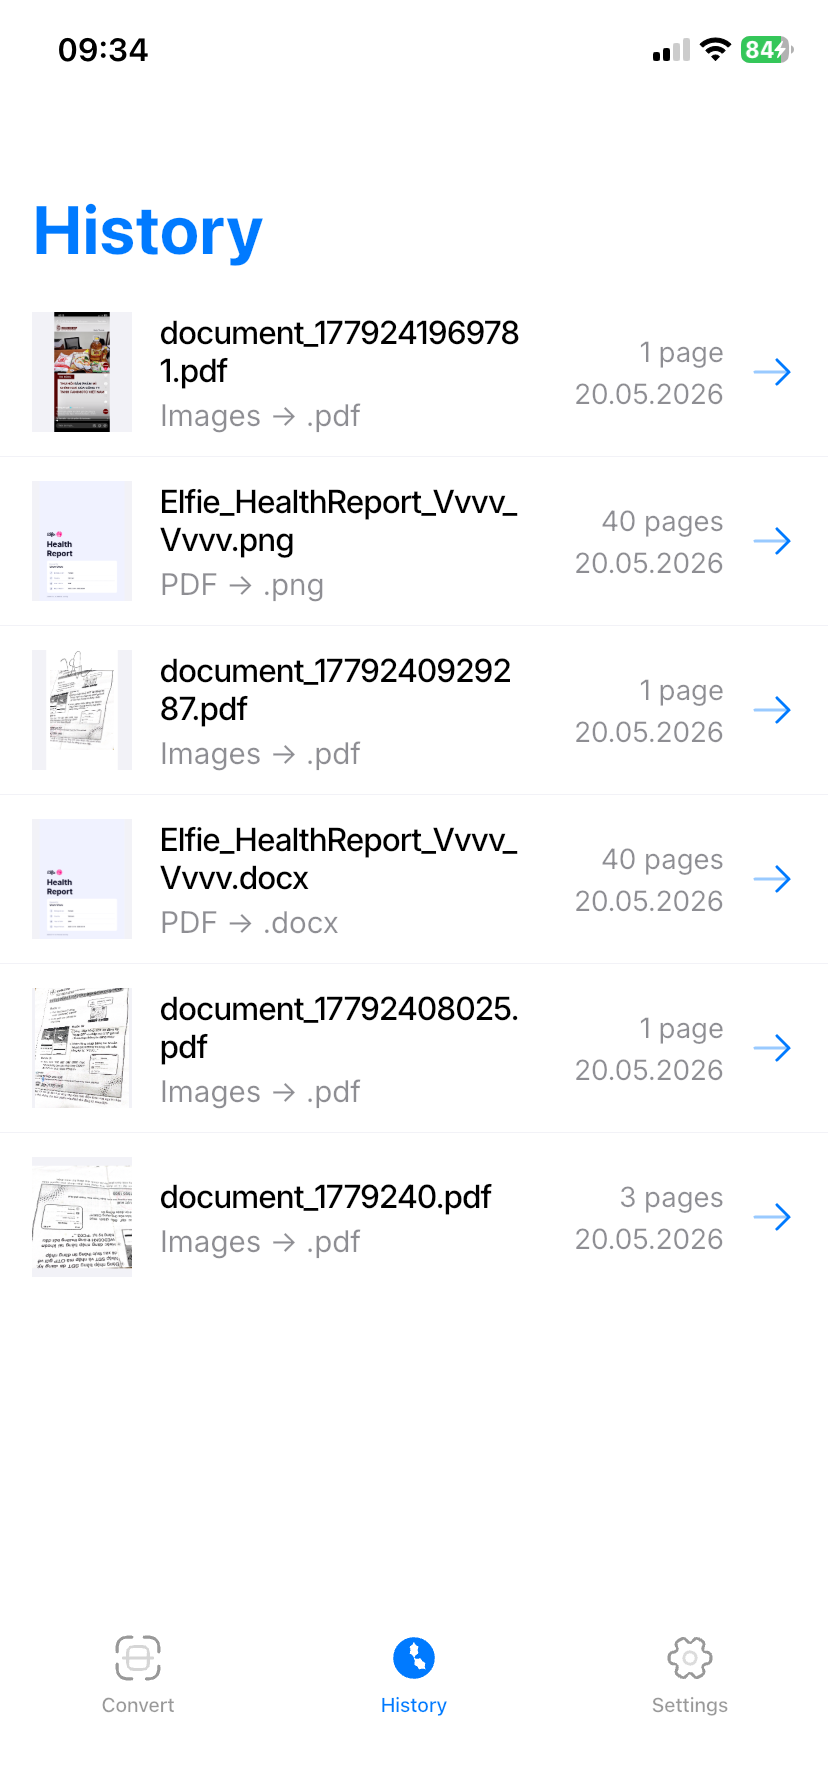
\includegraphics[height=9.5cm]{features/IMG_7577.PNG}
        \caption{Màn hình History: lịch sử toàn bộ tài liệu đã chuyển đổi kèm thumbnail, tên tệp, định dạng nguồn$\rightarrow$đích, số trang và ngày giờ (Isar DB).}
        \label{fig:pdf_history}
    \end{minipage}
\end{figure}

\newpage
\subsubsection*{3.6. Cài đặt ứng dụng và Đa ngôn ngữ}
\begin{figure}[htbp]
    \centering
    \begin{minipage}{0.45\textwidth}
        \centering
        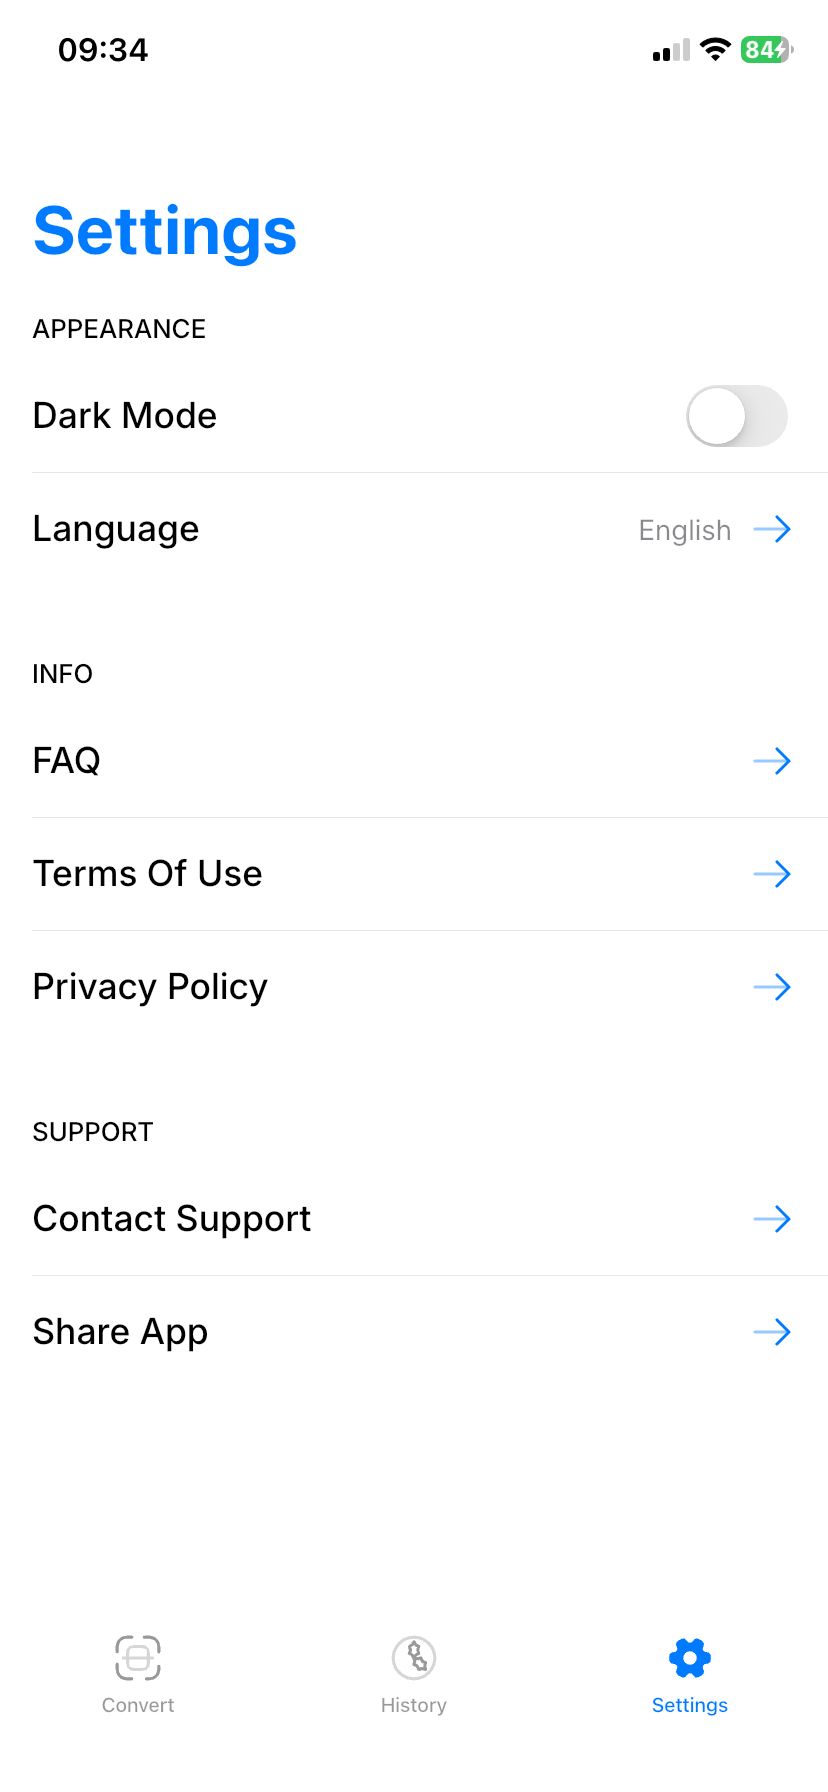
\includegraphics[height=9.5cm]{features/IMG_7578.PNG}
        \caption{Màn hình Settings: tùy chỉnh Dark Mode, Language, FAQ, Terms Of Use, Privacy Policy, Contact Support, Share App.}
        \label{fig:pdf_settings}
    \end{minipage}
    \hfill
    \begin{minipage}{0.45\textwidth}
        \centering
        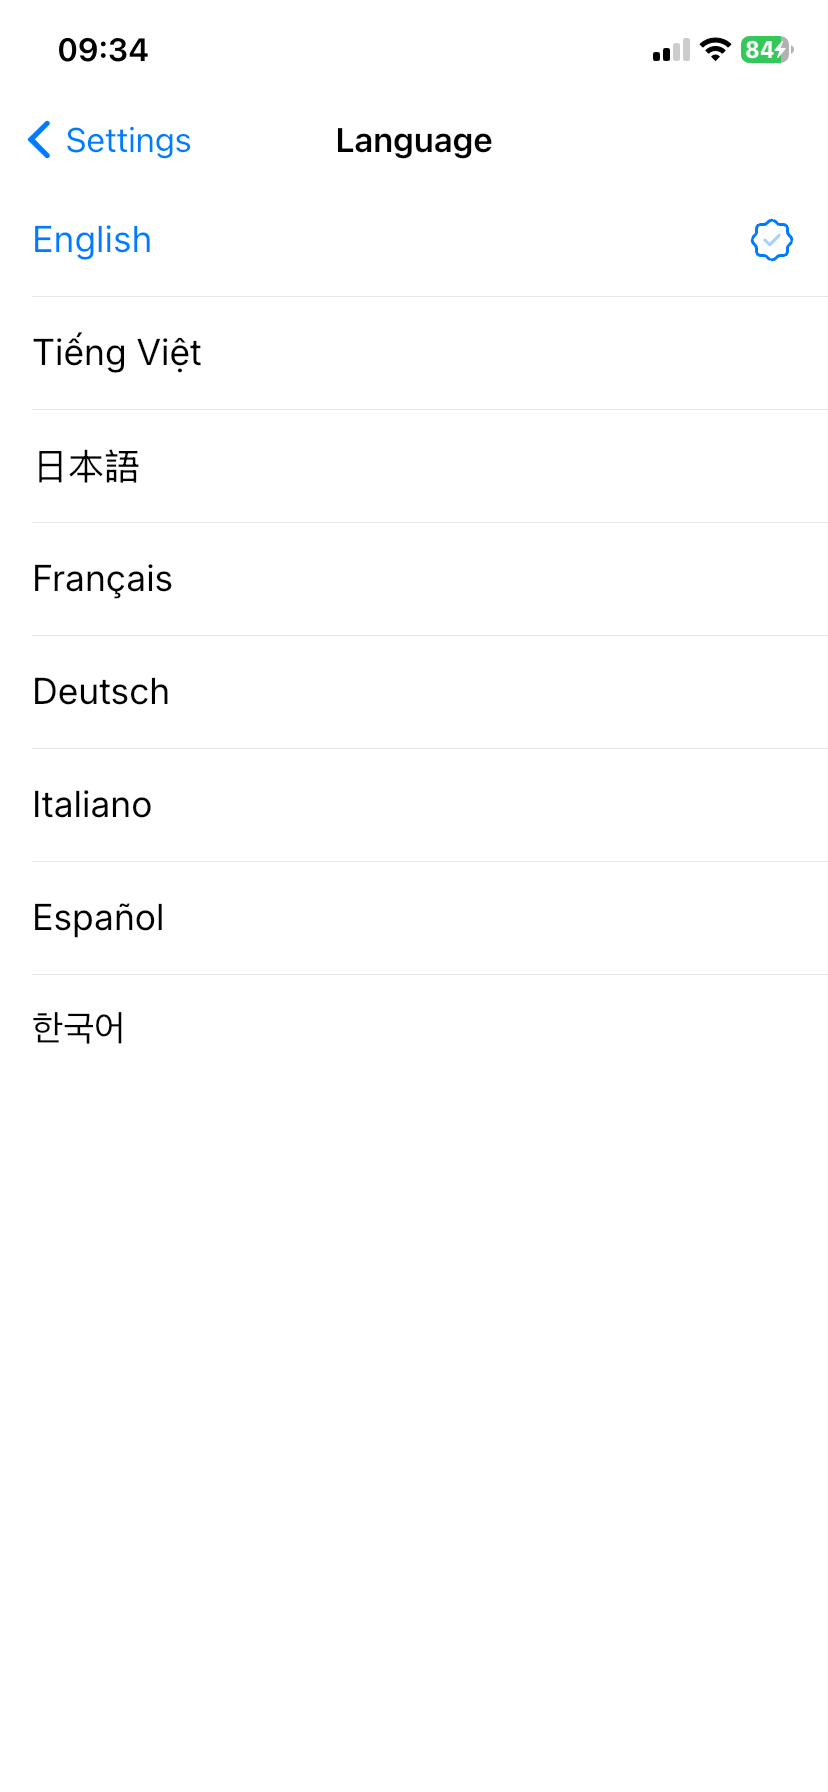
\includegraphics[height=9.5cm]{features/IMG_7579.PNG}
        \caption{Màn hình Language: hỗ trợ 8 ngôn ngữ giao diện (English, Tiếng Việt, Japanese, Français, Deutsch, Italiano, Español, Korean).}
        \label{fig:pdf_language}
    \end{minipage}
\end{figure}

\newpage
\subsection*{Phần 4: Dự án Ad-Free Blood Pressure App (Giai đoạn 4)}
Ứng dụng tự phát triển và phát hành thành công trên App Store:

\begin{figure}[htbp]
    \centering
    \begin{minipage}{0.45\textwidth}
        \centering
        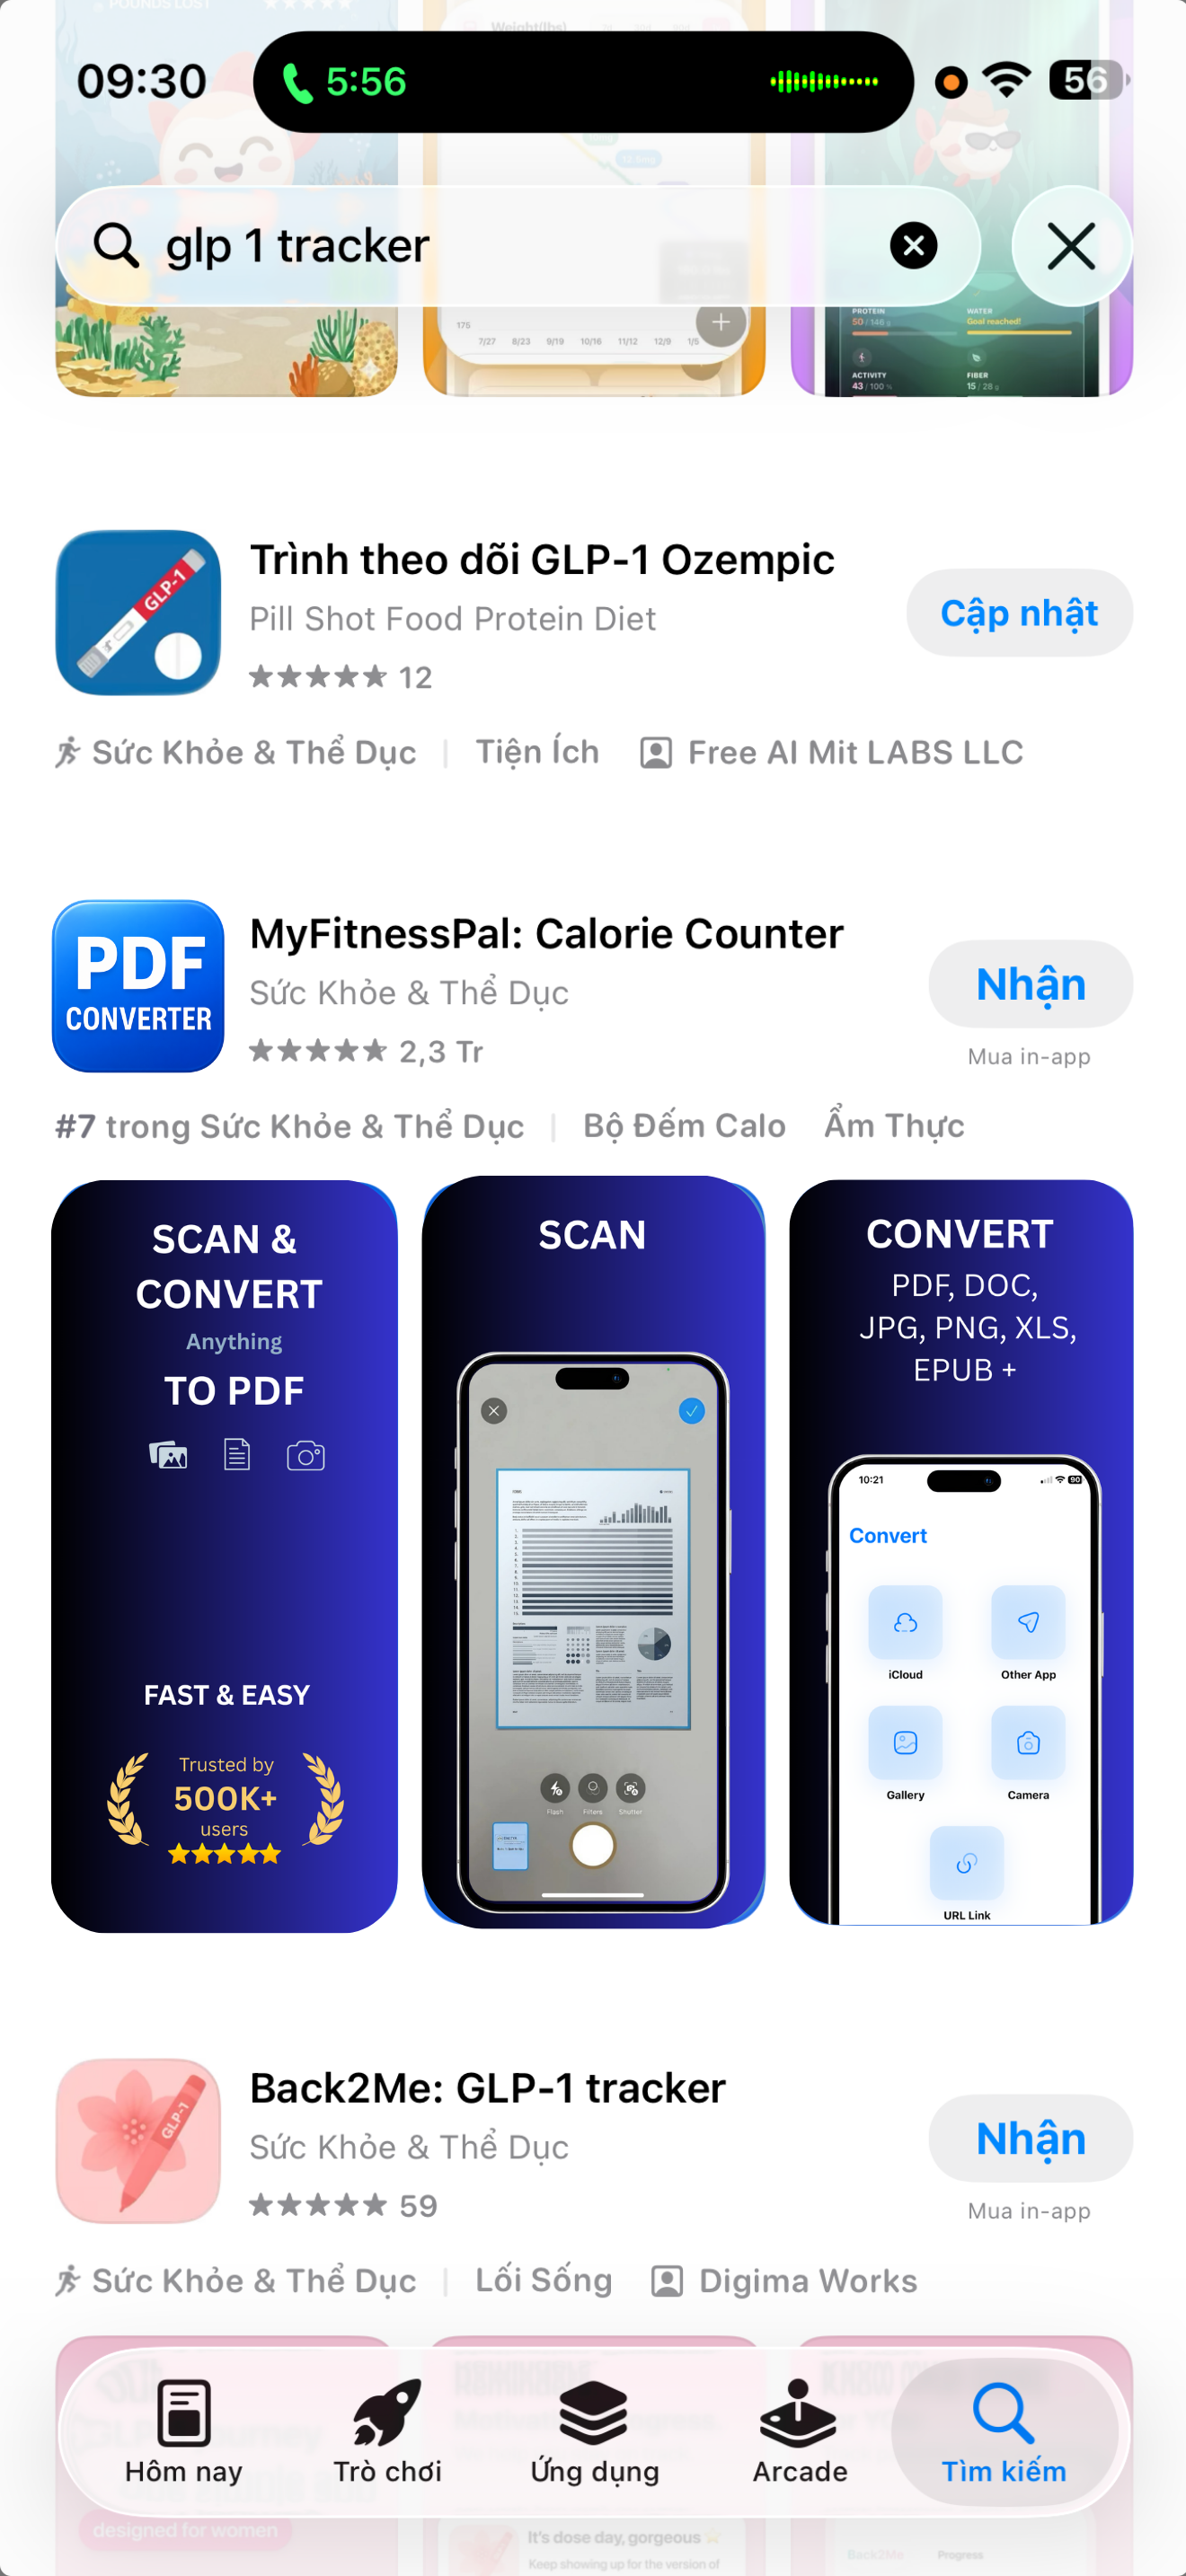
\includegraphics[width=\textwidth]{demo_app_store/1.png}\\
        \vspace{0.1cm}
        \scriptsize Giao diện App Store (Chế độ Sáng)
    \end{minipage}
    \hfill
    \begin{minipage}{0.45\textwidth}
        \centering
        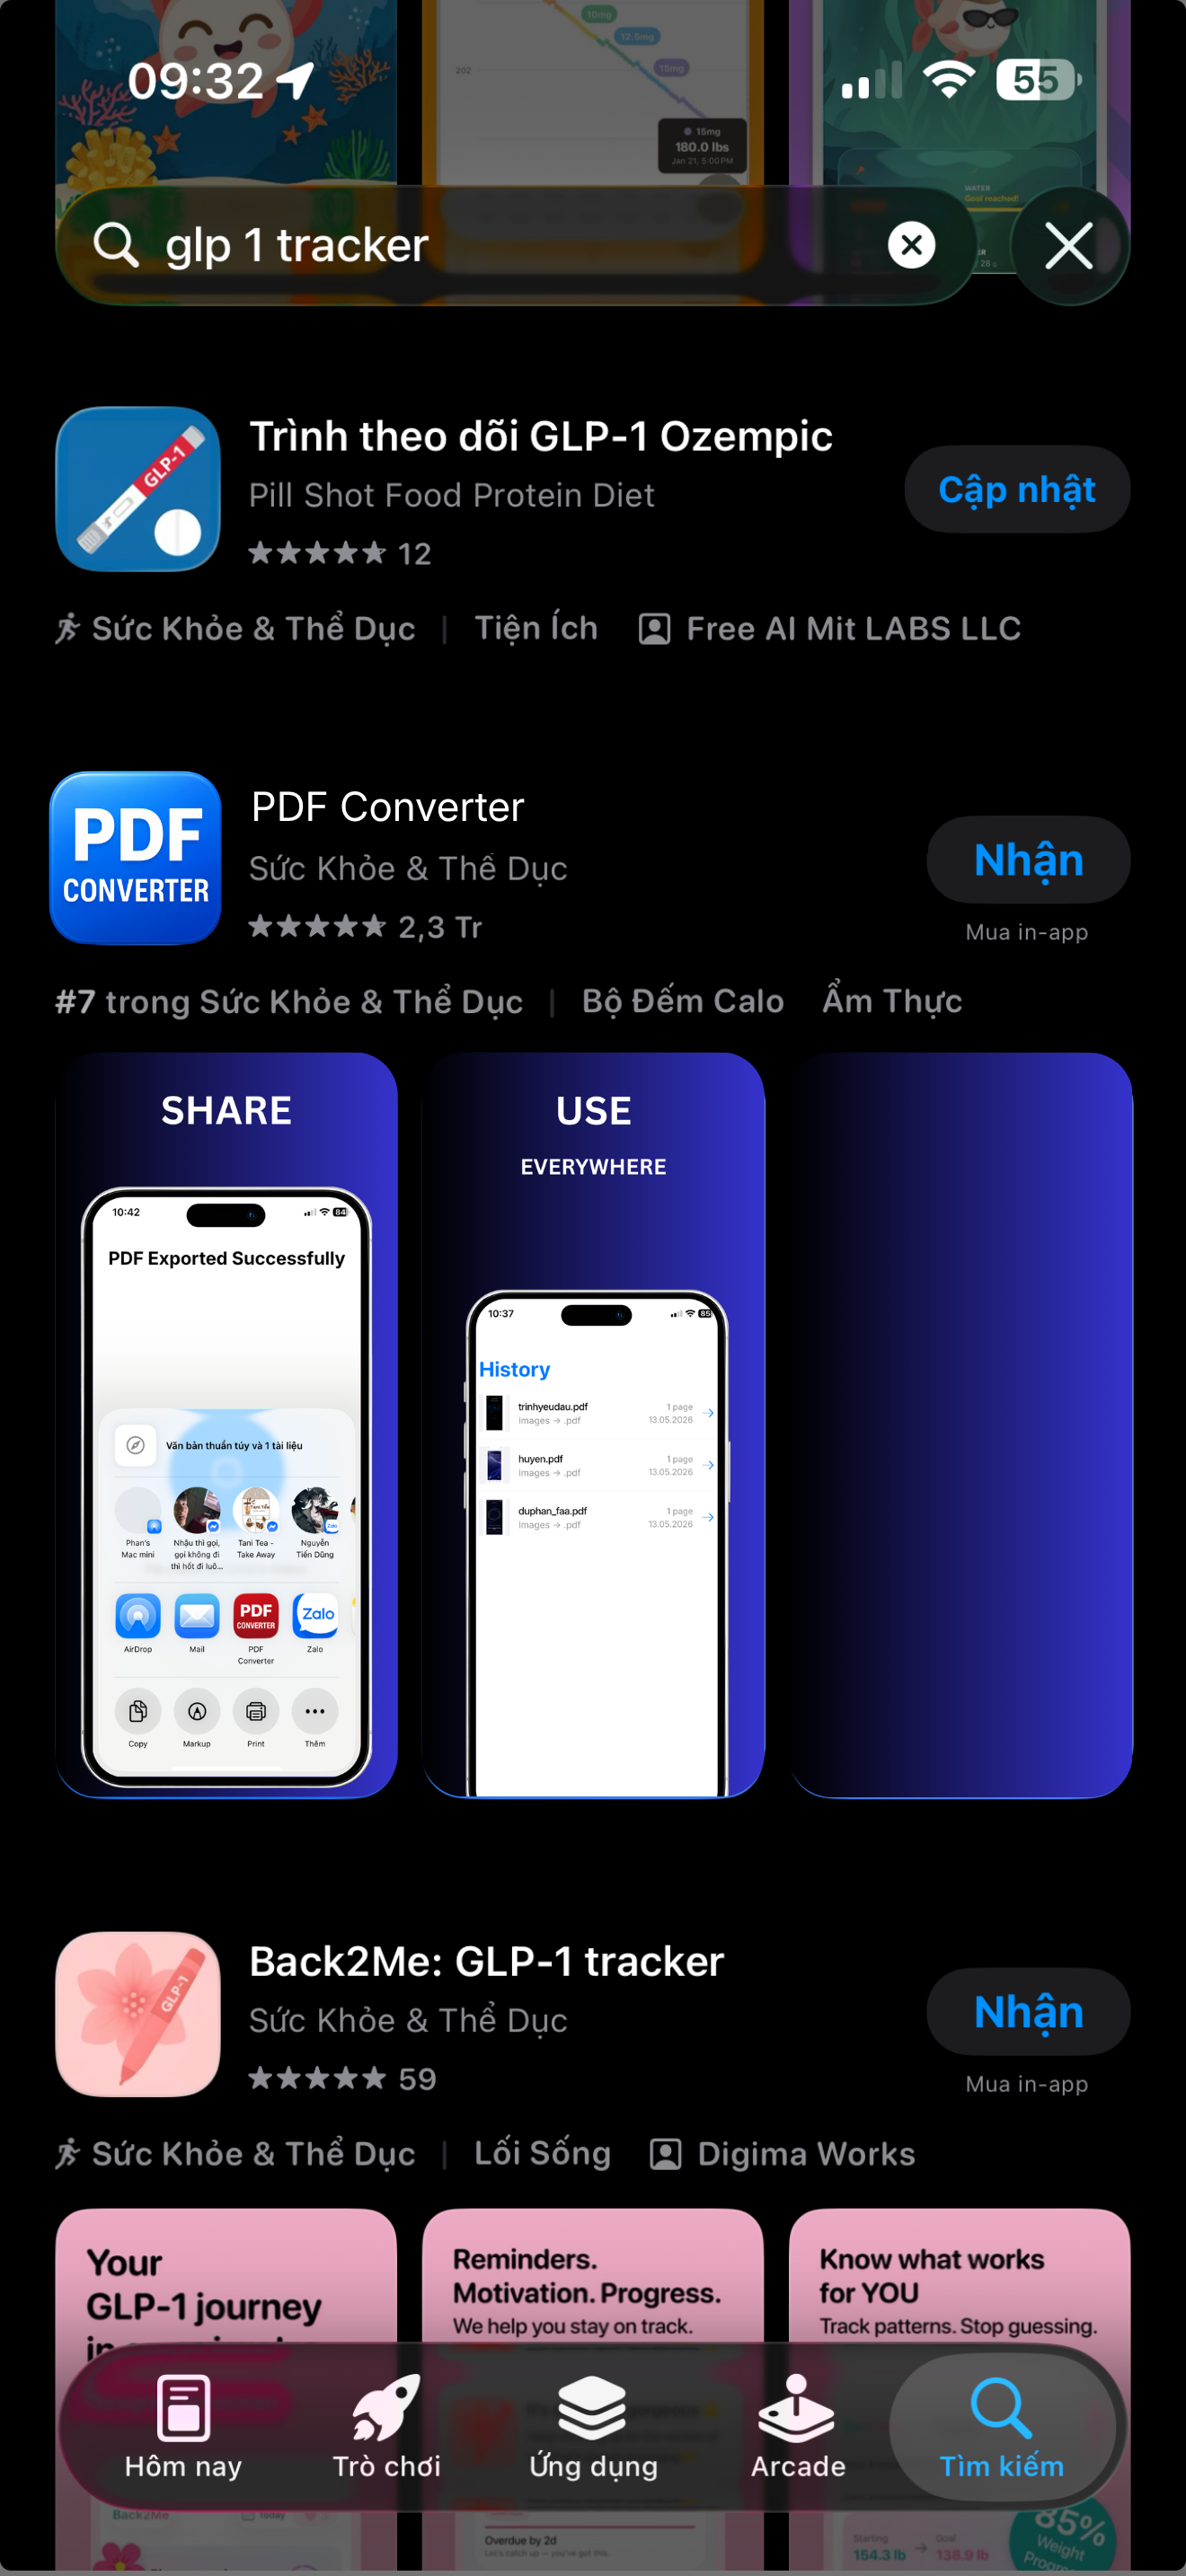
\includegraphics[width=\textwidth]{demo_app_store/2.png}\\
        \vspace{0.1cm}
        \scriptsize Giao diện App Store (Chế độ Tối)
    \end{minipage}
\end{figure}

\end{document}
